% Options for packages loaded elsewhere
\PassOptionsToPackage{unicode}{hyperref}
\PassOptionsToPackage{hyphens}{url}
%
\documentclass[
]{book}
\usepackage{amsmath,amssymb}
\usepackage{iftex}
\ifPDFTeX
  \usepackage[T1]{fontenc}
  \usepackage[utf8]{inputenc}
  \usepackage{textcomp} % provide euro and other symbols
\else % if luatex or xetex
  \usepackage{unicode-math} % this also loads fontspec
  \defaultfontfeatures{Scale=MatchLowercase}
  \defaultfontfeatures[\rmfamily]{Ligatures=TeX,Scale=1}
\fi
\usepackage{lmodern}
\ifPDFTeX\else
  % xetex/luatex font selection
\fi
% Use upquote if available, for straight quotes in verbatim environments
\IfFileExists{upquote.sty}{\usepackage{upquote}}{}
\IfFileExists{microtype.sty}{% use microtype if available
  \usepackage[]{microtype}
  \UseMicrotypeSet[protrusion]{basicmath} % disable protrusion for tt fonts
}{}
\makeatletter
\@ifundefined{KOMAClassName}{% if non-KOMA class
  \IfFileExists{parskip.sty}{%
    \usepackage{parskip}
  }{% else
    \setlength{\parindent}{0pt}
    \setlength{\parskip}{6pt plus 2pt minus 1pt}}
}{% if KOMA class
  \KOMAoptions{parskip=half}}
\makeatother
\usepackage{xcolor}
\usepackage{color}
\usepackage{fancyvrb}
\newcommand{\VerbBar}{|}
\newcommand{\VERB}{\Verb[commandchars=\\\{\}]}
\DefineVerbatimEnvironment{Highlighting}{Verbatim}{commandchars=\\\{\}}
% Add ',fontsize=\small' for more characters per line
\usepackage{framed}
\definecolor{shadecolor}{RGB}{248,248,248}
\newenvironment{Shaded}{\begin{snugshade}}{\end{snugshade}}
\newcommand{\AlertTok}[1]{\textcolor[rgb]{0.94,0.16,0.16}{#1}}
\newcommand{\AnnotationTok}[1]{\textcolor[rgb]{0.56,0.35,0.01}{\textbf{\textit{#1}}}}
\newcommand{\AttributeTok}[1]{\textcolor[rgb]{0.13,0.29,0.53}{#1}}
\newcommand{\BaseNTok}[1]{\textcolor[rgb]{0.00,0.00,0.81}{#1}}
\newcommand{\BuiltInTok}[1]{#1}
\newcommand{\CharTok}[1]{\textcolor[rgb]{0.31,0.60,0.02}{#1}}
\newcommand{\CommentTok}[1]{\textcolor[rgb]{0.56,0.35,0.01}{\textit{#1}}}
\newcommand{\CommentVarTok}[1]{\textcolor[rgb]{0.56,0.35,0.01}{\textbf{\textit{#1}}}}
\newcommand{\ConstantTok}[1]{\textcolor[rgb]{0.56,0.35,0.01}{#1}}
\newcommand{\ControlFlowTok}[1]{\textcolor[rgb]{0.13,0.29,0.53}{\textbf{#1}}}
\newcommand{\DataTypeTok}[1]{\textcolor[rgb]{0.13,0.29,0.53}{#1}}
\newcommand{\DecValTok}[1]{\textcolor[rgb]{0.00,0.00,0.81}{#1}}
\newcommand{\DocumentationTok}[1]{\textcolor[rgb]{0.56,0.35,0.01}{\textbf{\textit{#1}}}}
\newcommand{\ErrorTok}[1]{\textcolor[rgb]{0.64,0.00,0.00}{\textbf{#1}}}
\newcommand{\ExtensionTok}[1]{#1}
\newcommand{\FloatTok}[1]{\textcolor[rgb]{0.00,0.00,0.81}{#1}}
\newcommand{\FunctionTok}[1]{\textcolor[rgb]{0.13,0.29,0.53}{\textbf{#1}}}
\newcommand{\ImportTok}[1]{#1}
\newcommand{\InformationTok}[1]{\textcolor[rgb]{0.56,0.35,0.01}{\textbf{\textit{#1}}}}
\newcommand{\KeywordTok}[1]{\textcolor[rgb]{0.13,0.29,0.53}{\textbf{#1}}}
\newcommand{\NormalTok}[1]{#1}
\newcommand{\OperatorTok}[1]{\textcolor[rgb]{0.81,0.36,0.00}{\textbf{#1}}}
\newcommand{\OtherTok}[1]{\textcolor[rgb]{0.56,0.35,0.01}{#1}}
\newcommand{\PreprocessorTok}[1]{\textcolor[rgb]{0.56,0.35,0.01}{\textit{#1}}}
\newcommand{\RegionMarkerTok}[1]{#1}
\newcommand{\SpecialCharTok}[1]{\textcolor[rgb]{0.81,0.36,0.00}{\textbf{#1}}}
\newcommand{\SpecialStringTok}[1]{\textcolor[rgb]{0.31,0.60,0.02}{#1}}
\newcommand{\StringTok}[1]{\textcolor[rgb]{0.31,0.60,0.02}{#1}}
\newcommand{\VariableTok}[1]{\textcolor[rgb]{0.00,0.00,0.00}{#1}}
\newcommand{\VerbatimStringTok}[1]{\textcolor[rgb]{0.31,0.60,0.02}{#1}}
\newcommand{\WarningTok}[1]{\textcolor[rgb]{0.56,0.35,0.01}{\textbf{\textit{#1}}}}
\usepackage{longtable,booktabs,array}
\usepackage{calc} % for calculating minipage widths
% Correct order of tables after \paragraph or \subparagraph
\usepackage{etoolbox}
\makeatletter
\patchcmd\longtable{\par}{\if@noskipsec\mbox{}\fi\par}{}{}
\makeatother
% Allow footnotes in longtable head/foot
\IfFileExists{footnotehyper.sty}{\usepackage{footnotehyper}}{\usepackage{footnote}}
\makesavenoteenv{longtable}
\usepackage{graphicx}
\makeatletter
\def\maxwidth{\ifdim\Gin@nat@width>\linewidth\linewidth\else\Gin@nat@width\fi}
\def\maxheight{\ifdim\Gin@nat@height>\textheight\textheight\else\Gin@nat@height\fi}
\makeatother
% Scale images if necessary, so that they will not overflow the page
% margins by default, and it is still possible to overwrite the defaults
% using explicit options in \includegraphics[width, height, ...]{}
\setkeys{Gin}{width=\maxwidth,height=\maxheight,keepaspectratio}
% Set default figure placement to htbp
\makeatletter
\def\fps@figure{htbp}
\makeatother
\setlength{\emergencystretch}{3em} % prevent overfull lines
\providecommand{\tightlist}{%
  \setlength{\itemsep}{0pt}\setlength{\parskip}{0pt}}
\setcounter{secnumdepth}{5}
\usepackage{booktabs}
\usepackage[scale = 0.9]{geometry}
\ifLuaTeX
  \usepackage{selnolig}  % disable illegal ligatures
\fi
\usepackage[]{natbib}
\bibliographystyle{plainnat}
\IfFileExists{bookmark.sty}{\usepackage{bookmark}}{\usepackage{hyperref}}
\IfFileExists{xurl.sty}{\usepackage{xurl}}{} % add URL line breaks if available
\urlstyle{same}
\hypersetup{
  pdftitle={Financial Econometrics - Tutorials},
  pdfauthor={Alessandro Ciancetta},
  hidelinks,
  pdfcreator={LaTeX via pandoc}}

\title{Financial Econometrics - Tutorials}
\author{Alessandro Ciancetta}
\date{Last update: February 26, 2024}

\begin{document}
\maketitle

{
\setcounter{tocdepth}{1}
\tableofcontents
}
\hypertarget{about}{%
\chapter*{About}\label{about}}
\addcontentsline{toc}{chapter}{About}

TA materials for the Financial Econometrics course held by Prof.~Christian Brownlees at the Barcelona School of Economics.

\begin{center}\includegraphics[width=1\linewidth]{pic_finmetrics} \end{center}

\hypertarget{session01}{%
\chapter{Introduction to time series}\label{session01}}

\hypertarget{stochastic-processes-and-dependence}{%
\section{Stochastic processes and dependence}\label{stochastic-processes-and-dependence}}

Stochastic processes are a tool for modeling dependence in consecutive random variables \(\{\dots, Y_{-2}, Y_{-1}, Y_{0}, Y_{1}, Y_{2} \dots\}\). However, in practice, when we observe an empirical time series we are considering \emph{one, truncated} realization of the stochastic process, \(\{y_1, y_2, \dots, y_T\}\). As it is easy to imagine, this can cause some issues in studying the properties of an empirical time series. First, because we can only study the \emph{finite} dimensional distribution of the process. Second, because our task is to learn something about the process by knowing only one realization of it.

To overcome this limitations we need assumptions. In particular, two common assumptions in time series analysis are, loosely speaking:

\begin{itemize}
\item
  stationarity: the observed values in the sequence come from the same distribution, so that it is possible to learn from the past observations and to generalize the results to the entire, infinite stochastic process
\item
  ergodicity: values observed far away in time can be considered as independent, and hence if we have enough observations the empirical time series is representative of the entire distribution of the stochastic process
\end{itemize}

Under these (or similar) assumptions, we can use the observations from a single empirical time series to learn the parameters of our models.

\hypertarget{stationarity}{%
\subsection*{Stationarity}\label{stationarity}}
\addcontentsline{toc}{subsection}{Stationarity}

Consider the example in the plot below. If we had only observations laying between two changepoints we would not be able to retrieve the dynamics of the underlying process. For instance, if we observed a series ending before the first changepoint, we would have no information about the future realizations of the process. Indeed, future observations would come from different distributions that we could not learn from available information.

\begin{Shaded}
\begin{Highlighting}[]
\DocumentationTok{\#\# Example 1: non{-}stationary process}
\CommentTok{\# simulation}
\NormalTok{t\_max }\OtherTok{\textless{}{-}} \DecValTok{500}
\NormalTok{y }\OtherTok{\textless{}{-}} \FunctionTok{rep}\NormalTok{(}\ConstantTok{NA}\NormalTok{, t\_max)}
\ControlFlowTok{for}\NormalTok{ (t }\ControlFlowTok{in} \DecValTok{1}\SpecialCharTok{:}\NormalTok{t\_max) \{}
  \ControlFlowTok{if}\NormalTok{ (t}\SpecialCharTok{\textless{}=}\DecValTok{100}\NormalTok{) \{}
\NormalTok{    y[t] }\OtherTok{\textless{}{-}} \FunctionTok{rnorm}\NormalTok{(}\DecValTok{1}\NormalTok{, }\AttributeTok{mean =} \DecValTok{0}\NormalTok{, }\AttributeTok{sd =} \FloatTok{0.1}\NormalTok{)}
\NormalTok{  \}}
  \ControlFlowTok{if}\NormalTok{ (t}\SpecialCharTok{\textgreater{}}\DecValTok{100} \SpecialCharTok{\&}\NormalTok{ t}\SpecialCharTok{\textless{}=}\DecValTok{250}\NormalTok{) \{}
\NormalTok{    y[t] }\OtherTok{\textless{}{-}} \FunctionTok{rnorm}\NormalTok{(}\DecValTok{1}\NormalTok{, }\AttributeTok{mean =} \FloatTok{0.5}\NormalTok{, }\AttributeTok{sd =} \FloatTok{0.1}\NormalTok{)}
\NormalTok{  \}}
  \ControlFlowTok{if}\NormalTok{ (t}\SpecialCharTok{\textgreater{}}\DecValTok{250} \SpecialCharTok{\&}\NormalTok{ t}\SpecialCharTok{\textless{}=}\DecValTok{400}\NormalTok{) \{}
\NormalTok{    y[t] }\OtherTok{\textless{}{-}} \FunctionTok{rnorm}\NormalTok{(}\DecValTok{1}\NormalTok{, }\AttributeTok{mean =} \DecValTok{0}\NormalTok{, }\AttributeTok{sd =} \FloatTok{0.2}\NormalTok{)}
\NormalTok{  \}}
  \ControlFlowTok{if}\NormalTok{ (t}\SpecialCharTok{\textgreater{}}\DecValTok{400} \SpecialCharTok{\&}\NormalTok{ t}\SpecialCharTok{\textless{}=}\NormalTok{t\_max) \{}
\NormalTok{    y[t] }\OtherTok{\textless{}{-}} \FloatTok{0.01}\SpecialCharTok{*}\NormalTok{(t}\DecValTok{{-}400}\NormalTok{) }\SpecialCharTok{+} \FunctionTok{rnorm}\NormalTok{(}\DecValTok{1}\NormalTok{, }\AttributeTok{mean =} \SpecialCharTok{{-}}\FloatTok{0.2}\NormalTok{, }\AttributeTok{sd =} \FloatTok{0.02}\NormalTok{)}
\NormalTok{  \}}
\NormalTok{\}}
\CommentTok{\# plot}
\FunctionTok{plot.ts}\NormalTok{(y, }\AttributeTok{main =} \StringTok{"Non{-}stationary process"}\NormalTok{, }\AttributeTok{xaxt =} \StringTok{"n"}\NormalTok{)}
\FunctionTok{abline}\NormalTok{(}\AttributeTok{v =} \FunctionTok{c}\NormalTok{(}\DecValTok{100}\NormalTok{, }\DecValTok{250}\NormalTok{, }\DecValTok{400}\NormalTok{), }\AttributeTok{lty =} \DecValTok{2}\NormalTok{)}
\FunctionTok{axis}\NormalTok{(}\DecValTok{1}\NormalTok{, }\AttributeTok{at=}\FunctionTok{c}\NormalTok{(}\DecValTok{100}\NormalTok{, }\DecValTok{250}\NormalTok{, }\DecValTok{400}\NormalTok{),}
     \AttributeTok{labels =} \FunctionTok{c}\NormalTok{(}\StringTok{"Changepoint 1"}\NormalTok{, }\StringTok{"Changepoint 2"}\NormalTok{, }\StringTok{"Changepoint 3"}\NormalTok{))}
\end{Highlighting}
\end{Shaded}

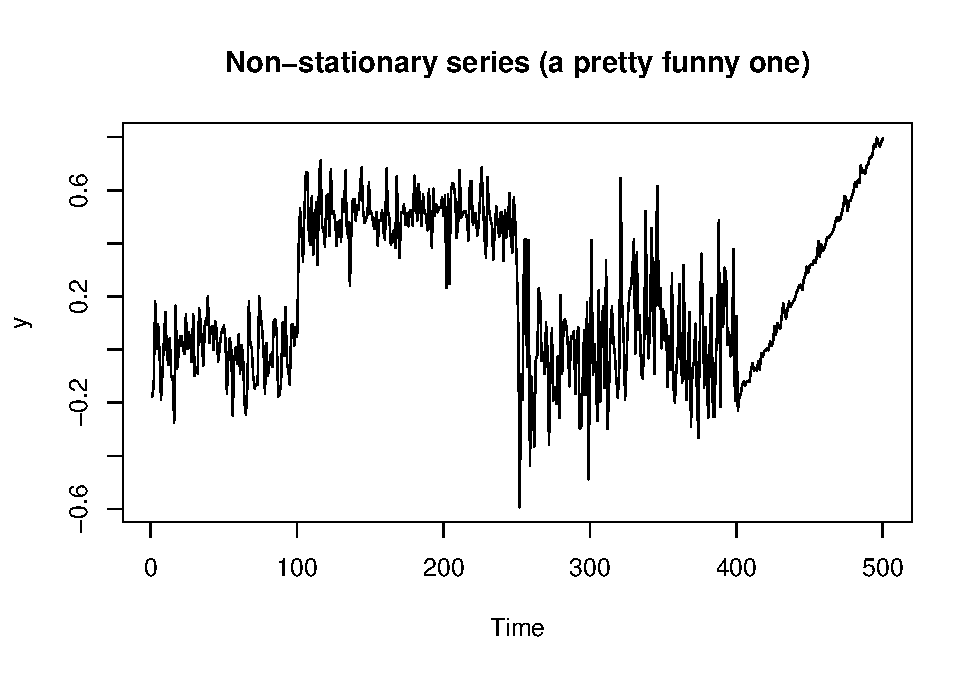
\includegraphics{_main_files/figure-latex/unnamed-chunk-3-1.pdf}

\hypertarget{ergodicity}{%
\subsection*{Ergodicity}\label{ergodicity}}
\addcontentsline{toc}{subsection}{Ergodicity}

Let \(\{z_t\}_{t = 1}^{T} \stackrel{iid}{\sim} \mathcal{N}(0, 1)\). Consider the two following data-generating processes:

\[
\begin{aligned}
y_t &= U_0 + 0.25z_t, \quad \text{with  } U_0 \sim \mathcal{N}(0, 100) \\[1ex]
x_t &= z_t + z_{t-1}
\end{aligned}
\]

We have:

\[
\begin{aligned}
\mathbb{E}[y_t] &= \mathbb{E}[x_t] = 0 \\[1em]
\text{cov}(y_t, y_{t-k}) &= 
\begin{cases}
100+0.25^2 & k = 0 \\
100 & k \neq 0
\end{cases} \\[1ex]
\text{cov}(x_t, x_{t-k}) &= 
\begin{cases}
2 & k = 0 \\
1 & k = 1 \\
0 & k \geq 2
\end{cases}
\end{aligned}
\]

We now simulate the two data generating processes in \texttt{R}. We want to draw many sequences \(\{y_1, \dots, y_T\}^{(s)}, \{x_1, \dots, x_T\}^{(s)}\) for \(s = 1, \dots, S\) simulations to assess whether observing a single time series is enough to estimate the mean of the processes.

\begin{Shaded}
\begin{Highlighting}[]
\DocumentationTok{\#\# Example 2: weak dependence}

\DocumentationTok{\#\# Simulate process y\_t}
\CommentTok{\# initialize TxS matrix to store result }
\CommentTok{\# (each column is a simulated time series \{y\_1, ..., y\_T\}\^{}(s) )}
\NormalTok{nsim }\OtherTok{\textless{}{-}} \DecValTok{3}
\NormalTok{y\_list }\OtherTok{\textless{}{-}} \FunctionTok{matrix}\NormalTok{(}\FunctionTok{rep}\NormalTok{(}\ConstantTok{NA}\NormalTok{, nsim}\SpecialCharTok{*}\NormalTok{t\_max), }\AttributeTok{nrow =}\NormalTok{ t\_max, }\AttributeTok{ncol =}\NormalTok{ nsim)}
\CommentTok{\# simulation}
\ControlFlowTok{for}\NormalTok{ (sim }\ControlFlowTok{in} \DecValTok{1}\SpecialCharTok{:}\NormalTok{nsim) \{}
  \FunctionTok{set.seed}\NormalTok{(sim}\SpecialCharTok{+}\DecValTok{123}\NormalTok{)}
\NormalTok{  U0 }\OtherTok{\textless{}{-}} \FunctionTok{rnorm}\NormalTok{(}\DecValTok{1}\NormalTok{, }\AttributeTok{sd =} \DecValTok{10}\NormalTok{)}
\NormalTok{  z  }\OtherTok{\textless{}{-}} \FunctionTok{rnorm}\NormalTok{(t\_max)}
\NormalTok{  y\_list[,sim] }\OtherTok{\textless{}{-}}\NormalTok{ U0 }\SpecialCharTok{+} \FloatTok{0.25}\SpecialCharTok{*}\NormalTok{z}
\NormalTok{\}}
\end{Highlighting}
\end{Shaded}

As the plot below shows, if we observe a single simulated time series we cannot correctly estimate the mean of the process \(\mathbb{E}[y_t]\) using the sample mean \(\bar{y}_T\). What the sample mean is actually estimating in this case is the \emph{conditional} expctation of \(y_t\) given the specific draw of the random intercept \(U_0\) in simulation \(s\): \(\mathbb{E}\left[y_t | U_0 = U_0^{(s)}\right] = U_0^{(s)}\). Notice that in this case, if we observe a new point for stochastic process \(y_t\) (green points in the plot) we are likely not able to forecast it correctly based on the previous observations of a single time series.

\begin{Shaded}
\begin{Highlighting}[]
\CommentTok{\# plot}
\FunctionTok{plot.ts}\NormalTok{(y\_list[,}\DecValTok{1}\NormalTok{], }\AttributeTok{ylim =} \FunctionTok{c}\NormalTok{(}\SpecialCharTok{{-}}\DecValTok{25}\NormalTok{, }\DecValTok{25}\NormalTok{), }\AttributeTok{main =} \StringTok{"Realizations of non{-}ergodic series"}\NormalTok{, }\AttributeTok{ylab =} \StringTok{"y"}\NormalTok{)}
\FunctionTok{lines}\NormalTok{(y\_list[,}\DecValTok{2}\NormalTok{], }\AttributeTok{col =} \StringTok{"steelblue"}\NormalTok{)}
\FunctionTok{lines}\NormalTok{(y\_list[,}\DecValTok{3}\NormalTok{], }\AttributeTok{col =} \StringTok{"tomato"}\NormalTok{)}
\ControlFlowTok{for}\NormalTok{ (point }\ControlFlowTok{in} \DecValTok{1}\SpecialCharTok{:}\DecValTok{100}\NormalTok{)\{}
  \FunctionTok{points}\NormalTok{(}\AttributeTok{x =} \DecValTok{501}\NormalTok{, }\FunctionTok{rnorm}\NormalTok{(}\DecValTok{1}\NormalTok{, }\DecValTok{0}\NormalTok{, }\DecValTok{10}\NormalTok{)}\SpecialCharTok{+}\FunctionTok{rnorm}\NormalTok{(}\DecValTok{1}\NormalTok{, }\DecValTok{0}\NormalTok{, }\DecValTok{1}\NormalTok{), }\AttributeTok{col =} \StringTok{"darkgreen"}\NormalTok{, }\AttributeTok{pch =} \DecValTok{4}\NormalTok{)}
\NormalTok{\}}
\FunctionTok{abline}\NormalTok{(}\AttributeTok{h =} \DecValTok{0}\NormalTok{, }\AttributeTok{col =} \StringTok{"black"}\NormalTok{, }\AttributeTok{lwd =} \DecValTok{2}\NormalTok{, }\AttributeTok{lty =} \DecValTok{2}\NormalTok{)}
\end{Highlighting}
\end{Shaded}

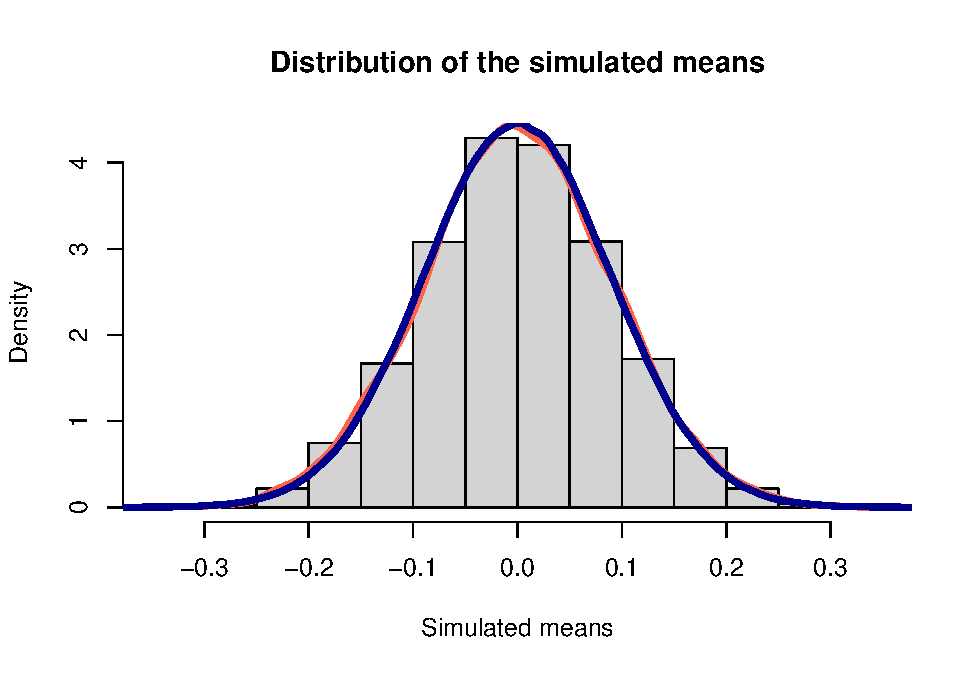
\includegraphics{_main_files/figure-latex/unnamed-chunk-5-1.pdf}

We now turn to process \(x_t\).

\begin{Shaded}
\begin{Highlighting}[]
\DocumentationTok{\#\# Simulate process x\_t}
\CommentTok{\# initialize object to store result}
\NormalTok{nsim }\OtherTok{\textless{}{-}} \DecValTok{10000}
\NormalTok{x\_list }\OtherTok{\textless{}{-}} \FunctionTok{matrix}\NormalTok{(}\FunctionTok{rep}\NormalTok{(}\ConstantTok{NA}\NormalTok{, nsim}\SpecialCharTok{*}\NormalTok{t\_max), }\AttributeTok{nrow =}\NormalTok{ t\_max, }\AttributeTok{ncol =}\NormalTok{ nsim)}
\CommentTok{\# simulation}
\ControlFlowTok{for}\NormalTok{ (sim }\ControlFlowTok{in} \DecValTok{1}\SpecialCharTok{:}\NormalTok{nsim) \{}
  \FunctionTok{set.seed}\NormalTok{(sim}\SpecialCharTok{+}\DecValTok{123}\NormalTok{)}
\NormalTok{  z  }\OtherTok{\textless{}{-}} \FunctionTok{rnorm}\NormalTok{(t\_max}\SpecialCharTok{+}\DecValTok{1}\NormalTok{)}
\NormalTok{  x\_list[,sim] }\OtherTok{\textless{}{-}}\NormalTok{ z[}\DecValTok{2}\SpecialCharTok{:}\NormalTok{(t\_max}\SpecialCharTok{+}\DecValTok{1}\NormalTok{)] }\SpecialCharTok{+}\NormalTok{ z[}\DecValTok{1}\SpecialCharTok{:}\NormalTok{t\_max]}
\NormalTok{\}}
\end{Highlighting}
\end{Shaded}

All the simulated time series have mean zero in this case. As a consequence, we can use the sample mean \(\bar{x}_T\) obtained from a single time series to estimate the (unconditional) mean of the process \(\mathbb{E}[x_t]\).

\begin{Shaded}
\begin{Highlighting}[]
\CommentTok{\# plot}
\FunctionTok{plot.ts}\NormalTok{(x\_list[,}\DecValTok{1}\NormalTok{], }\AttributeTok{ylim =} \FunctionTok{c}\NormalTok{(}\FunctionTok{min}\NormalTok{(x\_list), }\FunctionTok{max}\NormalTok{(x\_list)), }
        \AttributeTok{main =} \StringTok{"Realizations of ergodic series"}\NormalTok{, }\AttributeTok{ylab =} \StringTok{"x"}\NormalTok{)}
\FunctionTok{lines}\NormalTok{(x\_list[,}\DecValTok{2}\NormalTok{], }\AttributeTok{col =} \StringTok{"steelblue"}\NormalTok{)}
\FunctionTok{lines}\NormalTok{(x\_list[,}\DecValTok{3}\NormalTok{], }\AttributeTok{col =} \StringTok{"tomato"}\NormalTok{)}
\FunctionTok{abline}\NormalTok{(}\AttributeTok{h =} \DecValTok{0}\NormalTok{, }\AttributeTok{col =} \StringTok{"black"}\NormalTok{, }\AttributeTok{lwd =} \DecValTok{2}\NormalTok{, }\AttributeTok{lty =} \DecValTok{2}\NormalTok{)}
\end{Highlighting}
\end{Shaded}

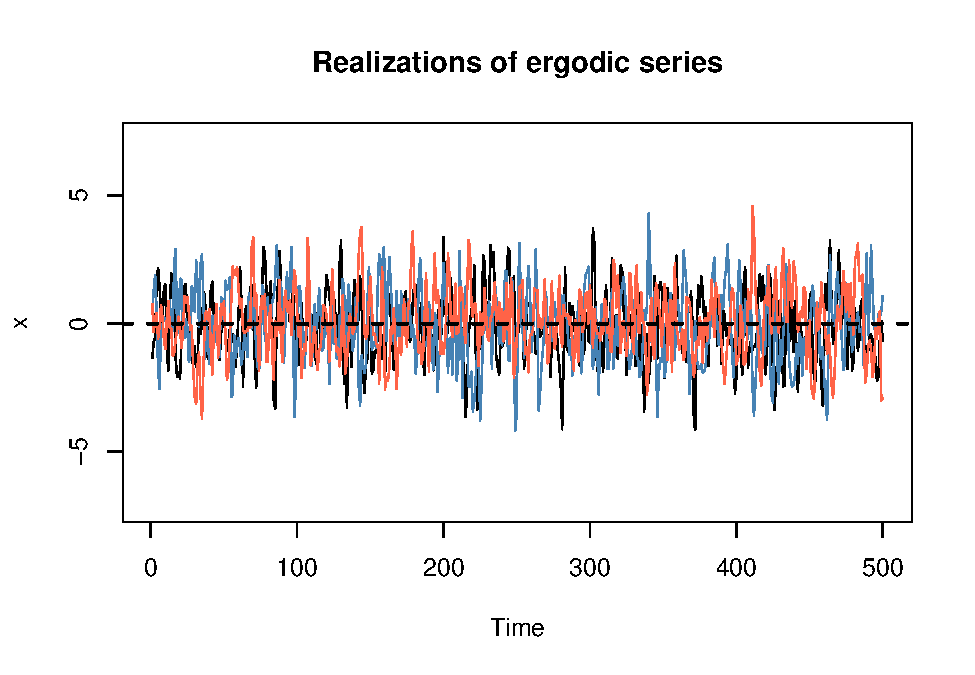
\includegraphics{_main_files/figure-latex/unnamed-chunk-7-1.pdf}

\hypertarget{asymptotic-results}{%
\section{Asymptotic results}\label{asymptotic-results}}

The problem with the series \(\{y_t\}\) in the previous example is that the autocovariance function does not decay as the lag order increases. Loosely speaking, the series gets stuck in the trajectory given by the initial draw of \(U_0\) and does not revert to the true mean of the stochastic process. The main consequence is that we cannot learn the mean of the process by taking the average of the observations in a single realized time series.

It is true in general that some conditions on the rate of decay of the autocovariance are required to recover the mean of the process. For example, the Law of Large Numbers (LLN) guarantees that the sample mean converges in probability to the true mean under the assumption that the autocovariances are absolutely summable:

\[
\sum_{k=0}^\infty |\gamma_k| < \infty
\]

Notice that in the case of \(\{y_t\}\) above instead \(\sum_{k=0}^\infty |\gamma_k| = \infty\). On the contrary, \(\{x_t\}\) satisfies both the conditions of the LLN and of the Central Limit Theorem (CLT). The condition for the latter is that \(\{\phi_k\}_{k=0}^\infty\) is absolutely summable in \(x_t = \mu_x + \sum_{k=0}^\infty\phi_k z_{t-k} = z_t + z_{t-1}\), which is trivially verified. Therefore, since \(\mu_x = 0\),

\[
\sqrt{T} \ \bar{x}_T  \ \xrightarrow{d} \ \mathcal{N}(0, \sigma^2_{LR}),
\]

with \(\sigma^2_{LR} = \sum_{k=-\infty}^\infty \gamma_k = \text{Var}(x_t) + 2\sum_{k=1}^\infty \gamma_k\).

\begin{Shaded}
\begin{Highlighting}[]
\DocumentationTok{\#\# Example 3: central limit theorem}
\NormalTok{x\_empirical }\OtherTok{\textless{}{-}}\NormalTok{ x\_list[,}\DecValTok{9}\NormalTok{]}
\NormalTok{x\_means }\OtherTok{\textless{}{-}} \FunctionTok{colMeans}\NormalTok{(x\_list)}
\NormalTok{x\_theory\_variance }\OtherTok{\textless{}{-}} \DecValTok{4}  \CommentTok{\# long run variance}
\NormalTok{x\_empir\_variance }\OtherTok{\textless{}{-}} \FunctionTok{var}\NormalTok{(x\_empirical) }\SpecialCharTok{+} \DecValTok{2}\SpecialCharTok{*}\NormalTok{(}\FunctionTok{cov}\NormalTok{(x\_empirical[}\DecValTok{1}\SpecialCharTok{:}\NormalTok{(t\_max}\DecValTok{{-}1}\NormalTok{)], x\_empirical[}\DecValTok{2}\SpecialCharTok{:}\NormalTok{t\_max]))}

\FunctionTok{rbind}\NormalTok{(}\AttributeTok{empirical\_variance =}\NormalTok{ x\_empir\_variance,}
      \AttributeTok{simulated\_variance =} \FunctionTok{var}\NormalTok{(x\_means}\SpecialCharTok{*}\FunctionTok{sqrt}\NormalTok{(t\_max)),}
      \AttributeTok{theoretical\_variance =}\NormalTok{ x\_theory\_variance)}
\end{Highlighting}
\end{Shaded}

\begin{verbatim}
##                          [,1]
## empirical_variance   4.174614
## simulated_variance   4.050667
## theoretical_variance 4.000000
\end{verbatim}

\begin{Shaded}
\begin{Highlighting}[]
\DocumentationTok{\#\# Plot empirical distribution VS. theoretical distribution}
\FunctionTok{hist}\NormalTok{(x\_means}\SpecialCharTok{*}\FunctionTok{sqrt}\NormalTok{(t\_max), }\AttributeTok{breaks =} \DecValTok{20}\NormalTok{, }\AttributeTok{freq =} \ConstantTok{FALSE}\NormalTok{, }
     \AttributeTok{main =} \StringTok{"Distribution of the simulated means"}\NormalTok{, }
     \AttributeTok{xlab =} \FunctionTok{expression}\NormalTok{(Simulated }\SpecialCharTok{\textasciitilde{}}\NormalTok{ means }\SpecialCharTok{\textasciitilde{}}\NormalTok{ rescaled }\SpecialCharTok{\textasciitilde{}}\NormalTok{ by }\SpecialCharTok{\textasciitilde{}} \FunctionTok{sqrt}\NormalTok{(T)))}
\FunctionTok{lines}\NormalTok{(}\FunctionTok{density}\NormalTok{(x\_means}\SpecialCharTok{*}\FunctionTok{sqrt}\NormalTok{(t\_max)), }\AttributeTok{lwd =} \DecValTok{4}\NormalTok{, }\AttributeTok{col =} \StringTok{"tomato"}\NormalTok{)}
\FunctionTok{lines}\NormalTok{(}\FunctionTok{density}\NormalTok{(}\FunctionTok{rnorm}\NormalTok{(}\FloatTok{1e6}\NormalTok{, }\AttributeTok{mean =} \DecValTok{0}\NormalTok{, }\AttributeTok{sd =} \FunctionTok{sqrt}\NormalTok{(x\_theory\_variance))), }\AttributeTok{lwd =} \DecValTok{4}\NormalTok{, }\AttributeTok{col =} \StringTok{"darkblue"}\NormalTok{)}
\end{Highlighting}
\end{Shaded}

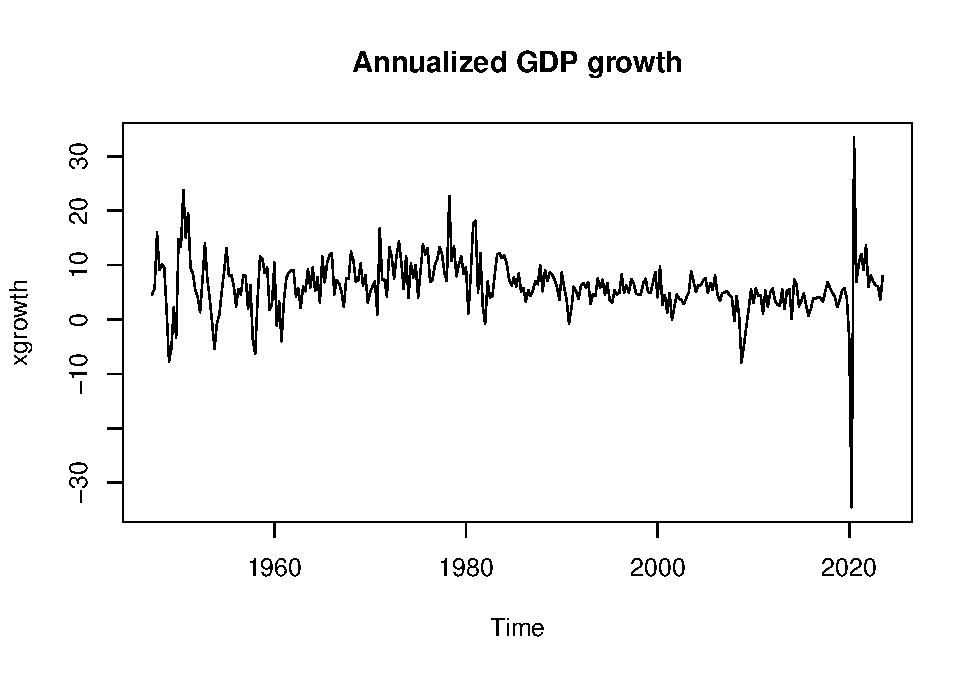
\includegraphics{_main_files/figure-latex/unnamed-chunk-9-1.pdf}

\hypertarget{empirical-moments-and-summary-statistics}{%
\section{Empirical moments and summary statistics}\label{empirical-moments-and-summary-statistics}}

For this example we use the \href{https://fred.stlouisfed.org/series/GDP}{U.S. GDP data}.

\begin{Shaded}
\begin{Highlighting}[]
\NormalTok{x }\OtherTok{\textless{}{-}} \FunctionTok{read.csv}\NormalTok{(}\StringTok{"../data/us{-}gdp.csv"}\NormalTok{)[,}\DecValTok{2}\NormalTok{]}
\NormalTok{x }\OtherTok{\textless{}{-}} \FunctionTok{ts}\NormalTok{(x, }\AttributeTok{start =} \FunctionTok{c}\NormalTok{(}\DecValTok{1947}\NormalTok{, }\DecValTok{1}\NormalTok{), }\AttributeTok{frequency =} \DecValTok{4}\NormalTok{)}
\NormalTok{t\_max }\OtherTok{\textless{}{-}} \FunctionTok{length}\NormalTok{(x)}
\FunctionTok{plot.ts}\NormalTok{(x, }\AttributeTok{main =} \StringTok{"U.S. GDP"}\NormalTok{, }\AttributeTok{ylab =} \StringTok{"Billions of dollars"}\NormalTok{)}
\end{Highlighting}
\end{Shaded}

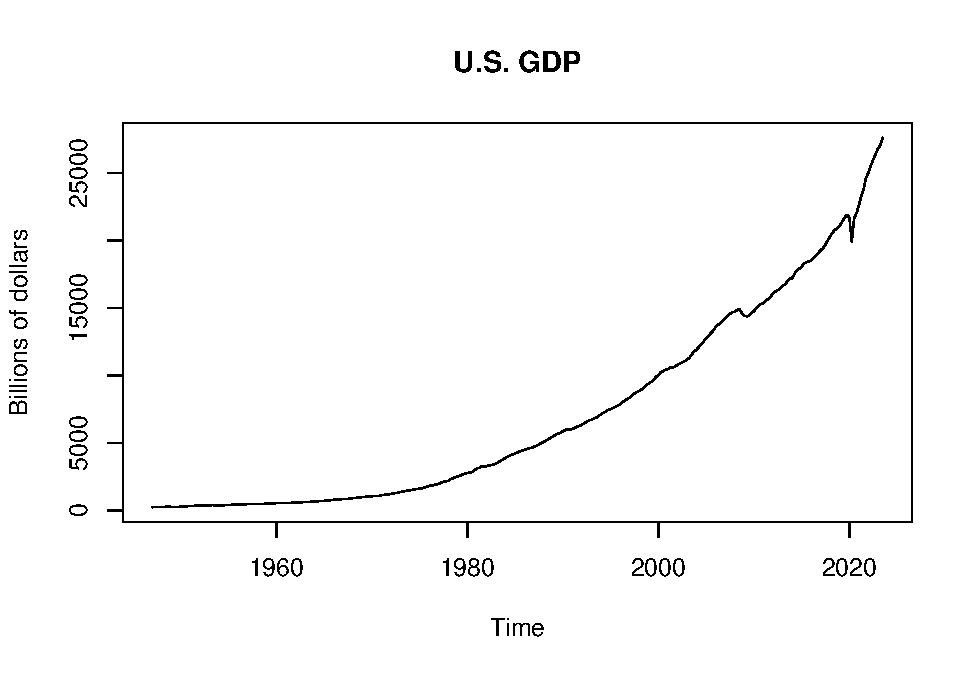
\includegraphics{_main_files/figure-latex/unnamed-chunk-10-1.pdf}

Consider the annualized quarterly growth rates:

\begin{Shaded}
\begin{Highlighting}[]
\CommentTok{\# xgrowth \textless{}{-} ( (x[2:t\_max]/x[1:(t\_max{-}1)])\^{}4 {-} 1 )*100}
\NormalTok{xgrowth }\OtherTok{\textless{}{-}} \DecValTok{4}\SpecialCharTok{*}\FunctionTok{diff}\NormalTok{(}\FunctionTok{log}\NormalTok{(x))}\SpecialCharTok{*}\DecValTok{100}
\NormalTok{xgrowth }\OtherTok{\textless{}{-}} \FunctionTok{ts}\NormalTok{(xgrowth, }\AttributeTok{start =} \FunctionTok{c}\NormalTok{(}\DecValTok{1947}\NormalTok{, }\DecValTok{2}\NormalTok{), }\AttributeTok{frequency =} \DecValTok{4}\NormalTok{)}
\FunctionTok{plot.ts}\NormalTok{(xgrowth, }\AttributeTok{main =} \StringTok{"Annualized GDP growth"}\NormalTok{)}
\end{Highlighting}
\end{Shaded}

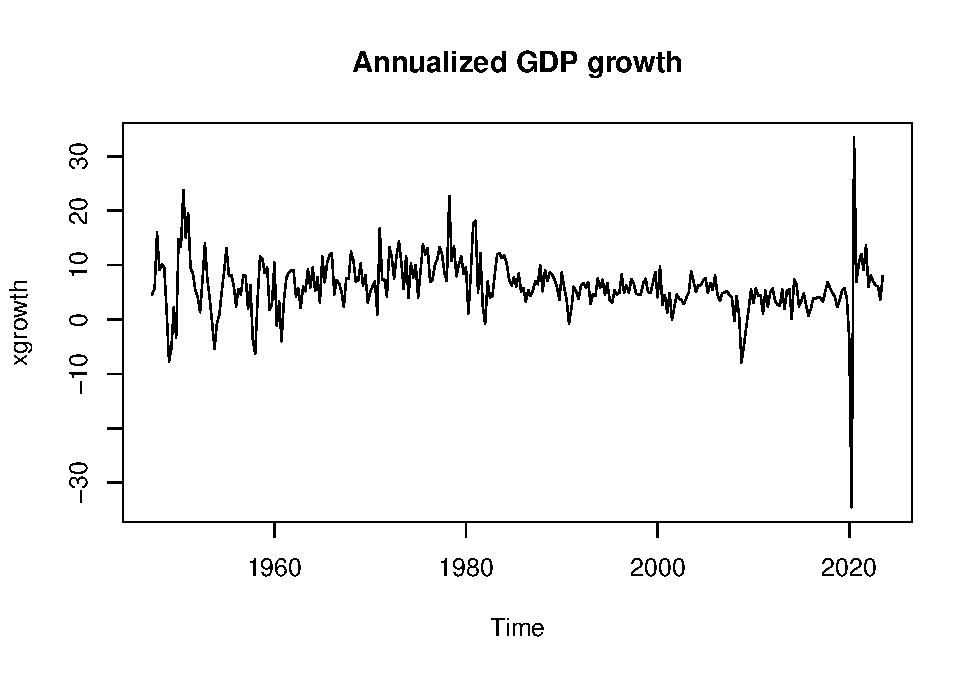
\includegraphics{_main_files/figure-latex/unnamed-chunk-11-1.pdf}

Below we compute some summary statistics for the time series of the U.S. GDP growth rates.

\begin{Shaded}
\begin{Highlighting}[]
\DocumentationTok{\#\# Example 4: empirical moments and summary statistics of the GDP growth}
\FunctionTok{library}\NormalTok{(moments)}
\FunctionTok{rbind}\NormalTok{(}
  \AttributeTok{mean     =} \FunctionTok{mean}\NormalTok{(xgrowth),}
  \AttributeTok{variance =} \FunctionTok{var}\NormalTok{(xgrowth),}
  \AttributeTok{skewness =} \FunctionTok{skewness}\NormalTok{(xgrowth),}
  \AttributeTok{kurtosis =} \FunctionTok{kurtosis}\NormalTok{(xgrowth),}
  \AttributeTok{min      =} \FunctionTok{min}\NormalTok{(xgrowth),}
  \AttributeTok{max      =} \FunctionTok{max}\NormalTok{(xgrowth),}
  \AttributeTok{above\_5  =} \FunctionTok{mean}\NormalTok{(xgrowth }\SpecialCharTok{\textgreater{}} \DecValTok{5}\NormalTok{),}
  \AttributeTok{annualized\_volatility =} \FunctionTok{sqrt}\NormalTok{(}\DecValTok{4}\NormalTok{)}\SpecialCharTok{*}\FunctionTok{sd}\NormalTok{(xgrowth)}
\NormalTok{)}
\end{Highlighting}
\end{Shaded}

\begin{verbatim}
##                              [,1]
## mean                    6.1858847
## variance               26.5117326
## skewness               -0.9793909
## kurtosis               17.9597257
## min                   -34.4929551
## max                    33.4065902
## above_5                 0.6078431
## annualized_volatility  10.2979090
\end{verbatim}

\begin{Shaded}
\begin{Highlighting}[]
\DocumentationTok{\#\# Autocovariance function}
\NormalTok{gamma }\OtherTok{\textless{}{-}} \ControlFlowTok{function}\NormalTok{(x, k) \{}
\NormalTok{  k }\OtherTok{\textless{}{-}} \FunctionTok{abs}\NormalTok{(k)}
\NormalTok{  t\_max }\OtherTok{\textless{}{-}} \FunctionTok{length}\NormalTok{(x)}
  \CommentTok{\# (t\_max{-}k)/t\_max * cov(x[1:(length(x){-}k)], x[(k+1):length(x)]) \# for compatibility with acf()}
  \FunctionTok{cov}\NormalTok{(x[}\DecValTok{1}\SpecialCharTok{:}\NormalTok{(t\_max}\SpecialCharTok{{-}}\NormalTok{k)], x[(k}\SpecialCharTok{+}\DecValTok{1}\NormalTok{)}\SpecialCharTok{:}\NormalTok{t\_max])}
\NormalTok{\}}

\DocumentationTok{\#\# Autocorrelation}
\NormalTok{rho }\OtherTok{\textless{}{-}} \ControlFlowTok{function}\NormalTok{(x, k) \{}\FunctionTok{gamma}\NormalTok{(x, k) }\SpecialCharTok{/} \FunctionTok{gamma}\NormalTok{(x, }\DecValTok{0}\NormalTok{)\}}

\DocumentationTok{\#\# autocorrelation at different lags}
\FunctionTok{sapply}\NormalTok{(}\DecValTok{0}\SpecialCharTok{:}\DecValTok{12}\NormalTok{, rho, }\AttributeTok{x =}\NormalTok{ xgrowth)}
\end{Highlighting}
\end{Shaded}

\begin{verbatim}
##  [1]  1.000000000  0.262228567  0.254514380  0.097922439  0.030475252
##  [6] -0.016390183 -0.003186283  0.054980002  0.062358818  0.146571003
## [11]  0.169620140  0.143289793  0.096325249
\end{verbatim}

Under the null hypothesis \(H_0: \rho = 0\), the sample autocorrelation is distributed as
\[
\sqrt{T} \ \hat{\rho} \xrightarrow{d} \mathcal{N}(0, 1)
\]

This means that the asymptotic variance of the estimator under the null is \(1/T\). The plot reports the 95\% confidence interval obtained as \(\left(0 \pm \frac{z_{0.975}}{\sqrt{T}}\right)\).

\begin{Shaded}
\begin{Highlighting}[]
\DocumentationTok{\#\# confidence interval}
\FunctionTok{qnorm}\NormalTok{(}\FloatTok{0.975}\NormalTok{)}\SpecialCharTok{*}\NormalTok{(}\DecValTok{1}\SpecialCharTok{/}\FunctionTok{sqrt}\NormalTok{(t\_max))}
\end{Highlighting}
\end{Shaded}

\begin{verbatim}
## [1] 0.1118611
\end{verbatim}

\begin{Shaded}
\begin{Highlighting}[]
\DocumentationTok{\#\# using built{-}in function for the autocorrelogram}
\FunctionTok{acf}\NormalTok{(xgrowth, }\AttributeTok{lag.max =} \DecValTok{16}\NormalTok{)}
\end{Highlighting}
\end{Shaded}

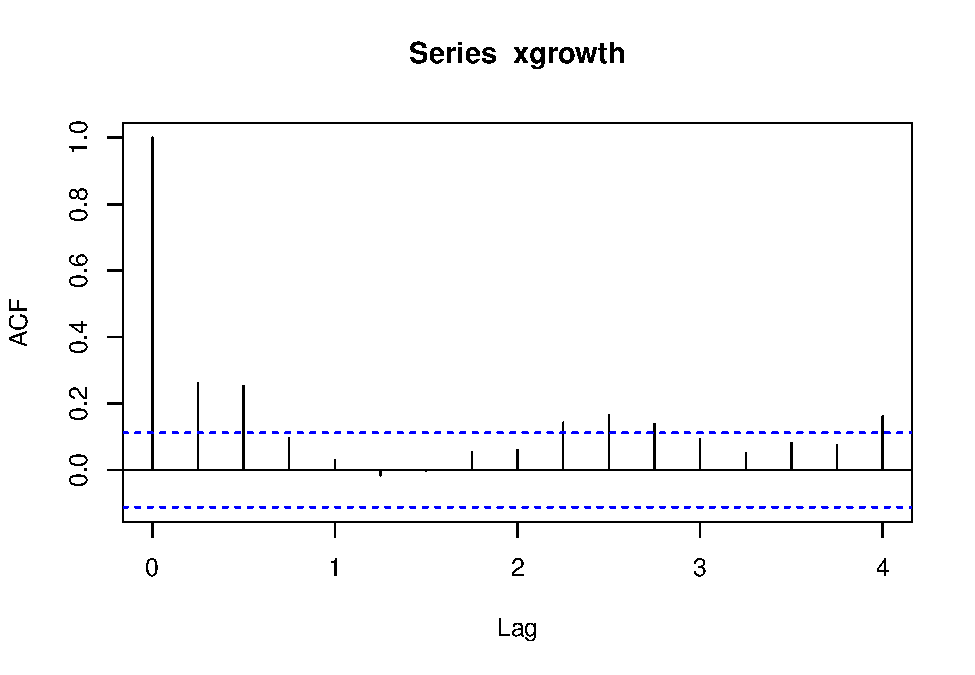
\includegraphics{_main_files/figure-latex/unnamed-chunk-15-1.pdf}

\begin{Shaded}
\begin{Highlighting}[]
\DocumentationTok{\#\# partial autocorrelation function}
\FunctionTok{pacf}\NormalTok{(xgrowth, }\AttributeTok{lag.max =} \DecValTok{16}\NormalTok{)}
\end{Highlighting}
\end{Shaded}

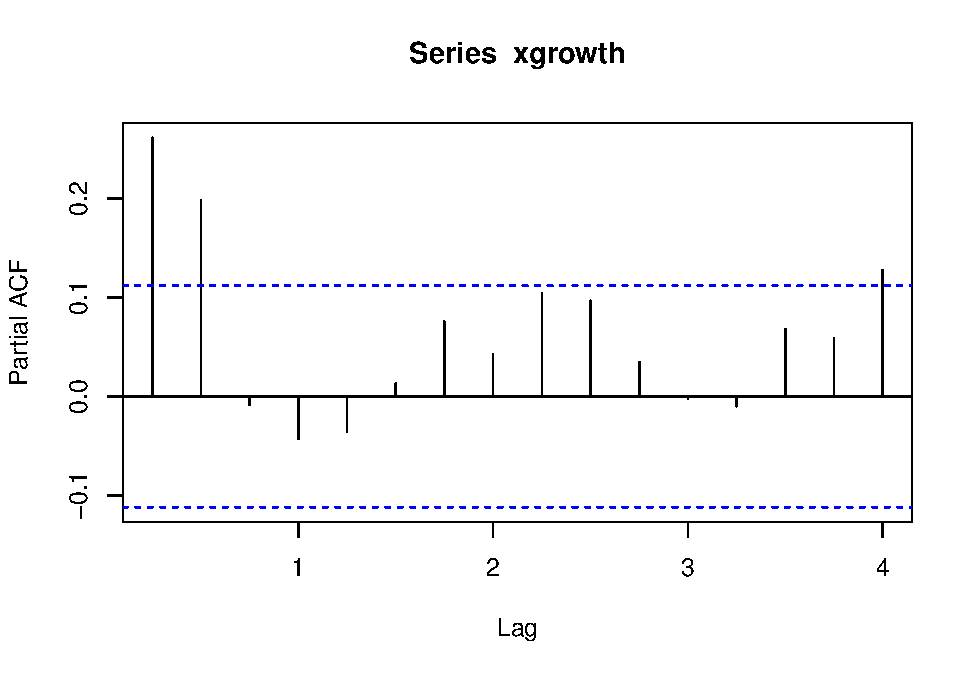
\includegraphics{_main_files/figure-latex/unnamed-chunk-16-1.pdf}

\hypertarget{hypothesis-testing}{%
\section{Hypothesis testing}\label{hypothesis-testing}}

In this section we use three testing procedures on the GDP growth data: the Augmented Dickey-Fuller test for stationarity, the Jarque-Bera test for normality and the t-test for the mean of a process.

\begin{Shaded}
\begin{Highlighting}[]
\DocumentationTok{\#\# Example 5: tests on GDP growth rates }
\FunctionTok{library}\NormalTok{(tseries)}

\DocumentationTok{\#\# stationarity: augmented Dickey{-}Fuller}
\FunctionTok{adf.test}\NormalTok{(x)}
\end{Highlighting}
\end{Shaded}

\begin{verbatim}
## 
##  Augmented Dickey-Fuller Test
## 
## data:  x
## Dickey-Fuller = 2.4611, Lag order = 6, p-value = 0.99
## alternative hypothesis: stationary
\end{verbatim}

\begin{Shaded}
\begin{Highlighting}[]
\FunctionTok{adf.test}\NormalTok{(xgrowth)}
\end{Highlighting}
\end{Shaded}

\begin{verbatim}
## 
##  Augmented Dickey-Fuller Test
## 
## data:  xgrowth
## Dickey-Fuller = -5.9064, Lag order = 6, p-value = 0.01
## alternative hypothesis: stationary
\end{verbatim}

\begin{Shaded}
\begin{Highlighting}[]
\DocumentationTok{\#\# normality: Jarque{-}Bera}
\FunctionTok{jarque.bera.test}\NormalTok{(xgrowth)}
\end{Highlighting}
\end{Shaded}

\begin{verbatim}
## 
##  Jarque Bera Test
## 
## data:  xgrowth
## X-squared = 2902.3, df = 2, p-value < 2.2e-16
\end{verbatim}

\begin{Shaded}
\begin{Highlighting}[]
\DocumentationTok{\#\# mean zero: t{-}test}
\NormalTok{sigmaLR }\OtherTok{\textless{}{-}} \FunctionTok{sum}\NormalTok{(}\FunctionTok{sapply}\NormalTok{(}\SpecialCharTok{{-}}\DecValTok{100}\SpecialCharTok{:}\DecValTok{100}\NormalTok{, gamma, }\AttributeTok{x =}\NormalTok{ xgrowth))}
\NormalTok{t\_stat  }\OtherTok{\textless{}{-}} \FunctionTok{mean}\NormalTok{(xgrowth)}\SpecialCharTok{/}\NormalTok{(}\FunctionTok{sqrt}\NormalTok{(sigmaLR}\SpecialCharTok{/}\NormalTok{t\_max))}
\NormalTok{p\_value }\OtherTok{\textless{}{-}}\NormalTok{ (}\DecValTok{1}\SpecialCharTok{{-}}\FunctionTok{pnorm}\NormalTok{(}\FunctionTok{abs}\NormalTok{(t\_stat)))}\SpecialCharTok{*}\DecValTok{2}
\CommentTok{\# plot(density(rnorm(1e6)), xlim = c({-}8, 8))}
\CommentTok{\# abline(v = t\_stat, col = "tomato", lwd = 2)}

\CommentTok{\# compare with unadjusted variance}
\CommentTok{\# t.test(xgrowth, mu = 0)}
\CommentTok{\# mean(xgrowth)/(sqrt((t\_max/(t\_max{-}1))*var(xgrowth)/t\_max)) \# for compatibility with t{-}test()}
\NormalTok{t\_stat\_unadjasted }\OtherTok{\textless{}{-}} \FunctionTok{mean}\NormalTok{(xgrowth)}\SpecialCharTok{/}\NormalTok{(}\FunctionTok{sqrt}\NormalTok{(}\FunctionTok{var}\NormalTok{(xgrowth)}\SpecialCharTok{/}\NormalTok{t\_max))}
\NormalTok{p\_value\_unadjasted }\OtherTok{\textless{}{-}}\NormalTok{ (}\DecValTok{1}\SpecialCharTok{{-}}\FunctionTok{pnorm}\NormalTok{(}\FunctionTok{abs}\NormalTok{(t\_stat\_unadjasted)))}\SpecialCharTok{*}\DecValTok{2}

\FunctionTok{rbind}\NormalTok{(}\AttributeTok{p\_value\_unadjasted =}\NormalTok{ p\_value\_unadjasted,}
      \AttributeTok{p\_value =}\NormalTok{ p\_value)}
\end{Highlighting}
\end{Shaded}

\begin{verbatim}
##                            [,1]
## p_value_unadjasted 0.000000e+00
## p_value            4.884981e-15
\end{verbatim}

\begin{Shaded}
\begin{Highlighting}[]
\CommentTok{\# We can study when does the adjustment really matters }
\CommentTok{\# using the results of the previous Monte Carlo simulation}

\DocumentationTok{\#\# Get variance and long{-}run variance}
\NormalTok{sigma }\OtherTok{\textless{}{-}} \FunctionTok{apply}\NormalTok{(x\_list, }\DecValTok{2}\NormalTok{, }\ControlFlowTok{function}\NormalTok{(x) }\FunctionTok{sqrt}\NormalTok{(}\FunctionTok{gamma}\NormalTok{(x, }\AttributeTok{k =} \DecValTok{0}\NormalTok{)}\SpecialCharTok{/}\FunctionTok{length}\NormalTok{(x)))}
\NormalTok{sigmaLR }\OtherTok{\textless{}{-}} \FunctionTok{apply}\NormalTok{(x\_list, }\DecValTok{2}\NormalTok{, }\ControlFlowTok{function}\NormalTok{(x) }\FunctionTok{sqrt}\NormalTok{(}\FunctionTok{sum}\NormalTok{(}\FunctionTok{sapply}\NormalTok{(}\SpecialCharTok{{-}}\DecValTok{3}\SpecialCharTok{:}\DecValTok{3}\NormalTok{, gamma, }\AttributeTok{x =}\NormalTok{ x))}\SpecialCharTok{/}\FunctionTok{length}\NormalTok{(x)))}

\DocumentationTok{\#\# Get adjusted and unadjusted t{-}statistics}
\NormalTok{t\_stat\_unadjasted }\OtherTok{\textless{}{-}}\NormalTok{ x\_means}\SpecialCharTok{/}\NormalTok{sigma}
\NormalTok{t\_stat }\OtherTok{\textless{}{-}}\NormalTok{ x\_means}\SpecialCharTok{/}\NormalTok{sigmaLR}

\DocumentationTok{\#\# Compute percentage of type{-}1 errors in the simulation}
\NormalTok{type1error }\OtherTok{\textless{}{-}} \FunctionTok{mean}\NormalTok{(}\FunctionTok{abs}\NormalTok{(t\_stat) }\SpecialCharTok{\textgreater{}} \FunctionTok{qnorm}\NormalTok{(}\FloatTok{0.975}\NormalTok{))}
\NormalTok{type1error\_unadjusted }\OtherTok{\textless{}{-}} \FunctionTok{mean}\NormalTok{(}\FunctionTok{abs}\NormalTok{(t\_stat\_unadjasted) }\SpecialCharTok{\textgreater{}} \FunctionTok{qnorm}\NormalTok{(}\FloatTok{0.975}\NormalTok{))}

\FunctionTok{rbind}\NormalTok{(}
  \AttributeTok{type1error =}\NormalTok{ type1error,}
  \AttributeTok{type1error\_unadjusted =}\NormalTok{ type1error\_unadjusted}
\NormalTok{)}
\end{Highlighting}
\end{Shaded}

\begin{verbatim}
##                         [,1]
## type1error            0.0569
## type1error_unadjusted 0.1716
\end{verbatim}

\begin{Shaded}
\begin{Highlighting}[]
\DocumentationTok{\#\# plot distributions of adjusted and unadjusted t{-}statistics}
\FunctionTok{hist}\NormalTok{(t\_stat\_unadjasted, }\AttributeTok{breaks =} \DecValTok{100}\NormalTok{, }\AttributeTok{freq =} \ConstantTok{FALSE}\NormalTok{, }\AttributeTok{col =} \StringTok{"tomato"}\NormalTok{, }
     \AttributeTok{ylim =} \FunctionTok{c}\NormalTok{(}\DecValTok{0}\NormalTok{, }\FloatTok{0.45}\NormalTok{), }\AttributeTok{xlim =} \FunctionTok{c}\NormalTok{(}\SpecialCharTok{{-}}\DecValTok{5}\NormalTok{, }\DecValTok{6}\NormalTok{), }\AttributeTok{xlab =} \StringTok{"t{-}stat"}\NormalTok{, }
     \AttributeTok{main =} \StringTok{"Distribution of the t{-}statistic in Monte Carlo simulation"}\NormalTok{)}
\FunctionTok{hist}\NormalTok{(t\_stat, }\AttributeTok{breaks =} \DecValTok{100}\NormalTok{, }\AttributeTok{freq =} \ConstantTok{FALSE}\NormalTok{, }\AttributeTok{add =} \ConstantTok{TRUE}\NormalTok{, }\AttributeTok{col =} \StringTok{"lightgreen"}\NormalTok{)}
\FunctionTok{lines}\NormalTok{(}\FunctionTok{density}\NormalTok{(}\FunctionTok{rnorm}\NormalTok{(}\FloatTok{1e6}\NormalTok{, }\AttributeTok{mean =} \DecValTok{0}\NormalTok{, }\AttributeTok{sd =} \DecValTok{1}\NormalTok{)), }\AttributeTok{lwd =} \DecValTok{4}\NormalTok{, }\AttributeTok{col =} \StringTok{"black"}\NormalTok{)}
\FunctionTok{legend}\NormalTok{(}\StringTok{"topright"}\NormalTok{, }\FunctionTok{c}\NormalTok{(}\StringTok{"Unadjusted"}\NormalTok{, }\StringTok{"Adjusted"}\NormalTok{), }\AttributeTok{col=}\FunctionTok{c}\NormalTok{(}\StringTok{"tomato"}\NormalTok{, }\StringTok{"lightgreen"}\NormalTok{), }\AttributeTok{lwd=}\DecValTok{6}\NormalTok{)}
\FunctionTok{abline}\NormalTok{(}\AttributeTok{v =} \FunctionTok{qnorm}\NormalTok{(}\FunctionTok{c}\NormalTok{(}\FloatTok{0.025}\NormalTok{, }\FloatTok{0.975}\NormalTok{)), }\AttributeTok{lty =} \DecValTok{2}\NormalTok{, }\AttributeTok{lwd =} \DecValTok{2}\NormalTok{)}
\FunctionTok{text}\NormalTok{(}\AttributeTok{x=}\FunctionTok{c}\NormalTok{(}\FloatTok{6.5}\NormalTok{, }\FloatTok{6.5}\NormalTok{), }\AttributeTok{y=}\FunctionTok{c}\NormalTok{(}\FloatTok{0.3}\NormalTok{, }\FloatTok{0.25}\NormalTok{), }
     \AttributeTok{labels=}\FunctionTok{c}\NormalTok{(}\FunctionTok{paste0}\NormalTok{(}\StringTok{"Type 1 error: "}\NormalTok{, }\FunctionTok{round}\NormalTok{(type1error\_unadjusted}\SpecialCharTok{*}\DecValTok{100}\NormalTok{, }\DecValTok{1}\NormalTok{), }\StringTok{"\%"}\NormalTok{),}
              \FunctionTok{paste0}\NormalTok{(}\StringTok{"Type 1 error adjusted: "}\NormalTok{, }\FunctionTok{round}\NormalTok{(type1error}\SpecialCharTok{*}\DecValTok{100}\NormalTok{, }\DecValTok{1}\NormalTok{), }\StringTok{"\%"}\NormalTok{)), }
     \AttributeTok{col=}\FunctionTok{c}\NormalTok{(}\StringTok{"tomato"}\NormalTok{, }\StringTok{"lightgreen"}\NormalTok{), }\AttributeTok{pos =} \DecValTok{2}\NormalTok{)}
\end{Highlighting}
\end{Shaded}

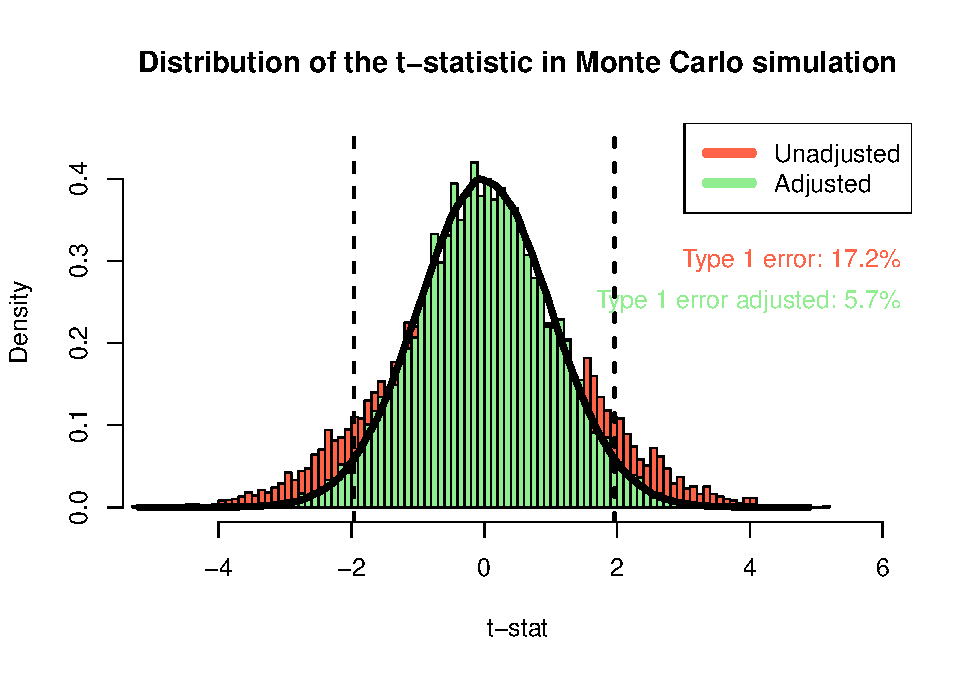
\includegraphics{_main_files/figure-latex/unnamed-chunk-19-1.pdf}

\hypertarget{session02}{%
\chapter{Forecasting with time-series regression}\label{session02}}

This session covers a first introduction to forecasting the conditional mean of a time series. A forecasting procedure involves three main objects:

\begin{itemize}
\tightlist
\item
  A set of predictors and a target variable that we want to forecast
\item
  A class of forecasting models that we consider
\item
  A loss function to evaluate the accuracy of the forecasts
\end{itemize}

In this session we focus on the class of linear regression models estimated via least-squares. The loss function that we consider throughout this chapter is the quadratic loss function estimated using the Mean Squared Error (MSE) defined in the \texttt{R} function below.

\begin{Shaded}
\begin{Highlighting}[]
\DocumentationTok{\#\# Function to compute the MSE. y = true value, f = forecast}
\NormalTok{mse }\OtherTok{\textless{}{-}} \ControlFlowTok{function}\NormalTok{(y, f) \{}\FunctionTok{mean}\NormalTok{((y}\SpecialCharTok{{-}}\NormalTok{f)}\SpecialCharTok{\^{}}\DecValTok{2}\NormalTok{)\}}
\end{Highlighting}
\end{Shaded}

The first section presents a simulation exercise to show the finite-sample properties of the linear regression model under mis-specification. The second section is an empirical application to the problem of forecasting the U.S. unemployment rate using some relevant macroeconomic indicators.

\hypertarget{oracle-inequality}{%
\section{Oracle inequality}\label{oracle-inequality}}

\textbf{Optional section, not covered in class}

Given a forecasting problem, the optimal prediction rule is defined as the one that minimizes the theoretical risk:
\[
f_{t+h|t}^* = \arg\min_{f \in \mathcal{F}} R(f_{t+h|t}) 
\]

and the associated optimal risk is denoted by \(R^*\). Under the square loss function, the optimal rule is the conditional expectation:

\[
f_{t+h|t}^* = \mathbb{E}[y_{t+h}| x_t]
\]

Notice that the exact functional form of the predictor is unknown: the conditional expected value could be of any linear or non-linear form. To make the theory of learning operational, we then have to restrict our attention to a class of prediction rules and pick the best rule from that class according to the limited amount of data available.

A commonly used class of predictors is that of the linear predictors. Consider a linear regression model for predicting the target variable \(y_{t+h}\):
\[
f_{t+h|t} = x_t'\theta.
\]

where \(f_{t+h|t}\) denotes the \(h\)-periods-ahead forecast. Irrespective of what is the true d.g.p., \(\theta\) is the parameter that leads to the best forecasts \emph{within the class of linear regression models}

\[
\theta = \arg\min_{\tilde{\theta} \in \mathbb{R}^p} \mathbb{E}[L(y_{t+h}, f_{t+h|t}(\theta))] = R(\theta)
\]

However, in practice we can only use a finite sample to learn the parameters of the linear model via \emph{empirical} risk minimization:

\[
\hat{\theta} = \arg\min_{\theta \in \mathbb{R}^p} R_T(\theta)
\]

In our case, \(R_T(\theta) = \frac{1}{T-h-t_w+1}\sum_{t=t_w}^{T-h} (y_{t+h} - f_{t+h|t})^2 = MSE\), where \(t_w\) denotes the initial number of observations used to train the model.

So far, we have introduced three different measures of risk:

\begin{itemize}
\tightlist
\item
  \(R^*\), the risk associated with the theoretical optimal predictor if the true d.g.p. were known
\item
  \(R(\theta)\), the risk associated with the optimal predictor within the parametric class considered for learning
\item
  \(R_T(\hat\theta)\), the empirical risk obtained by minimization of the loss function using the available data sample
\end{itemize}

The regret (i.e.~the difference between the optimal and the empirical risk) can be expressed in a way that links these three quantities:
\[
 R_T(\hat\theta) - R^*  = \underbrace{\left[ R(\theta) - R^* \right]}_{_{\text{Approximation error}}} + \underbrace{\left[R_T(\hat\theta) - R(\theta)\right]}_{\text{Estimation error}}
 \]

We mainly focus on the estimation error. In particular, we are usually interested in establishing finite-sample, probabilistic bounds to this quantity. These bounds are helpful in assessing, for instance, how many observations a model needs to perform well and how its performance relates to the number of predictors. For linear prediction, the following oracle inequality holds: there exists a constant \(c\) such that

\[
R(\hat\theta) \leq R(\theta) + c \frac{p}{T}, \quad \text{w.p. } 1-1/T 
\]

The example below shows that the inequality holds in a simulation setting. We generate \(10^6\) observations from the following process:

\[
y_t = 0.6\times y_{t-1} - \tanh(0.3 \times y_{t-1}) + 
              0.8\times x_{1,t-1} + 0.2 \times x_{2,t-1} -
              0.7\times x_{3,t-1} + \varepsilon_t, 
\]

where \(\varepsilon_t \sim \mathcal{N}(0, 0.5)\) and the variables \(x_{1,t}, x_{2,t}, x_{3,t}\) are drawn independently from a standard normal distribution. We then consider the class of linear regression models,

\[
y_t = \beta_0 + \beta_1 y_{t-1} + \beta_2 x_{1,t-1} + \beta_3 x_{2,t-1} + \beta_3 x_{3,t-1} + u_t
\]

Notice that the OLS estimator is the empirical risk minimizer in the case of a square loss. In the simulation setting, we can also obtain \(R(\theta)\) by estimating the parameters of the regression using the entire simulated population. We can then draw many estimates of \(R(\hat\theta)\) by considering different subsamples of the simulated population and estimating the parameters of the model using OLS on the subsample. By doing so, we can simulate the distribution of the empirical risk and compare it against the overall minimum risk within the class of linear estimators to assess the oracle inequality. We repeat the exercise considering different sizes of the subsamples to show that the bound gets tighter as the sample size increases, as it must be for the inequality to have the oracle property.

\begin{Shaded}
\begin{Highlighting}[]
\DocumentationTok{\#\# Example 1: simulation for oracle inequality}
\CommentTok{\# build the simulated population dataset}
\NormalTok{N }\OtherTok{\textless{}{-}} \DecValTok{3}
\NormalTok{T\_pop }\OtherTok{\textless{}{-}} \FloatTok{1e5}

\FunctionTok{set.seed}\NormalTok{(}\DecValTok{455}\NormalTok{)}
\NormalTok{x\_pop }\OtherTok{\textless{}{-}} \FunctionTok{matrix}\NormalTok{(}\FunctionTok{rnorm}\NormalTok{((T\_pop}\SpecialCharTok{+}\DecValTok{1}\NormalTok{)}\SpecialCharTok{*}\NormalTok{N), }\AttributeTok{ncol =}\NormalTok{ N)}
\NormalTok{y\_pop }\OtherTok{\textless{}{-}} \FunctionTok{rep}\NormalTok{(}\DecValTok{0}\NormalTok{, T\_pop)}
\ControlFlowTok{for}\NormalTok{ (t }\ControlFlowTok{in} \DecValTok{2}\SpecialCharTok{:}\NormalTok{(T\_pop}\SpecialCharTok{+}\DecValTok{1}\NormalTok{)) \{}
  \FunctionTok{set.seed}\NormalTok{(}\DecValTok{456}\SpecialCharTok{*}\NormalTok{t)}
  \CommentTok{\# non{-}linear d.g.p.}
\NormalTok{  y\_pop[t] }\OtherTok{\textless{}{-}} \FloatTok{0.6}\SpecialCharTok{*}\NormalTok{y\_pop[t}\DecValTok{{-}1}\NormalTok{] }\SpecialCharTok{{-}} \FunctionTok{tanh}\NormalTok{(}\FloatTok{0.3}\SpecialCharTok{*}\NormalTok{y\_pop[t}\DecValTok{{-}1}\NormalTok{]) }\SpecialCharTok{+} 
              \FloatTok{0.8}\SpecialCharTok{*}\NormalTok{x\_pop[t}\DecValTok{{-}1}\NormalTok{, }\DecValTok{1}\NormalTok{] }\SpecialCharTok{+} \FloatTok{0.2}\SpecialCharTok{*}\NormalTok{x\_pop[t}\DecValTok{{-}1}\NormalTok{, }\DecValTok{2}\NormalTok{] }\SpecialCharTok{{-}}
              \FloatTok{0.7}\SpecialCharTok{*}\NormalTok{x\_pop[t}\DecValTok{{-}1}\NormalTok{, }\DecValTok{3}\NormalTok{] }\SpecialCharTok{+} \FunctionTok{rnorm}\NormalTok{(}\DecValTok{1}\NormalTok{, }\AttributeTok{sd =} \FloatTok{0.5}\NormalTok{)}
\NormalTok{\}}
\FunctionTok{colnames}\NormalTok{(x\_pop) }\OtherTok{\textless{}{-}} \FunctionTok{paste0}\NormalTok{(}\StringTok{"x"}\NormalTok{, }\DecValTok{1}\SpecialCharTok{:}\NormalTok{N)}

\CommentTok{\# target is y(t+1). predictor is x(t)}
\NormalTok{d\_pop }\OtherTok{\textless{}{-}} \FunctionTok{as.data.frame}\NormalTok{(}\FunctionTok{cbind}\NormalTok{(}\AttributeTok{y =}\NormalTok{ y\_pop[}\DecValTok{2}\SpecialCharTok{:}\NormalTok{(T\_pop}\SpecialCharTok{+}\DecValTok{1}\NormalTok{)] , x\_pop[}\DecValTok{1}\SpecialCharTok{:}\NormalTok{T\_pop,] ))}
\end{Highlighting}
\end{Shaded}

\begin{Shaded}
\begin{Highlighting}[]
\CommentTok{\# estimate the linear predictor y(t) = x(t{-}1)\textquotesingle{}b via OLS}
\NormalTok{model\_pop }\OtherTok{\textless{}{-}} \FunctionTok{lm}\NormalTok{(y }\SpecialCharTok{\textasciitilde{}}\NormalTok{ x1 }\SpecialCharTok{+}\NormalTok{ x2 }\SpecialCharTok{+}\NormalTok{ x3, }\AttributeTok{data =}\NormalTok{ d\_pop)}
\FunctionTok{summary}\NormalTok{(model\_pop)}
\end{Highlighting}
\end{Shaded}

\begin{Shaded}
\begin{Highlighting}[]
\DocumentationTok{\#\# estimate the optimal risk and the population risk within the linear family}
\CommentTok{\# optimal}
\NormalTok{f\_optimal }\OtherTok{\textless{}{-}} \FunctionTok{rep}\NormalTok{(}\ConstantTok{NA}\NormalTok{, T\_pop}\SpecialCharTok{+}\DecValTok{1}\NormalTok{)}
\ControlFlowTok{for}\NormalTok{ (t }\ControlFlowTok{in} \DecValTok{1}\SpecialCharTok{:}\NormalTok{T\_pop) \{}
\NormalTok{  f\_optimal[t}\SpecialCharTok{+}\DecValTok{1}\NormalTok{] }\OtherTok{\textless{}{-}} \FloatTok{0.6}\SpecialCharTok{*}\NormalTok{y\_pop[t] }\SpecialCharTok{{-}} \FunctionTok{tanh}\NormalTok{(}\FloatTok{0.3}\SpecialCharTok{*}\NormalTok{y\_pop[t]) }\SpecialCharTok{+} 
                    \FloatTok{0.8}\SpecialCharTok{*}\NormalTok{x\_pop[t, }\DecValTok{1}\NormalTok{] }\SpecialCharTok{+} \FloatTok{0.2}\SpecialCharTok{*}\NormalTok{x\_pop[t, }\DecValTok{2}\NormalTok{] }\SpecialCharTok{{-}}
                    \FloatTok{0.7}\SpecialCharTok{*}\NormalTok{x\_pop[t, }\DecValTok{3}\NormalTok{] }
\NormalTok{\}}
\NormalTok{f\_optimal }\OtherTok{\textless{}{-}}\NormalTok{ f\_optimal[}\SpecialCharTok{{-}}\DecValTok{1}\NormalTok{]}
\NormalTok{risk\_star }\OtherTok{\textless{}{-}} \FunctionTok{mse}\NormalTok{(d\_pop[,}\DecValTok{1}\NormalTok{], f\_optimal)}

\CommentTok{\# linear family}
\NormalTok{risk\_pop  }\OtherTok{\textless{}{-}} \FunctionTok{mse}\NormalTok{(d\_pop[,}\DecValTok{1}\NormalTok{], }\FunctionTok{predict}\NormalTok{(model\_pop))}
\end{Highlighting}
\end{Shaded}

\begin{Shaded}
\begin{Highlighting}[]
\DocumentationTok{\#\# Run the simulations to estimate a small{-}sample model many times}
\NormalTok{t\_small  }\OtherTok{\textless{}{-}} \DecValTok{30}
\NormalTok{t\_medium }\OtherTok{\textless{}{-}} \DecValTok{300}
\NormalTok{t\_large  }\OtherTok{\textless{}{-}} \DecValTok{3000}
\NormalTok{nsim }\OtherTok{\textless{}{-}} \DecValTok{1000}

\NormalTok{empirical\_risk }\OtherTok{\textless{}{-}} \FunctionTok{list}\NormalTok{(}
  \AttributeTok{model\_small =} \FunctionTok{rep}\NormalTok{(}\ConstantTok{NA}\NormalTok{, nsim),}
  \AttributeTok{model\_medium =} \FunctionTok{rep}\NormalTok{(}\ConstantTok{NA}\NormalTok{, nsim),}
  \AttributeTok{model\_large =} \FunctionTok{rep}\NormalTok{(}\ConstantTok{NA}\NormalTok{, nsim)}
\NormalTok{)}

\ControlFlowTok{for}\NormalTok{ (s }\ControlFlowTok{in} \DecValTok{1}\SpecialCharTok{:}\NormalTok{nsim) \{}
  \FunctionTok{set.seed}\NormalTok{(}\DecValTok{456}\SpecialCharTok{*}\NormalTok{s)}
  \CommentTok{\# pick index at random between 1e5 and 9e5}
\NormalTok{  idx }\OtherTok{\textless{}{-}} \FunctionTok{sample}\NormalTok{(}\DecValTok{1}\SpecialCharTok{:}\NormalTok{(T\_pop}\SpecialCharTok{{-}}\NormalTok{t\_large), }\DecValTok{1}\NormalTok{)}
  \CommentTok{\# consider the t subsequent observations}
\NormalTok{  d\_small  }\OtherTok{\textless{}{-}}\NormalTok{ d\_pop[idx}\SpecialCharTok{:}\NormalTok{(idx}\SpecialCharTok{+}\NormalTok{t\_small), ]}
\NormalTok{  d\_medium }\OtherTok{\textless{}{-}}\NormalTok{ d\_pop[idx}\SpecialCharTok{:}\NormalTok{(idx}\SpecialCharTok{+}\NormalTok{t\_medium),]}
\NormalTok{  d\_large  }\OtherTok{\textless{}{-}}\NormalTok{ d\_pop[idx}\SpecialCharTok{:}\NormalTok{(idx}\SpecialCharTok{+}\NormalTok{t\_large), ]}
  \CommentTok{\# estimate the model}
\NormalTok{  model\_small }\OtherTok{\textless{}{-}} \FunctionTok{lm}\NormalTok{(y }\SpecialCharTok{\textasciitilde{}}\NormalTok{ x1 }\SpecialCharTok{+}\NormalTok{ x2 }\SpecialCharTok{+}\NormalTok{ x3, }\AttributeTok{data =}\NormalTok{ d\_small)}
\NormalTok{  model\_medium }\OtherTok{\textless{}{-}} \FunctionTok{lm}\NormalTok{(y }\SpecialCharTok{\textasciitilde{}}\NormalTok{ x1 }\SpecialCharTok{+}\NormalTok{ x2 }\SpecialCharTok{+}\NormalTok{ x3, }\AttributeTok{data =}\NormalTok{ d\_medium)}
\NormalTok{  model\_large }\OtherTok{\textless{}{-}} \FunctionTok{lm}\NormalTok{(y }\SpecialCharTok{\textasciitilde{}}\NormalTok{ x1 }\SpecialCharTok{+}\NormalTok{ x2 }\SpecialCharTok{+}\NormalTok{ x3, }\AttributeTok{data =}\NormalTok{ d\_large)}
  \CommentTok{\# compute the MSE and store the results}
\NormalTok{  empirical\_risk}\SpecialCharTok{$}\NormalTok{model\_small[s] }\OtherTok{\textless{}{-}} \FunctionTok{mse}\NormalTok{(d\_small[,}\DecValTok{1}\NormalTok{], }\FunctionTok{predict}\NormalTok{(model\_small))}
\NormalTok{  empirical\_risk}\SpecialCharTok{$}\NormalTok{model\_medium[s] }\OtherTok{\textless{}{-}} \FunctionTok{mse}\NormalTok{(d\_medium[,}\DecValTok{1}\NormalTok{], }\FunctionTok{predict}\NormalTok{(model\_medium))}
\NormalTok{  empirical\_risk}\SpecialCharTok{$}\NormalTok{model\_large[s] }\OtherTok{\textless{}{-}} \FunctionTok{mse}\NormalTok{(d\_large[,}\DecValTok{1}\NormalTok{], }\FunctionTok{predict}\NormalTok{(model\_large))}
\NormalTok{\}}

\CommentTok{\# compute the constant C s.t. the bound risk\_pop + C(P/t) is satisfied}
\CommentTok{\# 1{-}1/t fraction of times}
\NormalTok{c\_small }\OtherTok{\textless{}{-}} \FunctionTok{quantile}\NormalTok{(empirical\_risk}\SpecialCharTok{$}\NormalTok{model\_small, }\DecValTok{1{-}1}\SpecialCharTok{/}\NormalTok{t\_small)}
\NormalTok{c\_medium }\OtherTok{\textless{}{-}} \FunctionTok{quantile}\NormalTok{(empirical\_risk}\SpecialCharTok{$}\NormalTok{model\_medium, }\DecValTok{1{-}1}\SpecialCharTok{/}\NormalTok{t\_medium)}
\NormalTok{c\_large }\OtherTok{\textless{}{-}} \FunctionTok{quantile}\NormalTok{(empirical\_risk}\SpecialCharTok{$}\NormalTok{model\_large, }\DecValTok{1{-}1}\SpecialCharTok{/}\NormalTok{t\_large)}
\end{Highlighting}
\end{Shaded}

\begin{Shaded}
\begin{Highlighting}[]
\DocumentationTok{\#\# report the distribution of the simulated empirical risks }
\FunctionTok{par}\NormalTok{(}\AttributeTok{mfrow =} \FunctionTok{c}\NormalTok{(}\DecValTok{2}\NormalTok{,}\DecValTok{2}\NormalTok{))}
\CommentTok{\# small}
\FunctionTok{hist}\NormalTok{(empirical\_risk}\SpecialCharTok{$}\NormalTok{model\_small, }\AttributeTok{xlab =} \StringTok{"Empirical risk"}\NormalTok{, }\AttributeTok{main =} \StringTok{"Small model"}\NormalTok{)}
\FunctionTok{abline}\NormalTok{(}\AttributeTok{v =}\NormalTok{ c\_small, }\AttributeTok{lwd =} \DecValTok{2}\NormalTok{, }\AttributeTok{lty =} \DecValTok{2}\NormalTok{)}
\FunctionTok{abline}\NormalTok{(}\AttributeTok{v =}\NormalTok{ risk\_pop, }\AttributeTok{lwd =} \DecValTok{3}\NormalTok{, }\AttributeTok{lty =} \DecValTok{1}\NormalTok{, }\AttributeTok{col =} \StringTok{"darkred"}\NormalTok{)}
\FunctionTok{text}\NormalTok{(}\AttributeTok{x =}\NormalTok{ c\_small}\SpecialCharTok{*}\FloatTok{1.2}\NormalTok{, }\AttributeTok{y =} \DecValTok{250}\NormalTok{, }\AttributeTok{labels =} \FunctionTok{paste0}\NormalTok{(}\StringTok{"Estimation error}\SpecialCharTok{\textbackslash{}n}\StringTok{bound: "}\NormalTok{, }
                                               \FunctionTok{round}\NormalTok{(c\_small}\SpecialCharTok{*}\NormalTok{N}\SpecialCharTok{/}\NormalTok{t\_small,}\DecValTok{3}\NormalTok{)))}
\CommentTok{\# medium}
\FunctionTok{hist}\NormalTok{(empirical\_risk}\SpecialCharTok{$}\NormalTok{model\_medium, }\AttributeTok{xlab =} \StringTok{"Empirical risk"}\NormalTok{, }\AttributeTok{main =} \StringTok{"Medium model"}\NormalTok{)}
\FunctionTok{abline}\NormalTok{(}\AttributeTok{v =}\NormalTok{ c\_medium, }\AttributeTok{lwd =} \DecValTok{2}\NormalTok{, }\AttributeTok{lty =} \DecValTok{2}\NormalTok{)}
\FunctionTok{abline}\NormalTok{(}\AttributeTok{v =}\NormalTok{ risk\_pop, }\AttributeTok{lwd =} \DecValTok{3}\NormalTok{, }\AttributeTok{lty =} \DecValTok{1}\NormalTok{, }\AttributeTok{col =} \StringTok{"darkred"}\NormalTok{)}
\FunctionTok{text}\NormalTok{(}\AttributeTok{x =}\NormalTok{ c\_medium}\SpecialCharTok{*}\FloatTok{0.98}\NormalTok{, }\AttributeTok{y =} \DecValTok{150}\NormalTok{, }\AttributeTok{labels =} \FunctionTok{paste0}\NormalTok{(}\StringTok{"Estimation error}\SpecialCharTok{\textbackslash{}n}\StringTok{bound: "}\NormalTok{, }
                                                \FunctionTok{round}\NormalTok{(c\_medium}\SpecialCharTok{*}\NormalTok{N}\SpecialCharTok{/}\NormalTok{t\_medium,}\DecValTok{3}\NormalTok{)))}
\CommentTok{\# large}
\FunctionTok{hist}\NormalTok{(empirical\_risk}\SpecialCharTok{$}\NormalTok{model\_large, }\AttributeTok{xlab =} \StringTok{"Empirical risk"}\NormalTok{, }\AttributeTok{main =} \StringTok{"Large model"}\NormalTok{)}
\FunctionTok{abline}\NormalTok{(}\AttributeTok{v =}\NormalTok{ c\_large, }\AttributeTok{lwd =} \DecValTok{2}\NormalTok{, }\AttributeTok{lty =} \DecValTok{2}\NormalTok{)}
\FunctionTok{abline}\NormalTok{(}\AttributeTok{v =}\NormalTok{ risk\_pop, }\AttributeTok{lwd =} \DecValTok{3}\NormalTok{, }\AttributeTok{lty =} \DecValTok{1}\NormalTok{, }\AttributeTok{col =} \StringTok{"darkred"}\NormalTok{)}
\FunctionTok{text}\NormalTok{(}\AttributeTok{x =}\NormalTok{ c\_large}\SpecialCharTok{*}\FloatTok{0.98}\NormalTok{, }\AttributeTok{y =} \DecValTok{120}\NormalTok{, }\AttributeTok{labels =} \FunctionTok{paste0}\NormalTok{(}\StringTok{"Estimation error}\SpecialCharTok{\textbackslash{}n}\StringTok{bound: "}\NormalTok{,}
                                               \FunctionTok{round}\NormalTok{(c\_large}\SpecialCharTok{*}\NormalTok{N}\SpecialCharTok{/}\NormalTok{t\_large,}\DecValTok{3}\NormalTok{)))}
\end{Highlighting}
\end{Shaded}

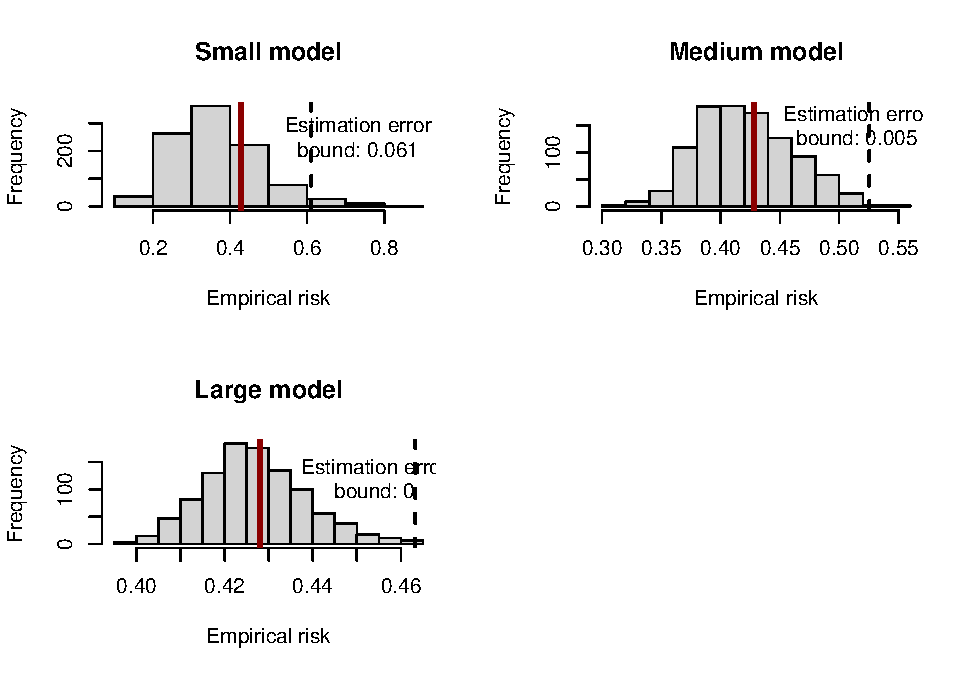
\includegraphics{_main_files/figure-latex/unnamed-chunk-26-1.pdf}

\hypertarget{application-forecasting-unemployment}{%
\section{Application: forecasting unemployment}\label{application-forecasting-unemployment}}

\begin{Shaded}
\begin{Highlighting}[]
\FunctionTok{library}\NormalTok{(sandwich) }\CommentTok{\# for estimation of robust standard errors}
\FunctionTok{library}\NormalTok{(lmtest)   }\CommentTok{\# for coeftest}
\FunctionTok{library}\NormalTok{(forecast) }\CommentTok{\# for dm.test}
\end{Highlighting}
\end{Shaded}

We now consider an empirical application using the U.S. data from the \href{https://research.stlouisfed.org/econ/mccracken/fred-databases/}{FRED-MD dataset}, a collection of 127 macroeconomic time series observed at a monthly frequency.
To make sure that the series in the model are stationary, we transform the variables according to the recommendation of the authors, as summarised in the transformation code \texttt{tcode} in the first row of the dataset:

\begin{longtable}[]{@{}ll@{}}
\toprule\noalign{}
\texttt{tcode} & Transformation \\
\midrule\noalign{}
\endhead
\bottomrule\noalign{}
\endlastfoot
1 & No \\
2 & \(\Delta x_t\) \\
3 & \(\Delta^2 x_t\) \\
4 & \(\log(x_t)\) \\
5 & \(\Delta\log(x_t)\) \\
6 & \(\Delta^2\log(x_t)\) \\
7 & \(\Delta\left(\frac{x_t}{x_{t-1}} -1 \right)\) \\
\end{longtable}

\begin{Shaded}
\begin{Highlighting}[]
\DocumentationTok{\#\# load FRED{-}MD data }
\NormalTok{fredmd }\OtherTok{\textless{}{-}} \FunctionTok{read.csv}\NormalTok{(}\StringTok{"../data/current.csv"}\NormalTok{)}
\NormalTok{dates  }\OtherTok{\textless{}{-}} \FunctionTok{as.Date}\NormalTok{(fredmd}\SpecialCharTok{$}\NormalTok{sasdate[}\SpecialCharTok{{-}}\DecValTok{1}\NormalTok{],}\StringTok{\textquotesingle{}\%m/\%d/\%Y\textquotesingle{}}\NormalTok{)}
\NormalTok{tcodes }\OtherTok{\textless{}{-}}\NormalTok{ fredmd[}\DecValTok{1}\NormalTok{,}\SpecialCharTok{{-}}\DecValTok{1}\NormalTok{]}
\NormalTok{d      }\OtherTok{\textless{}{-}}\NormalTok{ fredmd[}\SpecialCharTok{{-}}\DecValTok{1}\NormalTok{,}\SpecialCharTok{{-}}\DecValTok{1}\NormalTok{] }

\CommentTok{\# subset 1980{-}2024 period}
\NormalTok{data  }\OtherTok{\textless{}{-}}\NormalTok{ d[dates }\SpecialCharTok{\textgreater{}=} \StringTok{\textquotesingle{}1980{-}01{-}01\textquotesingle{}}\NormalTok{, ]}
\NormalTok{dates }\OtherTok{\textless{}{-}}\NormalTok{ dates[dates }\SpecialCharTok{\textgreater{}=} \StringTok{\textquotesingle{}1980{-}01{-}01\textquotesingle{}}\NormalTok{]}
\NormalTok{t\_max     }\OtherTok{\textless{}{-}} \FunctionTok{length}\NormalTok{(dates)}

\CommentTok{\# choose variables}
\NormalTok{target }\OtherTok{\textless{}{-}} \StringTok{"UNRATE"}
\NormalTok{predictors }\OtherTok{\textless{}{-}} \FunctionTok{c}\NormalTok{(}\StringTok{\textquotesingle{}S.P.500\textquotesingle{}}\NormalTok{,}\StringTok{\textquotesingle{}HOUST\textquotesingle{}}\NormalTok{,}\StringTok{\textquotesingle{}UMCSENTx\textquotesingle{}}\NormalTok{)}
\NormalTok{vars }\OtherTok{\textless{}{-}} \FunctionTok{c}\NormalTok{(target, predictors)}
\NormalTok{data }\OtherTok{\textless{}{-}}\NormalTok{ data[, vars]}
\NormalTok{tcodes }\OtherTok{\textless{}{-}}\NormalTok{ tcodes[, vars]}
\end{Highlighting}
\end{Shaded}

\begin{Shaded}
\begin{Highlighting}[]
\DocumentationTok{\#\# list of functions for transformation}
\NormalTok{transform\_fredmd }\OtherTok{\textless{}{-}} \FunctionTok{list}\NormalTok{(}
  \ControlFlowTok{function}\NormalTok{(x) x,}
  \ControlFlowTok{function}\NormalTok{(x) }\FunctionTok{c}\NormalTok{(}\DecValTok{0}\NormalTok{, }\FunctionTok{diff}\NormalTok{(x)),}
  \ControlFlowTok{function}\NormalTok{(x) }\FunctionTok{c}\NormalTok{(}\DecValTok{0}\NormalTok{, }\DecValTok{0}\NormalTok{, }\FunctionTok{diff}\NormalTok{(x, }\AttributeTok{differences =} \DecValTok{2}\NormalTok{)),}
  \ControlFlowTok{function}\NormalTok{(x) }\FunctionTok{log}\NormalTok{(x),}
  \ControlFlowTok{function}\NormalTok{(x) }\FunctionTok{c}\NormalTok{(}\DecValTok{0}\NormalTok{, }\FunctionTok{diff}\NormalTok{(}\FunctionTok{log}\NormalTok{(x))),}
  \ControlFlowTok{function}\NormalTok{(x) }\FunctionTok{c}\NormalTok{(}\DecValTok{0}\NormalTok{, }\DecValTok{0}\NormalTok{, }\FunctionTok{diff}\NormalTok{(}\FunctionTok{log}\NormalTok{(x), }\AttributeTok{differences =} \DecValTok{2}\NormalTok{)),}
  \ControlFlowTok{function}\NormalTok{(x) }\FunctionTok{c}\NormalTok{(}\DecValTok{0}\NormalTok{, }\DecValTok{0}\NormalTok{, }\FunctionTok{diff}\NormalTok{( x[}\DecValTok{2}\SpecialCharTok{:}\FunctionTok{length}\NormalTok{(x)]}\SpecialCharTok{/}\NormalTok{x[}\DecValTok{1}\SpecialCharTok{:}\NormalTok{(}\FunctionTok{length}\NormalTok{(x)}\SpecialCharTok{{-}}\DecValTok{1}\NormalTok{)] }\SpecialCharTok{{-}} \DecValTok{1}\NormalTok{))}
\NormalTok{)}
\end{Highlighting}
\end{Shaded}

\begin{Shaded}
\begin{Highlighting}[]
\DocumentationTok{\#\# save the transformed series separately}
\NormalTok{unrate }\OtherTok{\textless{}{-}}\NormalTok{ transform\_fredmd[[tcodes}\SpecialCharTok{$}\NormalTok{UNRATE]](data}\SpecialCharTok{$}\NormalTok{UNRATE)}
\NormalTok{sp500  }\OtherTok{\textless{}{-}}\NormalTok{ transform\_fredmd[[tcodes}\SpecialCharTok{$}\NormalTok{S.P}\FloatTok{.500}\NormalTok{]](data}\SpecialCharTok{$}\NormalTok{S.P}\FloatTok{.500}\NormalTok{)}
\NormalTok{house  }\OtherTok{\textless{}{-}}\NormalTok{ transform\_fredmd[[tcodes}\SpecialCharTok{$}\NormalTok{HOUST]](data}\SpecialCharTok{$}\NormalTok{HOUST)}
\NormalTok{sent   }\OtherTok{\textless{}{-}}\NormalTok{ transform\_fredmd[[tcodes}\SpecialCharTok{$}\NormalTok{UMCSENTx]](data}\SpecialCharTok{$}\NormalTok{UMCSENTx)}
\end{Highlighting}
\end{Shaded}

\begin{Shaded}
\begin{Highlighting}[]
\CommentTok{\# plot}
\FunctionTok{par}\NormalTok{(}\AttributeTok{mfrow =} \FunctionTok{c}\NormalTok{(}\DecValTok{2}\NormalTok{,}\DecValTok{2}\NormalTok{))}
\FunctionTok{plot.ts}\NormalTok{(}\FunctionTok{ts}\NormalTok{(unrate, }\AttributeTok{start =} \FunctionTok{c}\NormalTok{(}\DecValTok{1980}\NormalTok{, }\DecValTok{1}\NormalTok{), }\AttributeTok{freq =} \DecValTok{12}\NormalTok{), }\AttributeTok{main =} \StringTok{"UNRATE"}\NormalTok{, }\AttributeTok{ylab =} \StringTok{"Month{-}on{-}month change"}\NormalTok{)}
\FunctionTok{plot.ts}\NormalTok{(}\FunctionTok{ts}\NormalTok{(sp500, }\AttributeTok{start =} \FunctionTok{c}\NormalTok{(}\DecValTok{1980}\NormalTok{, }\DecValTok{1}\NormalTok{), }\AttributeTok{freq =} \DecValTok{12}\NormalTok{), }\AttributeTok{main =} \StringTok{"S.P.500"}\NormalTok{, }\AttributeTok{ylab =} \StringTok{"Monthly \% variation"}\NormalTok{)}
\FunctionTok{plot.ts}\NormalTok{(}\FunctionTok{ts}\NormalTok{(house, }\AttributeTok{start =} \FunctionTok{c}\NormalTok{(}\DecValTok{1980}\NormalTok{, }\DecValTok{1}\NormalTok{), }\AttributeTok{freq =} \DecValTok{12}\NormalTok{), }\AttributeTok{main =} \StringTok{"HOUST"}\NormalTok{, }\AttributeTok{ylab =} \StringTok{"log(housing starts)"}\NormalTok{)}
\FunctionTok{plot.ts}\NormalTok{(}\FunctionTok{ts}\NormalTok{(sent, }\AttributeTok{start =} \FunctionTok{c}\NormalTok{(}\DecValTok{1980}\NormalTok{, }\DecValTok{1}\NormalTok{), }\AttributeTok{freq =} \DecValTok{12}\NormalTok{), }\AttributeTok{main =} \StringTok{"UMCSENTx"}\NormalTok{, }\AttributeTok{ylab =} \StringTok{"Month{-}on{-}month change"}\NormalTok{)}
\end{Highlighting}
\end{Shaded}

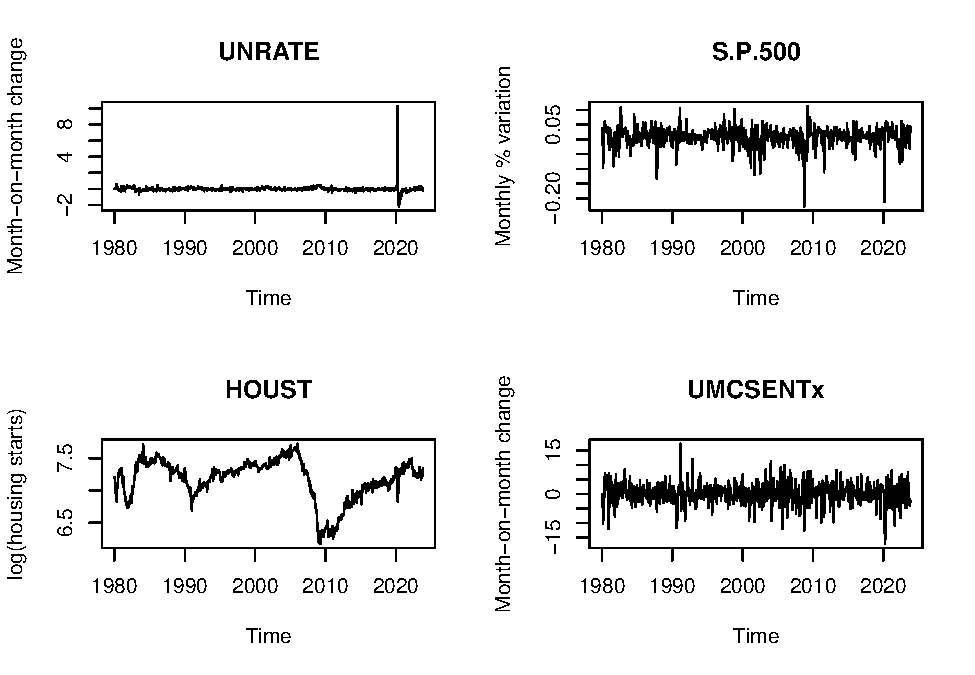
\includegraphics{_main_files/figure-latex/unnamed-chunk-31-1.pdf}

We can have a look to the autocorrelation properties of the series.

\begin{Shaded}
\begin{Highlighting}[]
\DocumentationTok{\#\# ACF plot}
\FunctionTok{par}\NormalTok{(}\AttributeTok{mfrow =} \FunctionTok{c}\NormalTok{(}\DecValTok{2}\NormalTok{,}\DecValTok{2}\NormalTok{))}
\FunctionTok{acf}\NormalTok{(unrate, }\AttributeTok{ylim=}\FunctionTok{c}\NormalTok{(}\SpecialCharTok{{-}}\FloatTok{0.1}\NormalTok{,}\DecValTok{1}\NormalTok{), }\AttributeTok{lwd=}\DecValTok{5}\NormalTok{, }\AttributeTok{xlim=}\FunctionTok{c}\NormalTok{(}\DecValTok{0}\NormalTok{,}\DecValTok{25}\NormalTok{), }\AttributeTok{main=}\StringTok{\textquotesingle{}UNRATE\textquotesingle{}}\NormalTok{)}
\FunctionTok{acf}\NormalTok{(sp500,  }\AttributeTok{ylim=}\FunctionTok{c}\NormalTok{(}\SpecialCharTok{{-}}\FloatTok{0.1}\NormalTok{,}\DecValTok{1}\NormalTok{), }\AttributeTok{lwd=}\DecValTok{5}\NormalTok{, }\AttributeTok{xlim=}\FunctionTok{c}\NormalTok{(}\DecValTok{0}\NormalTok{,}\DecValTok{25}\NormalTok{), }\AttributeTok{main=}\StringTok{\textquotesingle{}S.P.500\textquotesingle{}}\NormalTok{)}
\FunctionTok{acf}\NormalTok{(house,  }\AttributeTok{ylim=}\FunctionTok{c}\NormalTok{(}\SpecialCharTok{{-}}\FloatTok{0.1}\NormalTok{,}\DecValTok{1}\NormalTok{), }\AttributeTok{lwd=}\DecValTok{5}\NormalTok{, }\AttributeTok{xlim=}\FunctionTok{c}\NormalTok{(}\DecValTok{0}\NormalTok{,}\DecValTok{25}\NormalTok{), }\AttributeTok{main=}\StringTok{\textquotesingle{}HOUST\textquotesingle{}}\NormalTok{)}
\FunctionTok{acf}\NormalTok{(sent,   }\AttributeTok{ylim=}\FunctionTok{c}\NormalTok{(}\SpecialCharTok{{-}}\FloatTok{0.1}\NormalTok{,}\DecValTok{1}\NormalTok{), }\AttributeTok{lwd=}\DecValTok{5}\NormalTok{, }\AttributeTok{xlim=}\FunctionTok{c}\NormalTok{(}\DecValTok{0}\NormalTok{,}\DecValTok{25}\NormalTok{), }\AttributeTok{main=}\StringTok{\textquotesingle{}UMCSENTx\textquotesingle{}}\NormalTok{)}
\end{Highlighting}
\end{Shaded}

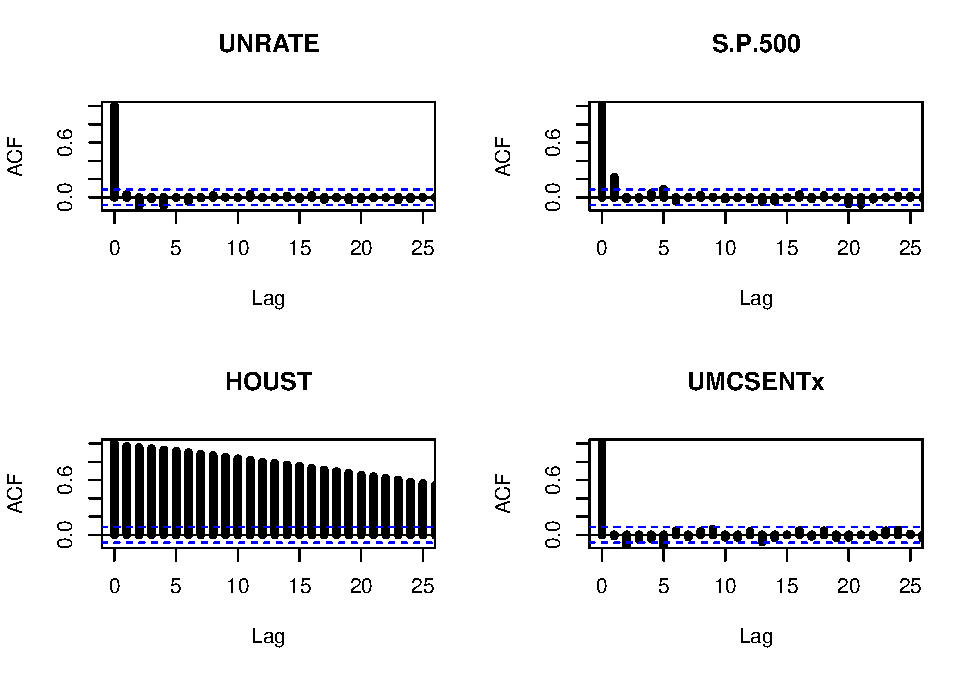
\includegraphics{_main_files/figure-latex/unnamed-chunk-32-1.pdf}

We now study some in-sample properties of the predictive regression:

\[
\begin{aligned}
\text{UNRATE}_t &= \beta_0 + \beta_1 \ \text{UNRATE}_{t-1} + \beta_2 \ \text{HOUST}_{t-1} \ + \beta_3 \ \text{SP500}_{t-1} \ + \beta_4 \ \text{SENT}_{t-1} \ +\\
 &+ \ \text{dummies} \ + \varepsilon_t.
\end{aligned}
\]

In particular, we compute the in-sample predictive fit of the model and we study the properties of the residuals.

\begin{Shaded}
\begin{Highlighting}[]
\DocumentationTok{\#\# Fit predictive regression}
\CommentTok{\# Create the dataframe for regression }
\NormalTok{data\_regression }\OtherTok{\textless{}{-}} \FunctionTok{data.frame}\NormalTok{(}
  \AttributeTok{unrate     =}\NormalTok{ unrate[}\DecValTok{2}\SpecialCharTok{:}\NormalTok{t\_max],}
  \AttributeTok{unrate\_lag =}\NormalTok{ unrate[}\DecValTok{1}\SpecialCharTok{:}\NormalTok{(t\_max}\DecValTok{{-}1}\NormalTok{)],}
  \AttributeTok{house      =}\NormalTok{ house[}\DecValTok{1}\SpecialCharTok{:}\NormalTok{(t\_max}\DecValTok{{-}1}\NormalTok{)],}
  \AttributeTok{sp500      =}\NormalTok{ sp500[}\DecValTok{1}\SpecialCharTok{:}\NormalTok{(t\_max}\DecValTok{{-}1}\NormalTok{)],}
  \AttributeTok{sent       =}\NormalTok{ sent[}\DecValTok{1}\SpecialCharTok{:}\NormalTok{(t\_max}\DecValTok{{-}1}\NormalTok{)],}
  \AttributeTok{d1 =}\NormalTok{ (dates[}\DecValTok{2}\SpecialCharTok{:}\NormalTok{t\_max]}\SpecialCharTok{==}\StringTok{"2020{-}04{-}01"}\NormalTok{)}\SpecialCharTok{*}\DecValTok{1}\NormalTok{, }\CommentTok{\# covid dummy variable}
  \AttributeTok{d2 =}\NormalTok{ (dates[}\DecValTok{2}\SpecialCharTok{:}\NormalTok{t\_max]}\SpecialCharTok{==}\StringTok{"2020{-}05{-}01"}\NormalTok{)}\SpecialCharTok{*}\DecValTok{1}\NormalTok{, }
  \AttributeTok{d3 =}\NormalTok{ (dates[}\DecValTok{2}\SpecialCharTok{:}\NormalTok{t\_max]}\SpecialCharTok{==}\StringTok{"2020{-}06{-}01"}\NormalTok{)}\SpecialCharTok{*}\DecValTok{1}\NormalTok{, }
  \AttributeTok{d4 =}\NormalTok{ (dates[}\DecValTok{2}\SpecialCharTok{:}\NormalTok{t\_max]}\SpecialCharTok{==}\StringTok{"2020{-}07{-}01"}\NormalTok{)}\SpecialCharTok{*}\DecValTok{1}\NormalTok{, }
  \AttributeTok{d5 =}\NormalTok{ (dates[}\DecValTok{2}\SpecialCharTok{:}\NormalTok{t\_max]}\SpecialCharTok{==}\StringTok{"2020{-}08{-}01"}\NormalTok{)}\SpecialCharTok{*}\DecValTok{1}\NormalTok{, }
  \AttributeTok{d6 =}\NormalTok{ (dates[}\DecValTok{2}\SpecialCharTok{:}\NormalTok{t\_max]}\SpecialCharTok{==}\StringTok{"2020{-}09{-}01"}\NormalTok{)}\SpecialCharTok{*}\DecValTok{1} 
\NormalTok{)}

\CommentTok{\# Fit OLS}
\NormalTok{pred\_model }\OtherTok{\textless{}{-}} \FunctionTok{lm}\NormalTok{(unrate }\SpecialCharTok{\textasciitilde{}}\NormalTok{ ., }\AttributeTok{data =}\NormalTok{ data\_regression)}
\NormalTok{vcov\_nw }\OtherTok{\textless{}{-}} \FunctionTok{NeweyWest}\NormalTok{(pred\_model, }\AttributeTok{prewhite=}\NormalTok{F)}

\CommentTok{\# BAD inference (unadjusted asymptotic variance)}
\FunctionTok{coeftest}\NormalTok{(pred\_model)}
\end{Highlighting}
\end{Shaded}

\begin{verbatim}
## 
## t test of coefficients:
## 
##               Estimate Std. Error  t value  Pr(>|t|)    
## (Intercept)  0.6066299  0.1752768   3.4610 0.0005829 ***
## unrate_lag   0.1241838  0.0445711   2.7862 0.0055298 ** 
## house       -0.0854805  0.0244385  -3.4978 0.0005097 ***
## sp500       -0.4989494  0.2318030  -2.1525 0.0318242 *  
## sent        -0.0021749  0.0020826  -1.0443 0.2968167    
## d1          10.0608718  0.1859894  54.0938 < 2.2e-16 ***
## d2          -2.8193347  0.4924891  -5.7247 1.762e-08 ***
## d3          -1.9965983  0.1882808 -10.6044 < 2.2e-16 ***
## d4          -0.4795102  0.2010676  -2.3848 0.0174483 *  
## d5          -1.6764097  0.1795464  -9.3369 < 2.2e-16 ***
## d6          -0.2339512  0.1927566  -1.2137 0.2254137    
## ---
## Signif. codes:  0 '***' 0.001 '**' 0.01 '*' 0.05 '.' 0.1 ' ' 1
\end{verbatim}

\begin{Shaded}
\begin{Highlighting}[]
\CommentTok{\# Inference using the Newey West estimator}
\FunctionTok{coeftest}\NormalTok{(pred\_model, vcov\_nw)}
\end{Highlighting}
\end{Shaded}

\begin{verbatim}
## 
## t test of coefficients:
## 
##               Estimate Std. Error  t value  Pr(>|t|)    
## (Intercept)  0.6066299  0.3400340   1.7840   0.07501 .  
## unrate_lag   0.1241838  0.0686069   1.8101   0.07087 .  
## house       -0.0854805  0.0464922  -1.8386   0.06655 .  
## sp500       -0.4989494  0.2553605  -1.9539   0.05125 .  
## sent        -0.0021749  0.0024861  -0.8748   0.38207    
## d1          10.0608718  0.0970859 103.6286 < 2.2e-16 ***
## d2          -2.8193347  0.7159484  -3.9379 9.351e-05 ***
## d3          -1.9965983  0.1022064 -19.5350 < 2.2e-16 ***
## d4          -0.4795102  0.1528230  -3.1377   0.00180 ** 
## d5          -1.6764097  0.0584554 -28.6785 < 2.2e-16 ***
## d6          -0.2339512  0.1251049  -1.8700   0.06205 .  
## ---
## Signif. codes:  0 '***' 0.001 '**' 0.01 '*' 0.05 '.' 0.1 ' ' 1
\end{verbatim}

\begin{Shaded}
\begin{Highlighting}[]
\CommentTok{\# True VS. predicted values}
\FunctionTok{plot.ts}\NormalTok{(data\_regression}\SpecialCharTok{$}\NormalTok{unrate, }\AttributeTok{ylim =} \FunctionTok{c}\NormalTok{(}\SpecialCharTok{{-}}\FloatTok{0.8}\NormalTok{, }\FloatTok{0.8}\NormalTok{), }\AttributeTok{col =} \StringTok{"darkgrey"}\NormalTok{)}
\FunctionTok{lines}\NormalTok{(}\FunctionTok{predict}\NormalTok{(pred\_model), }\AttributeTok{col =} \StringTok{"darkred"}\NormalTok{)}
\end{Highlighting}
\end{Shaded}

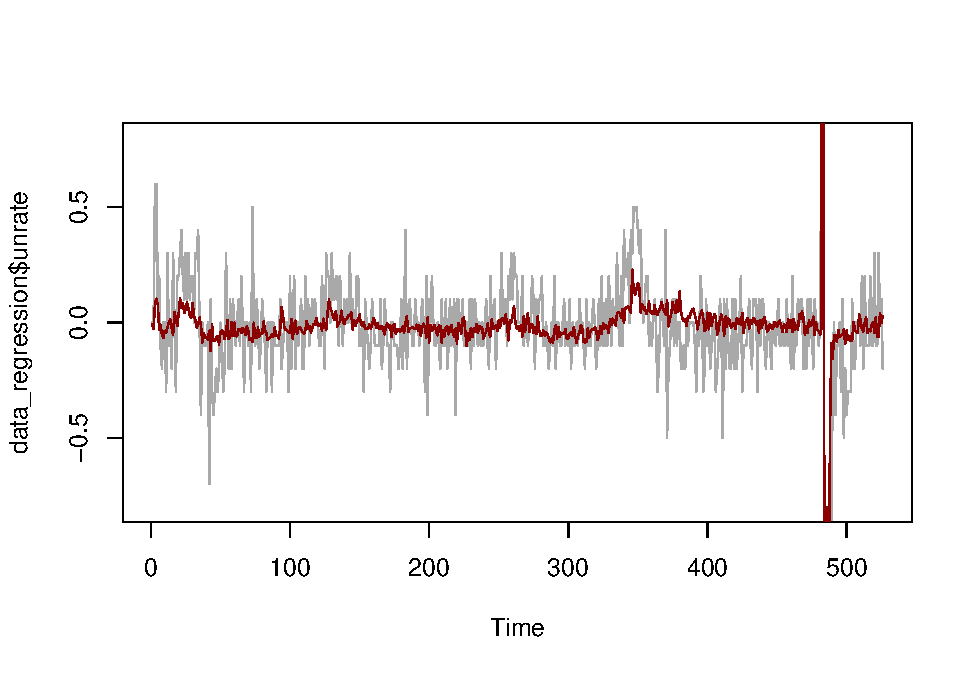
\includegraphics{_main_files/figure-latex/unnamed-chunk-33-1.pdf}

\begin{Shaded}
\begin{Highlighting}[]
\CommentTok{\# Analysis of residuals}
\FunctionTok{acf}\NormalTok{(pred\_model}\SpecialCharTok{$}\NormalTok{residuals, }\AttributeTok{lwd =} \DecValTok{5}\NormalTok{)}
\end{Highlighting}
\end{Shaded}

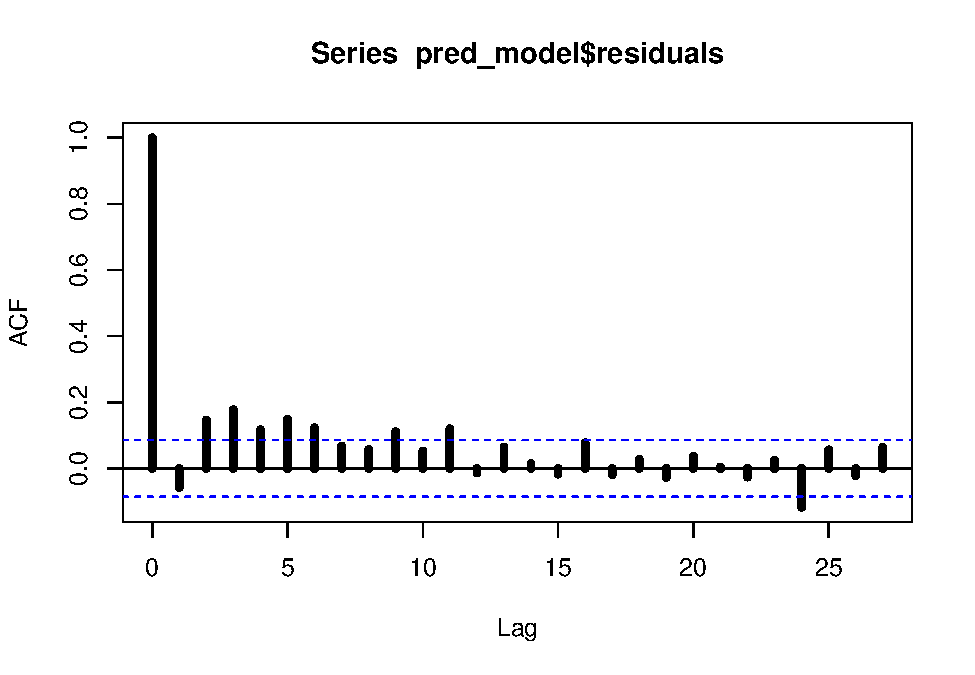
\includegraphics{_main_files/figure-latex/unnamed-chunk-34-1.pdf}

\begin{Shaded}
\begin{Highlighting}[]
\CommentTok{\# Test for autocorrelation}
\FunctionTok{Box.test}\NormalTok{(pred\_model}\SpecialCharTok{$}\NormalTok{residuals, }\AttributeTok{lag=}\DecValTok{12}\NormalTok{)}
\end{Highlighting}
\end{Shaded}

\begin{verbatim}
## 
##  Box-Pierce test
## 
## data:  pred_model$residuals
## X-squared = 76.202, df = 12, p-value = 2.176e-11
\end{verbatim}

We can assess the effect of an exogenous change in the predictors on the target variable over time by using the method of local projections. Here we show the effect of a positive shock in the S.P.500 index.

\begin{Shaded}
\begin{Highlighting}[]
\DocumentationTok{\#\# Local projections for assessing the impact of a shock}
\CommentTok{\# set number of horizons and initialize objects}
\NormalTok{H          }\OtherTok{\textless{}{-}} \DecValTok{12}
\NormalTok{lp         }\OtherTok{\textless{}{-}} \FunctionTok{rep}\NormalTok{(}\DecValTok{0}\NormalTok{,H)      }\CommentTok{\# local projection}
\NormalTok{lp\_confint }\OtherTok{\textless{}{-}} \FunctionTok{matrix}\NormalTok{(}\DecValTok{0}\NormalTok{,H,}\DecValTok{2}\NormalTok{) }\CommentTok{\# confidence intervals}

\CommentTok{\# compute the impact after h = 1,...,H horizons}
\ControlFlowTok{for}\NormalTok{(h }\ControlFlowTok{in} \DecValTok{1}\SpecialCharTok{:}\NormalTok{H)\{}
  \CommentTok{\# prepare dataset for forecasting h periods ahead}
\NormalTok{  data\_h  }\OtherTok{\textless{}{-}} \FunctionTok{cbind}\NormalTok{( }
\NormalTok{    data\_regression[h}\SpecialCharTok{:}\NormalTok{t\_max, }\FunctionTok{c}\NormalTok{(}\StringTok{"unrate"}\NormalTok{, }\FunctionTok{paste0}\NormalTok{(}\StringTok{"d"}\NormalTok{, }\DecValTok{1}\SpecialCharTok{:}\DecValTok{6}\NormalTok{))],}
\NormalTok{    data\_regression[}\DecValTok{1}\SpecialCharTok{:}\NormalTok{(t\_max}\SpecialCharTok{{-}}\NormalTok{h}\SpecialCharTok{+}\DecValTok{1}\NormalTok{), }\FunctionTok{c}\NormalTok{(}\StringTok{"unrate\_lag"}\NormalTok{, }\StringTok{"house"}\NormalTok{, }\StringTok{"sp500"}\NormalTok{, }\StringTok{"sent"}\NormalTok{)]}
\NormalTok{    )}

  \CommentTok{\# predict}
\NormalTok{  pred\_model\_h }\OtherTok{\textless{}{-}} \FunctionTok{lm}\NormalTok{(unrate }\SpecialCharTok{\textasciitilde{}}\NormalTok{ ., }\AttributeTok{data =}\NormalTok{ data\_h)}

  \CommentTok{\# compute Newey{-}West estimate}
\NormalTok{  vcov\_nw\_h }\OtherTok{\textless{}{-}} \FunctionTok{NeweyWest}\NormalTok{(pred\_model\_h, }\AttributeTok{prewhite =}\NormalTok{ F)}

  \CommentTok{\# compute standard errors for the estimated coefficients}
\NormalTok{  confint\_h }\OtherTok{\textless{}{-}} \FunctionTok{coeftest}\NormalTok{(pred\_model\_h, vcov\_nw\_h)}

  \CommentTok{\# store the estimates and the 90\% confidence intervals}
\NormalTok{  lp[h]           }\OtherTok{\textless{}{-}}\NormalTok{ confint\_h[}\StringTok{\textquotesingle{}sp500\textquotesingle{}}\NormalTok{,}\StringTok{\textquotesingle{}Estimate\textquotesingle{}}\NormalTok{]}
\NormalTok{  lp\_confint[h, ] }\OtherTok{\textless{}{-}}\NormalTok{ lp[h] }\SpecialCharTok{+}\NormalTok{ confint\_h[}\StringTok{\textquotesingle{}sp500\textquotesingle{}}\NormalTok{,}\StringTok{\textquotesingle{}Std. Error\textquotesingle{}}\NormalTok{]}\SpecialCharTok{*}\FunctionTok{c}\NormalTok{(}\SpecialCharTok{{-}}\DecValTok{1}\NormalTok{,}\DecValTok{1}\NormalTok{)}\SpecialCharTok{*}\FunctionTok{qnorm}\NormalTok{(}\FloatTok{0.05}\NormalTok{)}
\NormalTok{\}}
\end{Highlighting}
\end{Shaded}

\begin{Shaded}
\begin{Highlighting}[]
\DocumentationTok{\#\# Plot the impulse response function}
\FunctionTok{plot}\NormalTok{(}\DecValTok{1}\SpecialCharTok{:}\NormalTok{H, lp,         }\AttributeTok{lwd =} \DecValTok{3}\NormalTok{, }\AttributeTok{col =} \StringTok{\textquotesingle{}darkred\textquotesingle{}}\NormalTok{, }\AttributeTok{t =} \StringTok{"b"}\NormalTok{, }\AttributeTok{ylim =} \FunctionTok{c}\NormalTok{(}\SpecialCharTok{{-}}\DecValTok{2}\NormalTok{,}\DecValTok{1}\NormalTok{),}
     \AttributeTok{main =} \StringTok{"Response of unemployment after a positive shock on the S.P.500"}\NormalTok{,}
     \AttributeTok{xlab =} \StringTok{""}\NormalTok{, }\AttributeTok{ylab =} \StringTok{""}\NormalTok{)}
\FunctionTok{lines}\NormalTok{(lp\_confint[,}\DecValTok{1}\NormalTok{], }\AttributeTok{lwd =} \DecValTok{1}\NormalTok{, }\AttributeTok{col =} \StringTok{\textquotesingle{}darkred\textquotesingle{}}\NormalTok{, }\AttributeTok{t =} \StringTok{"b"}\NormalTok{, }\AttributeTok{pch  =} \DecValTok{25}\NormalTok{)}
\FunctionTok{lines}\NormalTok{(lp\_confint[,}\DecValTok{2}\NormalTok{], }\AttributeTok{lwd =} \DecValTok{1}\NormalTok{, }\AttributeTok{col =} \StringTok{\textquotesingle{}darkred\textquotesingle{}}\NormalTok{, }\AttributeTok{t =} \StringTok{"b"}\NormalTok{, }\AttributeTok{pch  =} \DecValTok{24}\NormalTok{)}
\FunctionTok{grid}\NormalTok{()}
\FunctionTok{box}\NormalTok{()}
\FunctionTok{abline}\NormalTok{(}\AttributeTok{h=}\DecValTok{0}\NormalTok{,}\AttributeTok{lwd=}\DecValTok{3}\NormalTok{)}
\end{Highlighting}
\end{Shaded}

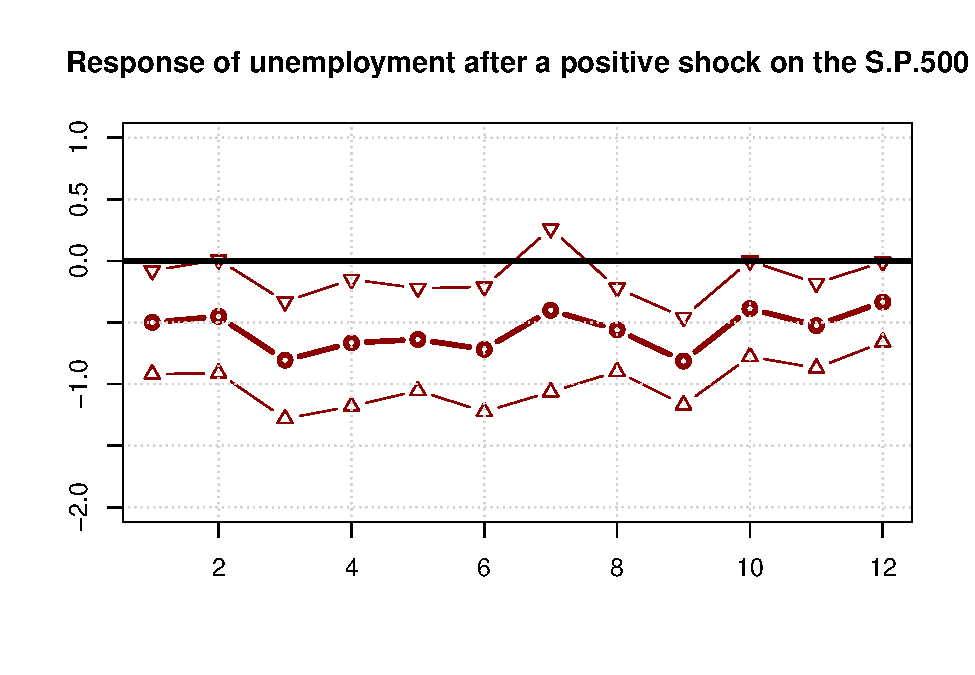
\includegraphics{_main_files/figure-latex/unnamed-chunk-37-1.pdf}

We now proceed to evaluate the forecasts of the model. To do so, we split the data into a training set (observations up to 1999:12) and a testing set (starting in 2000:01). We estimate the parameters of the model on the training data and then make predictions based on the value of the predictors and the estimated coefficients. We compare the forecasts against the sample mean using the MSE. The Diebold-Mariano test suggests that the regression method has a superior forecasting performance than the sample mean. However, this result depends on the specification of the regression model and the predictive ability of the model is still pretty poor.

\begin{Shaded}
\begin{Highlighting}[]
\DocumentationTok{\#\# Forecast evaluation}
\CommentTok{\# split training set (1980{-}2000) and testing set (2000{-}2024)}
\NormalTok{in\_sample  }\OtherTok{\textless{}{-}}\NormalTok{ (dates[}\DecValTok{2}\SpecialCharTok{:}\NormalTok{t\_max] }\SpecialCharTok{\textless{}} \FunctionTok{as.Date}\NormalTok{(}\StringTok{\textquotesingle{}2000{-}01{-}01\textquotesingle{}}\NormalTok{))}
\NormalTok{out\_sample }\OtherTok{\textless{}{-}}\NormalTok{ (dates[}\DecValTok{2}\SpecialCharTok{:}\NormalTok{t\_max] }\SpecialCharTok{\textgreater{}=} \FunctionTok{as.Date}\NormalTok{(}\StringTok{\textquotesingle{}2000{-}01{-}01\textquotesingle{}}\NormalTok{) }\SpecialCharTok{\&} 
\NormalTok{                 ( dates[}\DecValTok{2}\SpecialCharTok{:}\NormalTok{t\_max] }\SpecialCharTok{\textless{}} \FunctionTok{as.Date}\NormalTok{(}\StringTok{\textquotesingle{}2020{-}03{-}01\textquotesingle{}}\NormalTok{) }\SpecialCharTok{|} 
\NormalTok{                     dates[}\DecValTok{2}\SpecialCharTok{:}\NormalTok{t\_max] }\SpecialCharTok{\textgreater{}=} \FunctionTok{as.Date}\NormalTok{(}\StringTok{\textquotesingle{}2020{-}09{-}01\textquotesingle{}}\NormalTok{) ))}
\NormalTok{data\_train }\OtherTok{\textless{}{-}}\NormalTok{ data\_regression[in\_sample,]}
\NormalTok{data\_test }\OtherTok{\textless{}{-}}\NormalTok{ data\_regression[out\_sample,]}
\NormalTok{dates\_test }\OtherTok{\textless{}{-}}\NormalTok{ (dates[}\DecValTok{2}\SpecialCharTok{:}\NormalTok{t\_max])[out\_sample]}

\CommentTok{\# fit predictive models}
\NormalTok{model1 }\OtherTok{\textless{}{-}} \FunctionTok{lm}\NormalTok{(unrate }\SpecialCharTok{\textasciitilde{}}\NormalTok{ unrate\_lag }\SpecialCharTok{+}\NormalTok{ sp500 }\SpecialCharTok{+}\NormalTok{ sent }\SpecialCharTok{+}\NormalTok{ house, }\AttributeTok{data =}\NormalTok{ data\_train)}
\NormalTok{model2 }\OtherTok{\textless{}{-}} \FunctionTok{lm}\NormalTok{(unrate }\SpecialCharTok{\textasciitilde{}}\NormalTok{ unrate\_lag }\SpecialCharTok{+}\NormalTok{ sp500 }\SpecialCharTok{+}\NormalTok{ sent,         }\AttributeTok{data =}\NormalTok{ data\_train)}
\NormalTok{model3 }\OtherTok{\textless{}{-}} \FunctionTok{lm}\NormalTok{(unrate }\SpecialCharTok{\textasciitilde{}}\NormalTok{ unrate\_lag }\SpecialCharTok{+}\NormalTok{ sp500,                }\AttributeTok{data =}\NormalTok{ data\_train)}

\CommentTok{\# get predictions}
\NormalTok{y\_hat1 }\OtherTok{\textless{}{-}} \FunctionTok{predict}\NormalTok{(model1, }\AttributeTok{newdata =}\NormalTok{ data\_test)}
\NormalTok{y\_hat2 }\OtherTok{\textless{}{-}} \FunctionTok{predict}\NormalTok{(model2, }\AttributeTok{newdata =}\NormalTok{ data\_test)}
\NormalTok{y\_hat3 }\OtherTok{\textless{}{-}} \FunctionTok{predict}\NormalTok{(model3, }\AttributeTok{newdata =}\NormalTok{ data\_test)}

\CommentTok{\# compute benchmark prediction (sample mean)}
\NormalTok{y\_benchmark  }\OtherTok{\textless{}{-}} \FunctionTok{rep}\NormalTok{(}\FunctionTok{mean}\NormalTok{(data\_train}\SpecialCharTok{$}\NormalTok{unrate), }\FunctionTok{sum}\NormalTok{(out\_sample))}

\CommentTok{\# compute MSE}
\NormalTok{mse\_model1     }\OtherTok{\textless{}{-}} \FunctionTok{mse}\NormalTok{(data\_test}\SpecialCharTok{$}\NormalTok{unrate, y\_hat1)}
\NormalTok{mse\_model2     }\OtherTok{\textless{}{-}} \FunctionTok{mse}\NormalTok{(data\_test}\SpecialCharTok{$}\NormalTok{unrate, y\_hat2)}
\NormalTok{mse\_model3     }\OtherTok{\textless{}{-}} \FunctionTok{mse}\NormalTok{(data\_test}\SpecialCharTok{$}\NormalTok{unrate, y\_hat3)}
\NormalTok{mse\_benchmark  }\OtherTok{\textless{}{-}} \FunctionTok{mse}\NormalTok{(data\_test}\SpecialCharTok{$}\NormalTok{unrate, y\_benchmark)}

\CommentTok{\# results}
\FunctionTok{round}\NormalTok{(}\FunctionTok{rbind}\NormalTok{(}
  \AttributeTok{mse\_4vars =}\NormalTok{ mse\_model1,}
  \AttributeTok{mse\_3vars =}\NormalTok{ mse\_model2,}
  \AttributeTok{mse\_2vars =}\NormalTok{ mse\_model3,}
  \AttributeTok{mse\_mean  =}\NormalTok{ mse\_benchmark,}
  \AttributeTok{R2\_2vars  =} \DecValTok{1} \SpecialCharTok{{-}}\NormalTok{ mse\_model3}\SpecialCharTok{/}\NormalTok{mse\_benchmark        }
\NormalTok{), }\DecValTok{4}\NormalTok{)}
\end{Highlighting}
\end{Shaded}

\begin{verbatim}
##             [,1]
## mse_4vars 0.0536
## mse_3vars 0.0302
## mse_2vars 0.0296
## mse_mean  0.0318
## R2_2vars  0.0677
\end{verbatim}

\begin{Shaded}
\begin{Highlighting}[]
\CommentTok{\# convert to ts object to have dates in plot}
\NormalTok{y\_true }\OtherTok{\textless{}{-}} \FunctionTok{ts}\NormalTok{(data\_test}\SpecialCharTok{$}\NormalTok{unrate, }\AttributeTok{start =} \FunctionTok{c}\NormalTok{(}\DecValTok{2000}\NormalTok{, }\DecValTok{1}\NormalTok{), }\AttributeTok{frequency =} \DecValTok{12}\NormalTok{)}
\NormalTok{y\_hat3 }\OtherTok{\textless{}{-}} \FunctionTok{ts}\NormalTok{(y\_hat3, }\AttributeTok{start =} \FunctionTok{c}\NormalTok{(}\DecValTok{2000}\NormalTok{, }\DecValTok{1}\NormalTok{), }\AttributeTok{frequency =} \DecValTok{12}\NormalTok{)}
\NormalTok{y\_benchmark }\OtherTok{\textless{}{-}} \FunctionTok{ts}\NormalTok{(y\_benchmark, }\AttributeTok{start =} \FunctionTok{c}\NormalTok{(}\DecValTok{2000}\NormalTok{, }\DecValTok{1}\NormalTok{), }\AttributeTok{frequency =} \DecValTok{12}\NormalTok{)}

\CommentTok{\# plot}
\FunctionTok{plot.ts}\NormalTok{(y\_true, }\AttributeTok{col =} \StringTok{"darkgrey"}\NormalTok{, }\AttributeTok{ylim =} \FunctionTok{c}\NormalTok{(}\SpecialCharTok{{-}}\FloatTok{0.4}\NormalTok{, }\FloatTok{0.2}\NormalTok{), }
        \AttributeTok{main =} \StringTok{"Forecasted values of unemployment change"}\NormalTok{,}
        \AttributeTok{ylab =} \StringTok{"Change in unemployment rate"}\NormalTok{, }
        \AttributeTok{xlab =} \StringTok{""}\NormalTok{)}
\FunctionTok{lines}\NormalTok{(y\_hat3, }\AttributeTok{col =} \StringTok{"darkred"}\NormalTok{, }\AttributeTok{lwd =} \DecValTok{2}\NormalTok{)}
\FunctionTok{lines}\NormalTok{(y\_benchmark)}
\FunctionTok{rect}\NormalTok{(}\FloatTok{2020.25}\NormalTok{,}\SpecialCharTok{{-}}\DecValTok{1}\NormalTok{,}\FloatTok{2020.75}\NormalTok{,}\DecValTok{1}\NormalTok{,}\AttributeTok{col =} \FunctionTok{rgb}\NormalTok{(}\FloatTok{0.6}\NormalTok{,}\FloatTok{0.1}\NormalTok{,}\FloatTok{0.1}\NormalTok{,}\DecValTok{1}\SpecialCharTok{/}\DecValTok{4}\NormalTok{))}
\FunctionTok{legend}\NormalTok{(}\StringTok{"bottomleft"}\NormalTok{, }\FunctionTok{c}\NormalTok{(}\StringTok{"Forecast"}\NormalTok{, }\StringTok{"True"}\NormalTok{), }\AttributeTok{col=}\FunctionTok{c}\NormalTok{(}\StringTok{"darkred"}\NormalTok{, }\StringTok{"darkgrey"}\NormalTok{), }\AttributeTok{lwd=}\DecValTok{6}\NormalTok{)}
\end{Highlighting}
\end{Shaded}

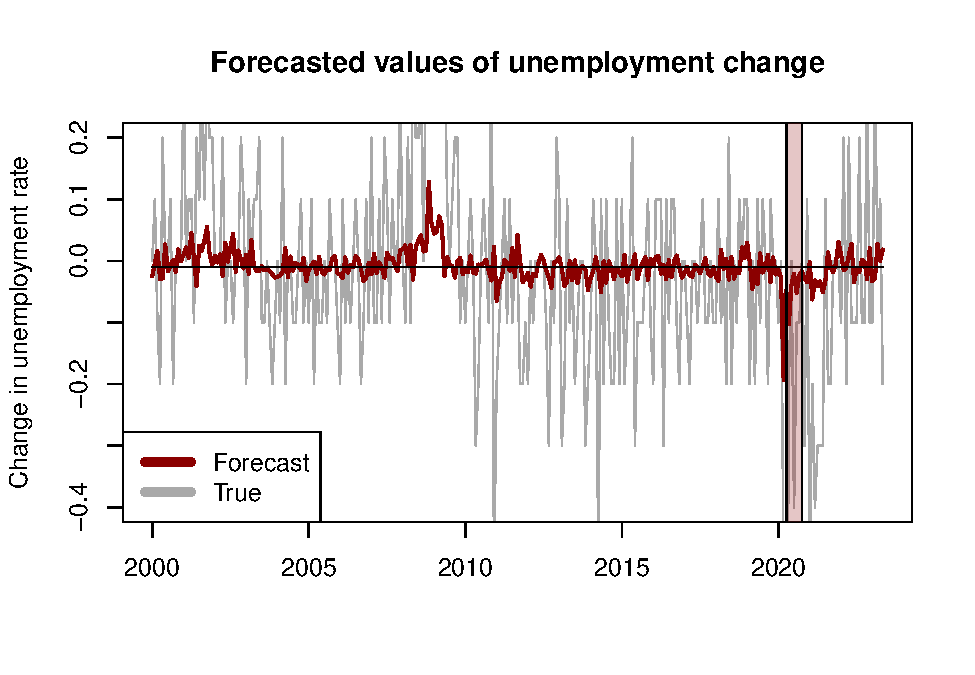
\includegraphics{_main_files/figure-latex/unnamed-chunk-39-1.pdf}

It is common to report the plot of the normalized cumulated squared errors to assess if one model has a superior forecasting ability over all the testing period:

\[
\text{Cumulated error}_t =  \frac{\sum_{\tau = t_w + 1}^t e_\tau^2}{\sum_{\tau = t_w + 1}^T \bar{e}_{\tau}^2}
\]

where \(e_\tau, \bar{e}_\tau\) denote respectively the forecast error of the model and the benchmark at time \(\tau\), and \(t_w\) is the number of periods in the training set.

\begin{Shaded}
\begin{Highlighting}[]
\DocumentationTok{\#\# Plot the forecast errors over time}
\CommentTok{\# compute the forecast errors}
\NormalTok{err\_model }\OtherTok{\textless{}{-}}\NormalTok{ y\_true}\SpecialCharTok{{-}}\NormalTok{y\_hat3}
\NormalTok{err\_benchmark }\OtherTok{\textless{}{-}}\NormalTok{ y\_true}\SpecialCharTok{{-}}\NormalTok{y\_benchmark}
\CommentTok{\# compute the (normalized) cumulated squared errors and convert to ts object}
\NormalTok{err2\_model     }\OtherTok{\textless{}{-}} \FunctionTok{ts}\NormalTok{(}\FunctionTok{cumsum}\NormalTok{((err\_model)}\SpecialCharTok{\^{}}\DecValTok{2}\NormalTok{), }\AttributeTok{start =} \FunctionTok{c}\NormalTok{(}\DecValTok{2000}\NormalTok{, }\DecValTok{1}\NormalTok{), }\AttributeTok{frequency =} \DecValTok{12}\NormalTok{)}
\NormalTok{err2\_benchmark }\OtherTok{\textless{}{-}} \FunctionTok{ts}\NormalTok{(}\FunctionTok{cumsum}\NormalTok{((err\_benchmark)}\SpecialCharTok{\^{}}\DecValTok{2}\NormalTok{), }\AttributeTok{start =} \FunctionTok{c}\NormalTok{(}\DecValTok{2000}\NormalTok{, }\DecValTok{1}\NormalTok{), }\AttributeTok{frequency =} \DecValTok{12}\NormalTok{)}
\NormalTok{err2\_constant  }\OtherTok{\textless{}{-}} \FunctionTok{sum}\NormalTok{((y\_true}\SpecialCharTok{{-}}\NormalTok{y\_benchmark)}\SpecialCharTok{\^{}}\DecValTok{2}\NormalTok{)}
\CommentTok{\# plot the cumulated squared errors over time}
\FunctionTok{plot.ts}\NormalTok{(err2\_benchmark}\SpecialCharTok{/}\NormalTok{err2\_constant, }\AttributeTok{lwd =} \DecValTok{2}\NormalTok{,}
        \AttributeTok{ylab =} \StringTok{"Cumulated squared errors"}\NormalTok{,}
        \AttributeTok{main =} \StringTok{"Forecast errors over time"}\NormalTok{,}
        \AttributeTok{xlab =} \StringTok{""}\NormalTok{)}
\FunctionTok{lines}\NormalTok{(err2\_model}\SpecialCharTok{/}\NormalTok{err2\_constant, }\AttributeTok{col =} \StringTok{"darkred"}\NormalTok{, }\AttributeTok{lwd =} \DecValTok{2}\NormalTok{)}
\FunctionTok{rect}\NormalTok{(}\FloatTok{2020.25}\NormalTok{,}\SpecialCharTok{{-}}\DecValTok{1}\NormalTok{,}\FloatTok{2020.75}\NormalTok{,}\FloatTok{1.5}\NormalTok{,}\AttributeTok{col =} \FunctionTok{rgb}\NormalTok{(}\FloatTok{0.6}\NormalTok{,}\FloatTok{0.1}\NormalTok{,}\FloatTok{0.1}\NormalTok{,}\DecValTok{1}\SpecialCharTok{/}\DecValTok{4}\NormalTok{))}
\FunctionTok{legend}\NormalTok{(}\StringTok{"topleft"}\NormalTok{, }\FunctionTok{c}\NormalTok{(}\StringTok{"Regression model"}\NormalTok{, }\StringTok{"Sample mean"}\NormalTok{), }\AttributeTok{col=}\FunctionTok{c}\NormalTok{(}\StringTok{"darkred"}\NormalTok{, }\StringTok{"black"}\NormalTok{), }\AttributeTok{lwd=}\DecValTok{6}\NormalTok{)}
\end{Highlighting}
\end{Shaded}

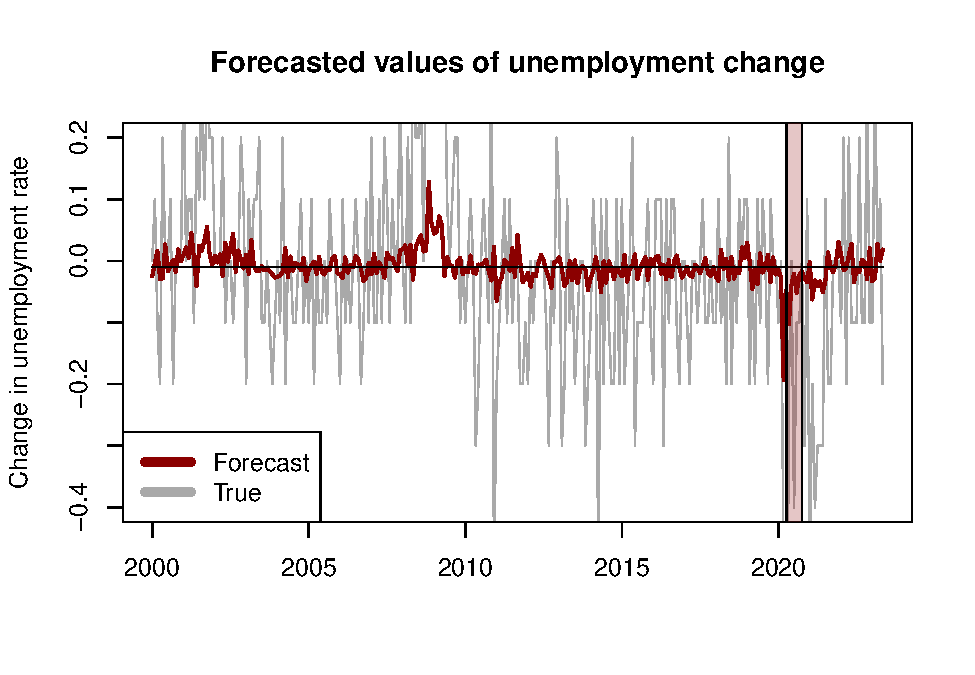
\includegraphics{_main_files/figure-latex/unnamed-chunk-40-1.pdf}

\begin{Shaded}
\begin{Highlighting}[]
\DocumentationTok{\#\# Diebold{-}Mariano test for predictive performance}
\CommentTok{\# one{-}sided test: }
\CommentTok{\# {-} H0: err\_benchmark = err\_model}
\CommentTok{\# {-} H1: err\_benchmark \textgreater{} err\_model}
\FunctionTok{dm.test}\NormalTok{(err\_benchmark, err\_model, }\AttributeTok{alternative =} \StringTok{"greater"}\NormalTok{) }
\end{Highlighting}
\end{Shaded}

\begin{verbatim}
## 
##  Diebold-Mariano Test
## 
## data:  err_benchmarkerr_model
## DM = 2.4995, Forecast horizon = 1, Loss function power = 2, p-value =
## 0.006504
## alternative hypothesis: greater
\end{verbatim}

\hypertarget{session03}{%
\chapter{Large-dimensional methods for forecasting}\label{session03}}

In this session we compare the performances of four forecasting methods to predict the monthly change in the U.S. unemployment rate using more than 100 variables from the FRED-MD dataset. In order to deal with the large amount of data, we consider methods based on principal component analysis, penalized likelihood and regression trees.

\hypertarget{preprocess-fred-md}{%
\section{Preprocess FRED-MD}\label{preprocess-fred-md}}

The preprocessing of the data is very similar to that of the previous session. The only difference is that we now transform all the series in the dataset using the list of transformation functions of the previous session.

For simplicity, here we remove the columns with missing values. An alternative could be to impute the missing values using some regression technique. However, it is important to notice that in the latter case we should impute the missing values at each step of the forecast evaluation to make sure that no future information is included in the forecasts.

\begin{Shaded}
\begin{Highlighting}[]
\DocumentationTok{\#\# load data}
\NormalTok{fredmd }\OtherTok{\textless{}{-}} \FunctionTok{read.csv}\NormalTok{(}\StringTok{"../data/current.csv"}\NormalTok{)}
\NormalTok{dates  }\OtherTok{\textless{}{-}} \FunctionTok{as.Date}\NormalTok{(fredmd}\SpecialCharTok{$}\NormalTok{sasdate[}\SpecialCharTok{{-}}\DecValTok{1}\NormalTok{],}\StringTok{\textquotesingle{}\%m/\%d/\%Y\textquotesingle{}}\NormalTok{)}
\NormalTok{target\_variables }\OtherTok{\textless{}{-}} \FunctionTok{c}\NormalTok{(}\StringTok{"UNRATE"}\NormalTok{, }\StringTok{"W875RX1"}\NormalTok{, }\StringTok{"GS10"}\NormalTok{, }\StringTok{"CPIAUCSL"}\NormalTok{, }\StringTok{"WPSFD49207"}\NormalTok{, }
                      \StringTok{"PAYEMS"}\NormalTok{, }\StringTok{"HOUST"}\NormalTok{, }\StringTok{"INDPRO"}\NormalTok{, }\StringTok{"M2SL"}\NormalTok{, }\StringTok{"S.P.500"}\NormalTok{)}

\DocumentationTok{\#\# get tcodes}
\NormalTok{tcodes }\OtherTok{\textless{}{-}}\NormalTok{ fredmd[}\DecValTok{1}\NormalTok{,}\SpecialCharTok{{-}}\DecValTok{1}\NormalTok{]}
\NormalTok{d      }\OtherTok{\textless{}{-}}\NormalTok{ fredmd[}\SpecialCharTok{{-}}\DecValTok{1}\NormalTok{, }\SpecialCharTok{{-}}\DecValTok{1}\NormalTok{]}
\end{Highlighting}
\end{Shaded}

\begin{Shaded}
\begin{Highlighting}[]
\DocumentationTok{\#\# Transform variables}
\CommentTok{\# transformation functions}
\NormalTok{transform\_fredmd }\OtherTok{\textless{}{-}} \FunctionTok{list}\NormalTok{(}
  \ControlFlowTok{function}\NormalTok{(x) x,}
  \ControlFlowTok{function}\NormalTok{(x) }\FunctionTok{c}\NormalTok{(}\DecValTok{0}\NormalTok{, }\FunctionTok{diff}\NormalTok{(x)),}
  \ControlFlowTok{function}\NormalTok{(x) }\FunctionTok{c}\NormalTok{(}\DecValTok{0}\NormalTok{, }\DecValTok{0}\NormalTok{, }\FunctionTok{diff}\NormalTok{(x, }\AttributeTok{differences =} \DecValTok{2}\NormalTok{)),}
  \ControlFlowTok{function}\NormalTok{(x) }\FunctionTok{log}\NormalTok{(x),}
  \ControlFlowTok{function}\NormalTok{(x) }\FunctionTok{c}\NormalTok{(}\DecValTok{0}\NormalTok{, }\FunctionTok{diff}\NormalTok{(}\FunctionTok{log}\NormalTok{(x))),}
  \ControlFlowTok{function}\NormalTok{(x) }\FunctionTok{c}\NormalTok{(}\DecValTok{0}\NormalTok{, }\DecValTok{0}\NormalTok{, }\FunctionTok{diff}\NormalTok{(}\FunctionTok{log}\NormalTok{(x), }\AttributeTok{differences =} \DecValTok{2}\NormalTok{)),}
  \ControlFlowTok{function}\NormalTok{(x) }\FunctionTok{c}\NormalTok{(}\DecValTok{0}\NormalTok{, }\DecValTok{0}\NormalTok{, }\FunctionTok{diff}\NormalTok{( x[}\DecValTok{2}\SpecialCharTok{:}\FunctionTok{length}\NormalTok{(x)]}\SpecialCharTok{/}\NormalTok{x[}\DecValTok{1}\SpecialCharTok{:}\NormalTok{(}\FunctionTok{length}\NormalTok{(x)}\SpecialCharTok{{-}}\DecValTok{1}\NormalTok{)] }\SpecialCharTok{{-}} \DecValTok{1}\NormalTok{))}
\NormalTok{)}

\CommentTok{\# transform series one by one}
\ControlFlowTok{for}\NormalTok{ (j }\ControlFlowTok{in} \DecValTok{1}\SpecialCharTok{:}\FunctionTok{ncol}\NormalTok{(d)) \{}
\NormalTok{  tcode }\OtherTok{\textless{}{-}}\NormalTok{ tcodes[[j]]}
\NormalTok{  d[,j] }\OtherTok{\textless{}{-}}\NormalTok{ transform\_fredmd[[tcode]](d[,j])}
\NormalTok{\}}

\DocumentationTok{\#\# Subset and remove columns with NAs}
\NormalTok{d }\OtherTok{\textless{}{-}}\NormalTok{ d[dates }\SpecialCharTok{\textgreater{}=} \StringTok{\textquotesingle{}1980{-}01{-}01\textquotesingle{}}\NormalTok{, ]}
\NormalTok{dates }\OtherTok{\textless{}{-}}\NormalTok{ dates[dates }\SpecialCharTok{\textgreater{}=} \StringTok{\textquotesingle{}1980{-}01{-}01\textquotesingle{}}\NormalTok{]}
\NormalTok{idx\_na }\OtherTok{\textless{}{-}}\NormalTok{ (}\FunctionTok{colSums}\NormalTok{(}\FunctionTok{is.na}\NormalTok{(d))}\SpecialCharTok{==}\DecValTok{0}\NormalTok{)}
\NormalTok{d }\OtherTok{\textless{}{-}}\NormalTok{ d[, idx\_na]}
\FunctionTok{plot.ts}\NormalTok{(d[,target\_variables])}
\end{Highlighting}
\end{Shaded}

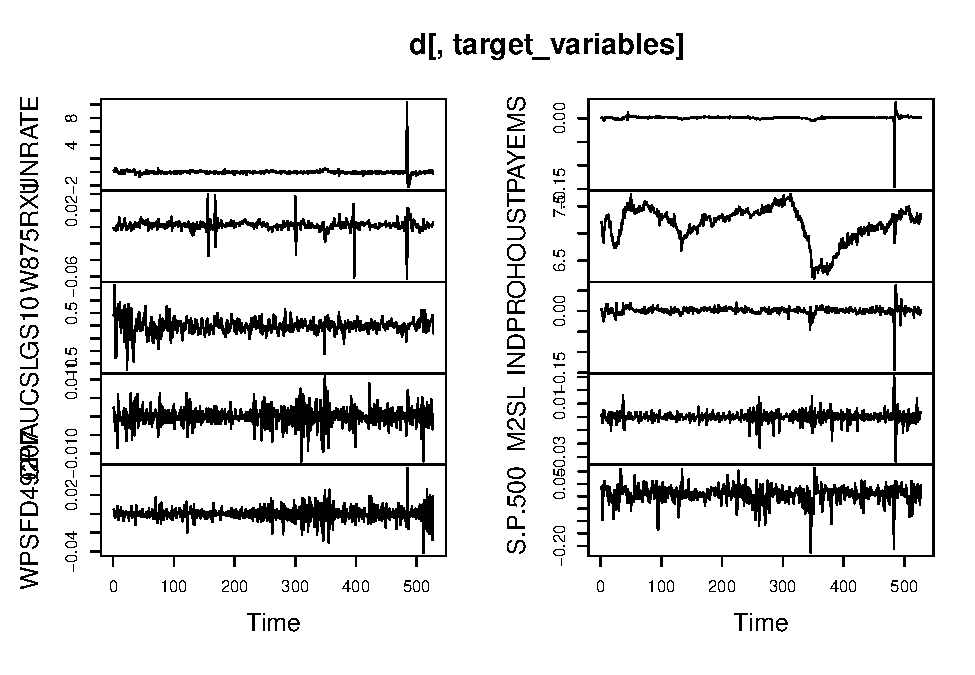
\includegraphics{_main_files/figure-latex/unnamed-chunk-43-1.pdf}

\hypertarget{forecasting-algorithms}{%
\section{Forecasting algorithms}\label{forecasting-algorithms}}

Below we define the forecasting algorithms that we use in the forecast evaluation.

Notice that at each step of the forecast evaluation we rescale the data so that each variable has mean zero and unit variance. This step is very important for many machine learning algorithms. If the variables have a different magnitude, the optimization procedure involved tend to over-focus on the features with higher magnitude, while we want to exploit the variability of each feature irrespectively of its scale.

Also, we do not explicitly account for outliers in the forecasting algorithms, and we simply discard the Covid period during the evaluation of the results. In this sense, the procedure will tend to benefit those methods that can automatically deal better with the presence of outliers in the data used for estimation.

\begin{Shaded}
\begin{Highlighting}[]
\DocumentationTok{\#\# Principal Component Regression (PCR)}
\NormalTok{pcr }\OtherTok{\textless{}{-}} \ControlFlowTok{function}\NormalTok{(d, target, n\_components, horizon) \{}
  
  \DocumentationTok{\#\# Scale the data}
\NormalTok{  d\_scaled }\OtherTok{\textless{}{-}} \FunctionTok{scale}\NormalTok{(d)}
\NormalTok{  d\_mean }\OtherTok{\textless{}{-}} \FunctionTok{attr}\NormalTok{(d\_scaled, }\StringTok{"scaled:center"}\NormalTok{)}
\NormalTok{  d\_sd }\OtherTok{\textless{}{-}} \FunctionTok{attr}\NormalTok{(d\_scaled, }\StringTok{"scaled:scale"}\NormalTok{)}
  
  \DocumentationTok{\#\# get the target}
\NormalTok{  target\_idx }\OtherTok{\textless{}{-}} \FunctionTok{which}\NormalTok{(}\FunctionTok{colnames}\NormalTok{(d) }\SpecialCharTok{==}\NormalTok{ target)}
\NormalTok{  y }\OtherTok{\textless{}{-}}\NormalTok{ d\_scaled[,target\_idx]    }
  \DocumentationTok{\#\# get the principal components of the other variables}
\NormalTok{  x }\OtherTok{\textless{}{-}}\NormalTok{ d\_scaled[,}\SpecialCharTok{{-}}\NormalTok{target\_idx]}
\NormalTok{  eigen\_list }\OtherTok{\textless{}{-}} \FunctionTok{prcomp}\NormalTok{(x, }\AttributeTok{center=}\ConstantTok{FALSE}\NormalTok{)}
\NormalTok{  f }\OtherTok{\textless{}{-}}\NormalTok{ eigen\_list}\SpecialCharTok{$}\NormalTok{x[,}\DecValTok{1}\SpecialCharTok{:}\NormalTok{n\_components] }
  
  \DocumentationTok{\#\# define the dataframes }
\NormalTok{  t\_max }\OtherTok{\textless{}{-}} \FunctionTok{length}\NormalTok{(y)}
\NormalTok{  d\_pcr }\OtherTok{\textless{}{-}} \FunctionTok{as.data.frame}\NormalTok{(}\FunctionTok{cbind}\NormalTok{(}
    \AttributeTok{y     =}\NormalTok{ y[(horizon}\SpecialCharTok{+}\DecValTok{1}\NormalTok{)}\SpecialCharTok{:}\NormalTok{t\_max], }
    \AttributeTok{y\_lag =}\NormalTok{  y[}\DecValTok{1}\SpecialCharTok{:}\NormalTok{(t\_max}\SpecialCharTok{{-}}\NormalTok{horizon)],  }
\NormalTok{    f[}\DecValTok{1}\SpecialCharTok{:}\NormalTok{(t\_max}\SpecialCharTok{{-}}\NormalTok{horizon),])}
\NormalTok{  )}
  
  \DocumentationTok{\#\# fit}
\NormalTok{  model }\OtherTok{\textless{}{-}} \FunctionTok{lm}\NormalTok{(y }\SpecialCharTok{\textasciitilde{}}\NormalTok{ ., }\AttributeTok{data =}\NormalTok{ d\_pcr)}
  
  \DocumentationTok{\#\# forecast}
\NormalTok{  pred }\OtherTok{\textless{}{-}} \FunctionTok{predict}\NormalTok{(model, }\AttributeTok{newdata =}\NormalTok{ d\_pcr[}\FunctionTok{nrow}\NormalTok{(d\_pcr), ])}
  
  \DocumentationTok{\#\# output}
\NormalTok{  pred}\SpecialCharTok{*}\NormalTok{d\_sd[target] }\SpecialCharTok{+}\NormalTok{ d\_mean[target]}
\NormalTok{\}}

\CommentTok{\# pcr(d, "INDPRO", 4, 1)}
\end{Highlighting}
\end{Shaded}

\begin{Shaded}
\begin{Highlighting}[]
\DocumentationTok{\#\# Penalized regression: LASSO (alpha = 1) and ridge (alpha = 0)}
\FunctionTok{library}\NormalTok{(glmnet)}
\end{Highlighting}
\end{Shaded}

\begin{verbatim}
## Caricamento del pacchetto richiesto: Matrix
\end{verbatim}

\begin{verbatim}
## Loaded glmnet 4.1-4
\end{verbatim}

\begin{Shaded}
\begin{Highlighting}[]
\NormalTok{penalized\_reg }\OtherTok{\textless{}{-}} \ControlFlowTok{function}\NormalTok{(d, target, horizon, }\AttributeTok{alpha =} \DecValTok{1}\NormalTok{, }\AttributeTok{nlambda =} \DecValTok{100}\NormalTok{) \{}
  
  \DocumentationTok{\#\# Scale the data}
\NormalTok{  d\_scaled }\OtherTok{\textless{}{-}} \FunctionTok{scale}\NormalTok{(d)}
\NormalTok{  d\_mean }\OtherTok{\textless{}{-}} \FunctionTok{attr}\NormalTok{(d\_scaled, }\StringTok{"scaled:center"}\NormalTok{)}
\NormalTok{  d\_sd }\OtherTok{\textless{}{-}} \FunctionTok{attr}\NormalTok{(d\_scaled, }\StringTok{"scaled:scale"}\NormalTok{)}
  
  \DocumentationTok{\#\# get the target and predictors}
\NormalTok{  t\_max }\OtherTok{\textless{}{-}} \FunctionTok{nrow}\NormalTok{(d)}
\NormalTok{  y }\OtherTok{\textless{}{-}}\NormalTok{ d\_scaled[(horizon}\SpecialCharTok{+}\DecValTok{1}\NormalTok{)}\SpecialCharTok{:}\NormalTok{t\_max, target]   }
\NormalTok{  x }\OtherTok{\textless{}{-}}\NormalTok{ d\_scaled[}\DecValTok{1}\SpecialCharTok{:}\NormalTok{(t\_max}\SpecialCharTok{{-}}\NormalTok{horizon), ] }\CommentTok{\# include also lagged target variable}
  
  \DocumentationTok{\#\# fit the model}
\NormalTok{  model }\OtherTok{\textless{}{-}} \FunctionTok{glmnet}\NormalTok{(}\AttributeTok{x =}\NormalTok{ x, }\AttributeTok{y =}\NormalTok{ y, }\AttributeTok{family =} \StringTok{"gaussian"}\NormalTok{, }
                  \AttributeTok{alpha =}\NormalTok{ alpha, }\AttributeTok{nlambda =}\NormalTok{ nlambda)}
  
  \DocumentationTok{\#\# forecast}
\NormalTok{  pred }\OtherTok{\textless{}{-}} \FunctionTok{predict}\NormalTok{(model, }\AttributeTok{newx =}\NormalTok{ x[}\FunctionTok{nrow}\NormalTok{(x),])}
  
  \DocumentationTok{\#\# Output}
\NormalTok{  pred}\SpecialCharTok{*}\NormalTok{d\_sd[target] }\SpecialCharTok{+}\NormalTok{ d\_mean[target]}
\NormalTok{\}}

\CommentTok{\# penalized\_reg(d, "INDPRO", 1, 1) \# one value for each lambda}
\end{Highlighting}
\end{Shaded}

\begin{Shaded}
\begin{Highlighting}[]
\DocumentationTok{\#\# Random forest}
\FunctionTok{library}\NormalTok{(randomForest)}
\NormalTok{forest }\OtherTok{\textless{}{-}} \ControlFlowTok{function}\NormalTok{(d, target, horizon, }\AttributeTok{seed =} \DecValTok{1}\NormalTok{, }\AttributeTok{ntree =} \DecValTok{100}\NormalTok{) \{}
  
  \DocumentationTok{\#\# Scale the data}
\NormalTok{  d\_scaled }\OtherTok{\textless{}{-}} \FunctionTok{scale}\NormalTok{(d)}
\NormalTok{  d\_mean }\OtherTok{\textless{}{-}} \FunctionTok{attr}\NormalTok{(d\_scaled, }\StringTok{"scaled:center"}\NormalTok{)}
\NormalTok{  d\_sd }\OtherTok{\textless{}{-}} \FunctionTok{attr}\NormalTok{(d\_scaled, }\StringTok{"scaled:scale"}\NormalTok{)}
  
  \DocumentationTok{\#\# get the target and predictors}
\NormalTok{  t\_max }\OtherTok{\textless{}{-}} \FunctionTok{nrow}\NormalTok{(d)}
\NormalTok{  y }\OtherTok{\textless{}{-}}\NormalTok{ d\_scaled[(horizon}\SpecialCharTok{+}\DecValTok{1}\NormalTok{)}\SpecialCharTok{:}\NormalTok{t\_max, target]   }
\NormalTok{  x }\OtherTok{\textless{}{-}}\NormalTok{ d\_scaled[}\DecValTok{1}\SpecialCharTok{:}\NormalTok{(t\_max}\SpecialCharTok{{-}}\NormalTok{horizon), ] }\CommentTok{\# include also lagged target variable}
  
  \DocumentationTok{\#\# fit the model}
  \FunctionTok{set.seed}\NormalTok{(seed)}
\NormalTok{  model }\OtherTok{\textless{}{-}} \FunctionTok{randomForest}\NormalTok{(}\AttributeTok{x =}\NormalTok{ x, }\AttributeTok{y =}\NormalTok{ y, }\AttributeTok{ntree =}\NormalTok{ ntree)}
  
  \DocumentationTok{\#\# forecast}
\NormalTok{  pred }\OtherTok{\textless{}{-}} \FunctionTok{predict}\NormalTok{(model, }\AttributeTok{newdata =}\NormalTok{ x[}\FunctionTok{nrow}\NormalTok{(x),])}

  \DocumentationTok{\#\# Output}
\NormalTok{  pred}\SpecialCharTok{*}\NormalTok{d\_sd[target] }\SpecialCharTok{+}\NormalTok{ d\_mean[target]}
\NormalTok{\}}

\CommentTok{\# forest(d, "INDPRO", 1)}
\end{Highlighting}
\end{Shaded}

\hypertarget{forecast-evaluation}{%
\section{Forecast evaluation}\label{forecast-evaluation}}

We can now run the algorithms and compare their forecasting performances over the 2002-2020 period.

\begin{Shaded}
\begin{Highlighting}[]
\DocumentationTok{\#\# Initialize objects}
\NormalTok{forecast\_list }\OtherTok{\textless{}{-}} \FunctionTok{list}\NormalTok{(}
  \AttributeTok{pcr =} \FunctionTok{c}\NormalTok{(),}
  \AttributeTok{ridge =} \FunctionTok{list}\NormalTok{(),}
  \AttributeTok{lasso =} \FunctionTok{list}\NormalTok{(),}
  \AttributeTok{forest =} \FunctionTok{c}\NormalTok{()}
\NormalTok{)}
\CommentTok{\# choose target variable and forecast horizon}
\NormalTok{target }\OtherTok{\textless{}{-}} \StringTok{"UNRATE"}
\NormalTok{horizon }\OtherTok{\textless{}{-}} \DecValTok{1}

\CommentTok{\# pick the initial window for training and choose the test period}
\NormalTok{initial\_window }\OtherTok{\textless{}{-}} \FunctionTok{sum}\NormalTok{(dates }\SpecialCharTok{\textless{}} \StringTok{"2002{-}01{-}01"}\NormalTok{)}
\NormalTok{idx\_eval }\OtherTok{\textless{}{-}} \FunctionTok{which}\NormalTok{(((dates }\SpecialCharTok{\textless{}} \StringTok{"2020{-}02{-}01"}\NormalTok{)) }\SpecialCharTok{\&} 
\NormalTok{                    dates }\SpecialCharTok{\textgreater{}=} \StringTok{"2002{-}01{-}01"}\NormalTok{) }\SpecialCharTok{{-}}\NormalTok{ initial\_window}

\CommentTok{\# total steps of the forecast evaluation and selection of the test data}
\NormalTok{n\_steps }\OtherTok{\textless{}{-}} \FunctionTok{nrow}\NormalTok{(d) }\SpecialCharTok{{-}}\NormalTok{ initial\_window }\SpecialCharTok{{-}}\NormalTok{ horizon }\SpecialCharTok{+} \DecValTok{1} 
\NormalTok{data\_test }\OtherTok{\textless{}{-}}\NormalTok{ d[(initial\_window}\SpecialCharTok{+}\NormalTok{horizon)}\SpecialCharTok{:}\FunctionTok{nrow}\NormalTok{(d), target]}
\end{Highlighting}
\end{Shaded}

\begin{Shaded}
\begin{Highlighting}[]
\DocumentationTok{\#\# expanding window forecast evaluation}
\ControlFlowTok{for}\NormalTok{ (s }\ControlFlowTok{in} \DecValTok{1}\SpecialCharTok{:}\NormalTok{n\_steps) \{}
  \FunctionTok{cat}\NormalTok{(}\StringTok{"}\SpecialCharTok{\textbackslash{}r}\StringTok{Step"}\NormalTok{, s, }\StringTok{"of"}\NormalTok{, n\_steps)}
\NormalTok{  data\_train }\OtherTok{\textless{}{-}}\NormalTok{ d[}\DecValTok{1}\SpecialCharTok{:}\NormalTok{(initial\_window}\SpecialCharTok{+}\NormalTok{s}\DecValTok{{-}1}\NormalTok{),]}
  
\NormalTok{  forecast\_list}\SpecialCharTok{$}\NormalTok{pcr[s] }\OtherTok{\textless{}{-}} \FunctionTok{pcr}\NormalTok{(data\_train, target, }
                              \AttributeTok{n\_components =} \DecValTok{4}\NormalTok{, }\AttributeTok{horizon =}\NormalTok{ horizon)}
\NormalTok{  forecast\_list}\SpecialCharTok{$}\NormalTok{ridge[[s]] }\OtherTok{\textless{}{-}} \FunctionTok{penalized\_reg}\NormalTok{(data\_train, target, }
                                            \AttributeTok{horizon =}\NormalTok{ horizon, }\AttributeTok{alpha =} \DecValTok{0}\NormalTok{) }
\NormalTok{  forecast\_list}\SpecialCharTok{$}\NormalTok{lasso[[s]] }\OtherTok{\textless{}{-}} \FunctionTok{penalized\_reg}\NormalTok{(data\_train, target, }
                                            \AttributeTok{horizon =}\NormalTok{ horizon, }\AttributeTok{alpha =} \DecValTok{1}\NormalTok{) }
\NormalTok{  forecast\_list}\SpecialCharTok{$}\NormalTok{forest[s] }\OtherTok{\textless{}{-}} \FunctionTok{forest}\NormalTok{(data\_train, target,}
                                    \AttributeTok{horizon =}\NormalTok{ horizon,}
                                    \AttributeTok{ntree =} \DecValTok{100}\NormalTok{)}
\NormalTok{\}}
\end{Highlighting}
\end{Shaded}

\textbf{Remark}: here we just pick one value of \(\lambda\) among the many
that we used for estimating ridge and LASSO regressions.
A more rigourous approach would consist in using either information
criteria or cross validation to pick the optimal \(\lambda\). We omit this part for simplicity of exposition.

\begin{Shaded}
\begin{Highlighting}[]
\DocumentationTok{\#\# Comppute the RMSE of the predictions}
\NormalTok{rmse }\OtherTok{\textless{}{-}} \ControlFlowTok{function}\NormalTok{(y, f) \{}\FunctionTok{sqrt}\NormalTok{(}\FunctionTok{mean}\NormalTok{((y}\SpecialCharTok{{-}}\NormalTok{f)}\SpecialCharTok{\^{}}\DecValTok{2}\NormalTok{))\}}

\NormalTok{pred\_ridge }\OtherTok{\textless{}{-}} \FunctionTok{sapply}\NormalTok{(forecast\_list}\SpecialCharTok{$}\NormalTok{ridge, }\ControlFlowTok{function}\NormalTok{(x) x[}\DecValTok{30}\NormalTok{])}
\NormalTok{pred\_lasso }\OtherTok{\textless{}{-}} \FunctionTok{sapply}\NormalTok{(forecast\_list}\SpecialCharTok{$}\NormalTok{lasso, }\ControlFlowTok{function}\NormalTok{(x) x[}\DecValTok{8}\NormalTok{])}
\NormalTok{pred\_mean  }\OtherTok{\textless{}{-}} \FunctionTok{rep}\NormalTok{(}\FunctionTok{mean}\NormalTok{(d[}\DecValTok{1}\SpecialCharTok{:}\NormalTok{initial\_window, target]), n\_steps)}

\FunctionTok{rbind}\NormalTok{(}
  \AttributeTok{mean   =} \FunctionTok{rmse}\NormalTok{(data\_test[idx\_eval], pred\_mean[idx\_eval]),}
  \AttributeTok{pcr    =} \FunctionTok{rmse}\NormalTok{(data\_test[idx\_eval], forecast\_list}\SpecialCharTok{$}\NormalTok{pcr[idx\_eval]),}
  \AttributeTok{forest =} \FunctionTok{rmse}\NormalTok{(data\_test[idx\_eval], forecast\_list}\SpecialCharTok{$}\NormalTok{forest[idx\_eval]),}
  \AttributeTok{ridge  =} \FunctionTok{rmse}\NormalTok{(data\_test[idx\_eval], pred\_ridge[idx\_eval]),}
  \AttributeTok{lasso  =} \FunctionTok{rmse}\NormalTok{(data\_test[idx\_eval], pred\_lasso[idx\_eval])}
\NormalTok{)}
\end{Highlighting}
\end{Shaded}

\begin{verbatim}
##             [,1]
## mean   0.1600012
## pcr    0.1513172
## forest 0.1676554
## ridge  0.1475805
## lasso  0.1416051
\end{verbatim}

\begin{Shaded}
\begin{Highlighting}[]
\DocumentationTok{\#\# Plot the forecasted values}
\NormalTok{ground\_truth   }\OtherTok{\textless{}{-}} \FunctionTok{ts}\NormalTok{(data\_test[idx\_eval], }\AttributeTok{start =} \FunctionTok{c}\NormalTok{(}\DecValTok{2002}\NormalTok{, }\DecValTok{1}\NormalTok{), }\AttributeTok{freq =} \DecValTok{12}\NormalTok{)}
\NormalTok{pred\_benchmark }\OtherTok{\textless{}{-}} \FunctionTok{ts}\NormalTok{(pred\_mean[idx\_eval], }\AttributeTok{start =} \FunctionTok{c}\NormalTok{(}\DecValTok{2002}\NormalTok{, }\DecValTok{1}\NormalTok{), }\AttributeTok{freq =} \DecValTok{12}\NormalTok{)}
\NormalTok{pred\_pcr       }\OtherTok{\textless{}{-}} \FunctionTok{ts}\NormalTok{(forecast\_list}\SpecialCharTok{$}\NormalTok{pcr[idx\_eval], }\AttributeTok{start =} \FunctionTok{c}\NormalTok{(}\DecValTok{2002}\NormalTok{, }\DecValTok{1}\NormalTok{), }\AttributeTok{freq =} \DecValTok{12}\NormalTok{)}
\NormalTok{pred\_lasso     }\OtherTok{\textless{}{-}} \FunctionTok{ts}\NormalTok{(pred\_lasso[idx\_eval], }\AttributeTok{start =} \FunctionTok{c}\NormalTok{(}\DecValTok{2002}\NormalTok{, }\DecValTok{1}\NormalTok{), }\AttributeTok{freq =} \DecValTok{12}\NormalTok{)}
\FunctionTok{plot.ts}\NormalTok{(ground\_truth, }\AttributeTok{type =} \StringTok{"l"}\NormalTok{, }\AttributeTok{lwd =} \DecValTok{2}\NormalTok{,}
        \AttributeTok{main =} \StringTok{"Forecasts VS. ground truth"}\NormalTok{, }
        \AttributeTok{ylab =} \StringTok{"UNRATE change"}\NormalTok{)}
\FunctionTok{lines}\NormalTok{(pred\_benchmark, }\AttributeTok{type =} \StringTok{"l"}\NormalTok{, }\AttributeTok{col =} \StringTok{"darkgrey"}\NormalTok{)}
\FunctionTok{lines}\NormalTok{(pred\_pcr, }\AttributeTok{type =} \StringTok{"b"}\NormalTok{, }\AttributeTok{col =} \StringTok{"darkred"}\NormalTok{, }\AttributeTok{pch =} \DecValTok{18}\NormalTok{)}
\FunctionTok{lines}\NormalTok{(pred\_lasso, }\AttributeTok{type =} \StringTok{"b"}\NormalTok{, }\AttributeTok{col =} \StringTok{"steelblue"}\NormalTok{, }\AttributeTok{pch =} \DecValTok{19}\NormalTok{)}
\FunctionTok{legend}\NormalTok{(}\StringTok{"topright"}\NormalTok{, }\FunctionTok{c}\NormalTok{(}\StringTok{"PCR"}\NormalTok{, }\StringTok{"LASSO"}\NormalTok{), }\AttributeTok{col =} \FunctionTok{c}\NormalTok{(}\StringTok{"darkred"}\NormalTok{, }\StringTok{"steelblue"}\NormalTok{), }
       \AttributeTok{pch =} \FunctionTok{c}\NormalTok{(}\DecValTok{18}\NormalTok{, }\DecValTok{19}\NormalTok{))}
\end{Highlighting}
\end{Shaded}

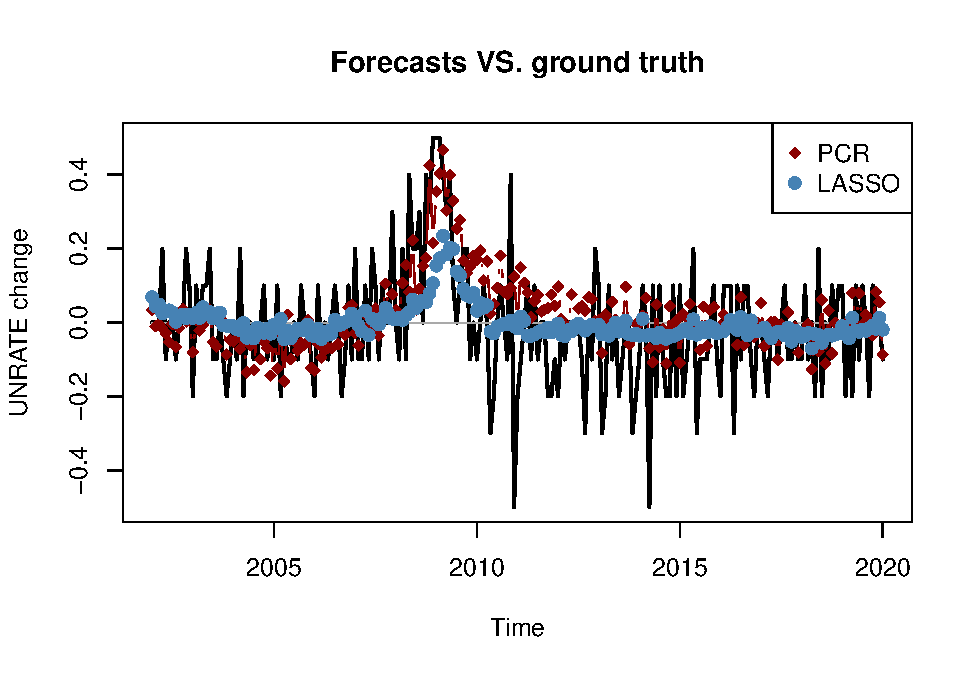
\includegraphics{_main_files/figure-latex/unnamed-chunk-52-1.pdf}

\begin{Shaded}
\begin{Highlighting}[]
\DocumentationTok{\#\# Diebold{-}Mariano test}
\FunctionTok{library}\NormalTok{(forecast)}
\NormalTok{err\_benchmark }\OtherTok{\textless{}{-}}\NormalTok{ data\_test[idx\_eval] }\SpecialCharTok{{-}}\NormalTok{ pred\_mean[idx\_eval]}
\NormalTok{err\_lasso }\OtherTok{\textless{}{-}}\NormalTok{ data\_test[idx\_eval] }\SpecialCharTok{{-}}\NormalTok{ pred\_lasso[idx\_eval]}
\NormalTok{err\_pcr }\OtherTok{\textless{}{-}}\NormalTok{ data\_test[idx\_eval] }\SpecialCharTok{{-}}\NormalTok{ forecast\_list}\SpecialCharTok{$}\NormalTok{pcr[idx\_eval]}

\CommentTok{\# LASSO}
\FunctionTok{dm.test}\NormalTok{(err\_benchmark, err\_lasso, }\AttributeTok{alternative =} \StringTok{"greater"}\NormalTok{)}
\end{Highlighting}
\end{Shaded}

\begin{verbatim}
## 
##  Diebold-Mariano Test
## 
## data:  err_benchmarkerr_lasso
## DM = 3.9017, Forecast horizon = 1, Loss function power = 2, p-value =
## 6.381e-05
## alternative hypothesis: greater
\end{verbatim}

\begin{Shaded}
\begin{Highlighting}[]
\CommentTok{\# PCR}
\FunctionTok{dm.test}\NormalTok{(err\_benchmark, err\_pcr, }\AttributeTok{alternative =} \StringTok{"greater"}\NormalTok{) }
\end{Highlighting}
\end{Shaded}

\begin{verbatim}
## 
##  Diebold-Mariano Test
## 
## data:  err_benchmarkerr_pcr
## DM = 1.0484, Forecast horizon = 1, Loss function power = 2, p-value =
## 0.1478
## alternative hypothesis: greater
\end{verbatim}

\begin{Shaded}
\begin{Highlighting}[]
\DocumentationTok{\#\# plot the cumulated squared errors over time}
\CommentTok{\# compute the (normalized) cumulated squared errors and convert to ts object}
\NormalTok{err2\_benchmark }\OtherTok{\textless{}{-}} \FunctionTok{ts}\NormalTok{(}\FunctionTok{cumsum}\NormalTok{((err\_benchmark)}\SpecialCharTok{\^{}}\DecValTok{2}\NormalTok{), }\AttributeTok{start =} \FunctionTok{c}\NormalTok{(}\DecValTok{2002}\NormalTok{, }\DecValTok{1}\NormalTok{), }\AttributeTok{frequency =} \DecValTok{12}\NormalTok{)}
\NormalTok{err2\_pcr       }\OtherTok{\textless{}{-}} \FunctionTok{ts}\NormalTok{(}\FunctionTok{cumsum}\NormalTok{((err\_pcr)}\SpecialCharTok{\^{}}\DecValTok{2}\NormalTok{), }\AttributeTok{start =} \FunctionTok{c}\NormalTok{(}\DecValTok{2002}\NormalTok{, }\DecValTok{1}\NormalTok{), }\AttributeTok{frequency =} \DecValTok{12}\NormalTok{)}
\NormalTok{err2\_lasso     }\OtherTok{\textless{}{-}} \FunctionTok{ts}\NormalTok{(}\FunctionTok{cumsum}\NormalTok{((err\_lasso)}\SpecialCharTok{\^{}}\DecValTok{2}\NormalTok{), }\AttributeTok{start =} \FunctionTok{c}\NormalTok{(}\DecValTok{2002}\NormalTok{, }\DecValTok{1}\NormalTok{), }\AttributeTok{frequency =} \DecValTok{12}\NormalTok{)}
\NormalTok{err2\_constant  }\OtherTok{\textless{}{-}} \FunctionTok{sum}\NormalTok{(err\_benchmark}\SpecialCharTok{\^{}}\DecValTok{2}\NormalTok{)}
\CommentTok{\# plot}
\FunctionTok{plot.ts}\NormalTok{(err2\_benchmark}\SpecialCharTok{/}\NormalTok{err2\_constant, }\AttributeTok{lwd =} \DecValTok{2}\NormalTok{,}
        \AttributeTok{ylab =} \StringTok{"Cumulated squared errors"}\NormalTok{,}
        \AttributeTok{main =} \StringTok{"Forecast errors over time"}\NormalTok{,}
        \AttributeTok{xlab =} \StringTok{""}\NormalTok{)}
\FunctionTok{lines}\NormalTok{(err2\_pcr}\SpecialCharTok{/}\NormalTok{err2\_constant, }\AttributeTok{col =} \StringTok{"steelblue"}\NormalTok{, }\AttributeTok{lwd =} \DecValTok{2}\NormalTok{)}
\FunctionTok{lines}\NormalTok{(err2\_lasso}\SpecialCharTok{/}\NormalTok{err2\_constant, }\AttributeTok{col =} \StringTok{"darkred"}\NormalTok{, }\AttributeTok{lwd =} \DecValTok{2}\NormalTok{)}
\FunctionTok{rect}\NormalTok{(}\DecValTok{2008}\NormalTok{,}\SpecialCharTok{{-}}\DecValTok{1}\NormalTok{,}\FloatTok{2009.5}\NormalTok{,}\FloatTok{1.5}\NormalTok{,}\AttributeTok{col =} \FunctionTok{rgb}\NormalTok{(}\FloatTok{0.6}\NormalTok{,}\FloatTok{0.1}\NormalTok{,}\FloatTok{0.1}\NormalTok{,}\DecValTok{1}\SpecialCharTok{/}\DecValTok{4}\NormalTok{))}
\FunctionTok{legend}\NormalTok{(}\StringTok{"topleft"}\NormalTok{, }\FunctionTok{c}\NormalTok{(}\StringTok{"Sample mean"}\NormalTok{, }\StringTok{"PCR"}\NormalTok{, }\StringTok{"LASSO"}\NormalTok{), }
       \AttributeTok{col=}\FunctionTok{c}\NormalTok{(}\StringTok{"black"}\NormalTok{, }\StringTok{"steelblue"}\NormalTok{, }\StringTok{"darkred"}\NormalTok{), }\AttributeTok{lwd=}\DecValTok{6}\NormalTok{)}
\end{Highlighting}
\end{Shaded}

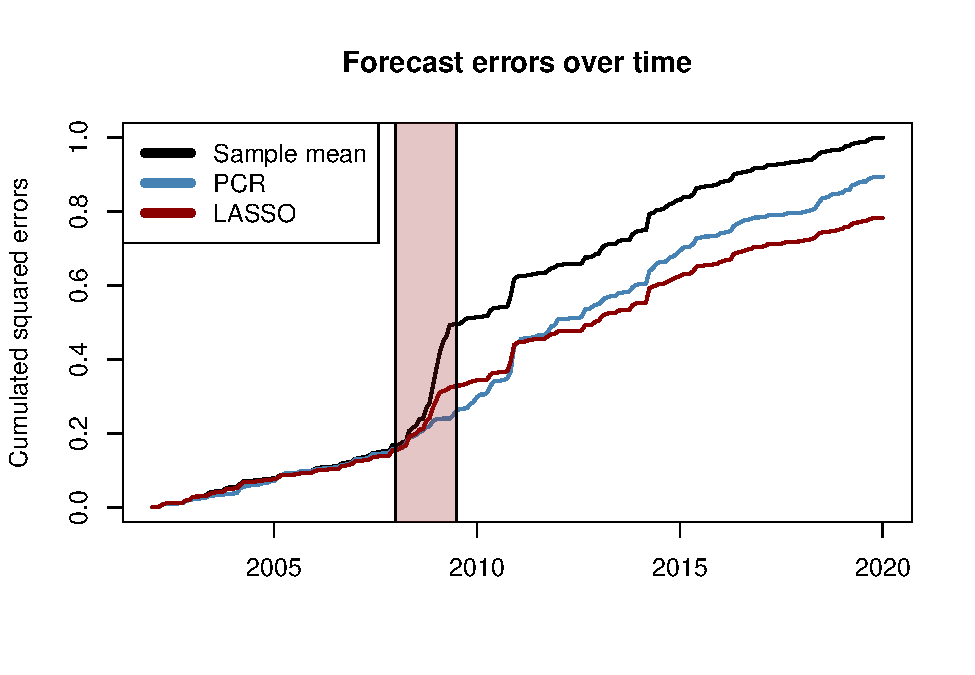
\includegraphics{_main_files/figure-latex/unnamed-chunk-54-1.pdf}

\hypertarget{session04}{%
\chapter{ARMA(1,1) model}\label{session04}}

\hypertarget{mle-for-the-arma11}{%
\section{MLE for the ARMA(1,1)}\label{mle-for-the-arma11}}

In this session we consider the ARMA(1,1) model:

\[
y_t = c + \phi y_{t-1} + \theta \varepsilon_{t-1} + \varepsilon_t, \quad \varepsilon_t \sim WN(0, \sigma^2_\varepsilon)
\]

Below we simulate an ARMA(1,1) model with Gaussian iid noise terms: \(\varepsilon_t \sim \mathcal{N}(0, \sigma^2_\varepsilon)\).

\begin{Shaded}
\begin{Highlighting}[]
\DocumentationTok{\#\# Setup parameters for simulation}
\NormalTok{t\_max }\OtherTok{\textless{}{-}} \DecValTok{800}
\NormalTok{y0    }\OtherTok{\textless{}{-}} \DecValTok{0}
\NormalTok{const }\OtherTok{\textless{}{-}} \DecValTok{0}
\NormalTok{phi   }\OtherTok{\textless{}{-}} \FloatTok{0.9}
\NormalTok{theta }\OtherTok{\textless{}{-}} \SpecialCharTok{{-}}\FloatTok{0.5}
\NormalTok{sigma\_eps }\OtherTok{\textless{}{-}} \DecValTok{1}

\DocumentationTok{\#\# Simulation ARMA(1,1)}
\NormalTok{eps }\OtherTok{\textless{}{-}} \FunctionTok{rnorm}\NormalTok{(t\_max}\SpecialCharTok{+}\DecValTok{1}\NormalTok{, }\AttributeTok{sd =}\NormalTok{ sigma\_eps)}
\NormalTok{y }\OtherTok{\textless{}{-}} \FunctionTok{c}\NormalTok{()}
\NormalTok{y[}\DecValTok{1}\NormalTok{] }\OtherTok{\textless{}{-}}\NormalTok{ y0}
\ControlFlowTok{for}\NormalTok{ (t }\ControlFlowTok{in} \DecValTok{2}\SpecialCharTok{:}\NormalTok{t\_max) \{}
\NormalTok{  y[t] }\OtherTok{\textless{}{-}}\NormalTok{ const }\SpecialCharTok{+}\NormalTok{ phi}\SpecialCharTok{*}\NormalTok{y[t}\DecValTok{{-}1}\NormalTok{] }\SpecialCharTok{+}\NormalTok{ theta}\SpecialCharTok{*}\NormalTok{eps[t}\DecValTok{{-}1}\NormalTok{] }\SpecialCharTok{+}\NormalTok{ eps[t]}
\NormalTok{\}}
\end{Highlighting}
\end{Shaded}

\begin{Shaded}
\begin{Highlighting}[]
\FunctionTok{plot.ts}\NormalTok{(y)}
\end{Highlighting}
\end{Shaded}

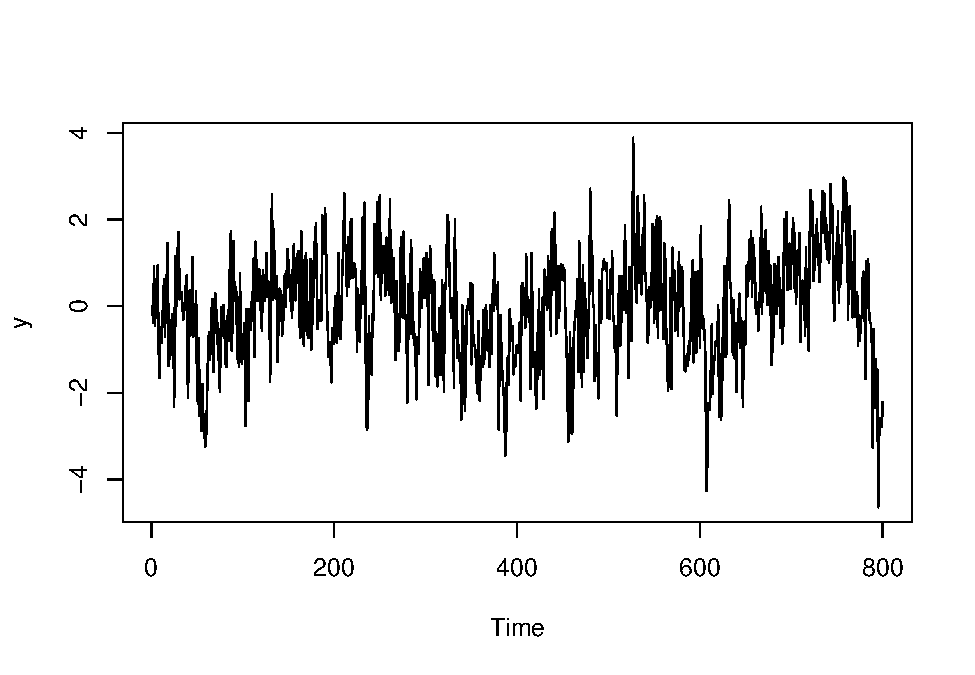
\includegraphics{_main_files/figure-latex/unnamed-chunk-56-1.pdf}

\begin{Shaded}
\begin{Highlighting}[]
\DocumentationTok{\#\# Autocorrelograms}
\FunctionTok{acf}\NormalTok{(y, }\AttributeTok{lwd =} \DecValTok{3}\NormalTok{)}
\end{Highlighting}
\end{Shaded}

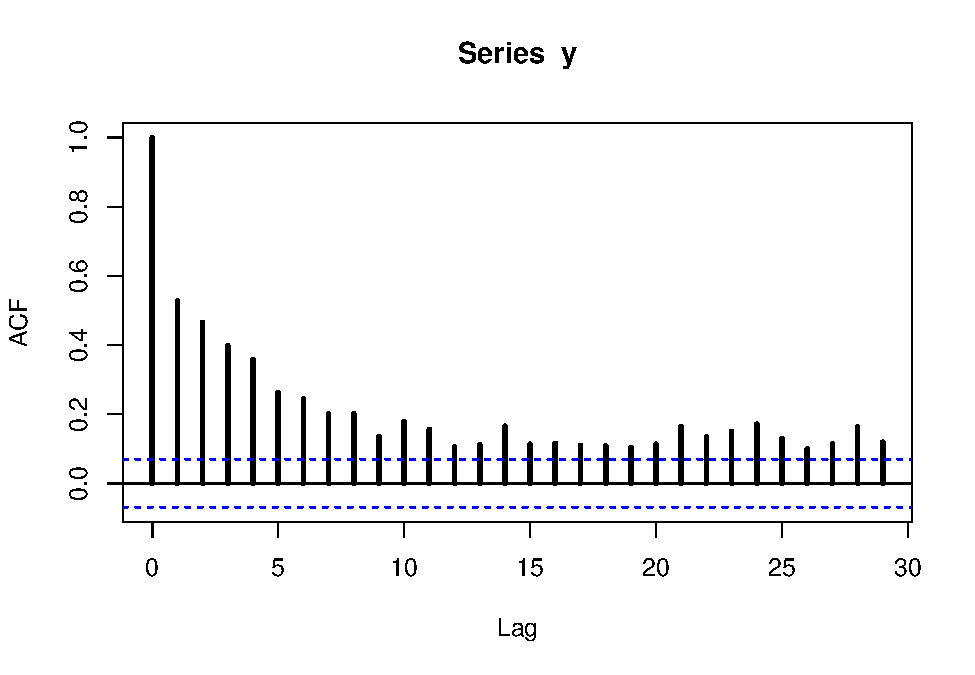
\includegraphics{_main_files/figure-latex/unnamed-chunk-57-1.pdf}

\begin{Shaded}
\begin{Highlighting}[]
\FunctionTok{pacf}\NormalTok{(y, }\AttributeTok{lwd =} \DecValTok{3}\NormalTok{)}
\end{Highlighting}
\end{Shaded}

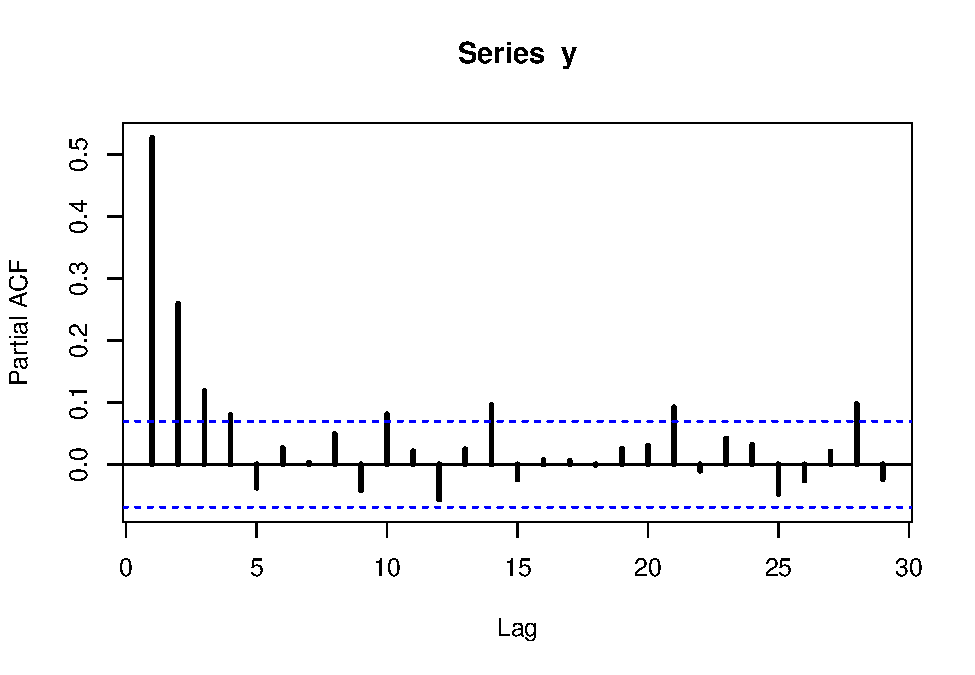
\includegraphics{_main_files/figure-latex/unnamed-chunk-57-2.pdf}

We now turn to estimate the model by maximum likelihood. We can then compare the estimates with the true values of the parameters that we used to simulate the data. Notice that the distribution of observation \(y_t\) given all the information set \(I_{t-1}\) available up to time \(t-1\) is

\[
y_t | I_{t-1} \sim \mathcal{N}(c + \phi y_{t-1} + \theta \varepsilon_{t-1}, \ \sigma^2_\varepsilon).
\]

Let \$ \eta = (c, \phi, \theta, \sigma\^{}2\_\varepsilon)\$ denote the vector of parameters of the model. The \emph{conditional} likelihood can be obtained as:

\[
L(\eta; y_1, \dots, y_T) = \prod_{t=2}^T \frac{1}{\sqrt{2\pi\sigma^2_{\varepsilon}}} \exp\left( -\frac{1}{2\sigma^2_\varepsilon} (y_t - c - \phi y_{t-1} - \theta \varepsilon_{t-1} )^2  \right) 
\]

where the conditioning is on the first observation \(y_1\). Taking the logarithm and defining \(\hat \varepsilon_t = y_t - c - \phi y_{t-1} - \theta \varepsilon_{t-1}\) we get

\[
\ell(\eta ;  y_1, \dots, y_T)  =  - \frac{T-1}{2} \log(2\pi\sigma^2_\varepsilon) - \frac{1}{2\sigma^2_\varepsilon} \sum_{t=2}^T \hat\varepsilon_t^2
\]

The estimate of the innovations can be obtained using a filtering procedure: for a given value of the parameters \(\eta = (c, \phi, \theta, \sigma^2_\varepsilon)\), we set \(\hat\varepsilon_1\) equal to the deviation from the unconditional mean of the first observation, \(\hat\varepsilon_1 = y_1 - \frac{c}{1-\phi}\), and then we compute \(\hat\varepsilon_{t} = y_t - c - \phi y_{t-1} + \theta \hat\varepsilon_{t-1}\) recursively for \(t = 2, \dots, T\). Then we can use the estimated sequence of innovations \(\{\hat\varepsilon_t\}_{t=2}^T\) to evaluate the log-likelihood in \(\eta\).

\begin{Shaded}
\begin{Highlighting}[]
\DocumentationTok{\#\# Estimation: filtering}

\DocumentationTok{\#\# 1{-}step ahead conditional mean of ARMA(1,1) model}
\NormalTok{arma\_filter }\OtherTok{\textless{}{-}} \ControlFlowTok{function}\NormalTok{(x, params)\{}
  \CommentTok{\# get parameters}
\NormalTok{  const }\OtherTok{\textless{}{-}}\NormalTok{ params[}\DecValTok{1}\NormalTok{]}
\NormalTok{  phi }\OtherTok{\textless{}{-}}\NormalTok{ params[}\DecValTok{2}\NormalTok{]}
\NormalTok{  theta }\OtherTok{\textless{}{-}}\NormalTok{ params[}\DecValTok{3}\NormalTok{]}

  \DocumentationTok{\#\# initialize intercept, innovation}
\NormalTok{  mu }\OtherTok{\textless{}{-}} \FunctionTok{rep}\NormalTok{(}\DecValTok{0}\NormalTok{, }\FunctionTok{length}\NormalTok{(x))}
\NormalTok{  mu[}\DecValTok{1}\NormalTok{] }\OtherTok{\textless{}{-}}\NormalTok{ const}\SpecialCharTok{/}\NormalTok{(}\DecValTok{1}\SpecialCharTok{{-}}\NormalTok{phi)}
\NormalTok{  eps }\OtherTok{\textless{}{-}} \FunctionTok{rep}\NormalTok{(}\DecValTok{0}\NormalTok{, }\FunctionTok{length}\NormalTok{(x))}
\NormalTok{  eps[}\DecValTok{1}\NormalTok{] }\OtherTok{\textless{}{-}}\NormalTok{ x[}\DecValTok{1}\NormalTok{] }\SpecialCharTok{{-}}\NormalTok{ mu[}\DecValTok{1}\NormalTok{]}

  \CommentTok{\# filter and innovations}
  \ControlFlowTok{for}\NormalTok{(t }\ControlFlowTok{in} \DecValTok{2}\SpecialCharTok{:}\FunctionTok{length}\NormalTok{(x))\{}
\NormalTok{    mu[t] }\OtherTok{\textless{}{-}}\NormalTok{ const }\SpecialCharTok{+}\NormalTok{ phi}\SpecialCharTok{*}\NormalTok{x[t}\DecValTok{{-}1}\NormalTok{] }\SpecialCharTok{+}\NormalTok{ theta}\SpecialCharTok{*}\NormalTok{eps[t}\DecValTok{{-}1}\NormalTok{]}
\NormalTok{    eps[t] }\OtherTok{\textless{}{-}}\NormalTok{ x[t] }\SpecialCharTok{{-}}\NormalTok{ mu[t]}
\NormalTok{  \}}

  \CommentTok{\# output: estimated innovations}
\NormalTok{  eps}
\NormalTok{\}}
\end{Highlighting}
\end{Shaded}

\begin{Shaded}
\begin{Highlighting}[]
\NormalTok{arma\_loglik }\OtherTok{\textless{}{-}} \ControlFlowTok{function}\NormalTok{(x, params)\{}
  \CommentTok{\# params now include (c, phi, theta, sigma2)}
\NormalTok{  t\_max }\OtherTok{\textless{}{-}} \FunctionTok{length}\NormalTok{(x)}
\NormalTok{  sigma2 }\OtherTok{\textless{}{-}}\NormalTok{ params[}\DecValTok{4}\NormalTok{]}
\NormalTok{  eps }\OtherTok{\textless{}{-}} \FunctionTok{arma\_filter}\NormalTok{(x, params[}\DecValTok{1}\SpecialCharTok{:}\DecValTok{3}\NormalTok{])}

  \CommentTok{\# compute loglik}
\NormalTok{  loglik }\OtherTok{\textless{}{-}} \SpecialCharTok{{-}}\FloatTok{0.5}\SpecialCharTok{*}\NormalTok{t\_max}\SpecialCharTok{*}\FunctionTok{log}\NormalTok{(}\DecValTok{2}\SpecialCharTok{*}\NormalTok{pi}\SpecialCharTok{*}\NormalTok{sigma2) }\SpecialCharTok{{-}}\NormalTok{ (}\DecValTok{1}\SpecialCharTok{/}\NormalTok{(}\DecValTok{2}\SpecialCharTok{*}\NormalTok{sigma2))}\SpecialCharTok{*}\FunctionTok{sum}\NormalTok{(eps}\SpecialCharTok{\^{}}\DecValTok{2}\NormalTok{)}
  
  \CommentTok{\# nlm() minimizes functions {-}{-}\textgreater{} we swap the sign of the log{-}likelihood}
  \CommentTok{\# (max L = min {-}L)}
  \SpecialCharTok{{-}}\NormalTok{loglik}
\NormalTok{\}}
\end{Highlighting}
\end{Shaded}

\begin{Shaded}
\begin{Highlighting}[]
\DocumentationTok{\#\# estimation}
\NormalTok{param\_estim }\OtherTok{\textless{}{-}} \FunctionTok{nlm}\NormalTok{(arma\_loglik, }\AttributeTok{p =} \FunctionTok{c}\NormalTok{(}\DecValTok{0}\NormalTok{, }\FloatTok{0.1}\NormalTok{, }\DecValTok{0}\NormalTok{, }\DecValTok{1}\NormalTok{), }\AttributeTok{x =}\NormalTok{ y)}\SpecialCharTok{$}\NormalTok{estimate}
\end{Highlighting}
\end{Shaded}

\begin{verbatim}
## Warning in nlm(arma_loglik, p = c(0, 0.1, 0, 1), x = y): NA/Inf sostituito da
## valore massimo positivo

## Warning in nlm(arma_loglik, p = c(0, 0.1, 0, 1), x = y): NA/Inf sostituito da
## valore massimo positivo

## Warning in nlm(arma_loglik, p = c(0, 0.1, 0, 1), x = y): NA/Inf sostituito da
## valore massimo positivo
\end{verbatim}

\begin{Shaded}
\begin{Highlighting}[]
\FunctionTok{cbind}\NormalTok{(}\FunctionTok{c}\NormalTok{(const, phi, theta, sigma\_eps), }\FunctionTok{round}\NormalTok{(param\_estim, }\DecValTok{3}\NormalTok{))}
\end{Highlighting}
\end{Shaded}

\begin{verbatim}
##      [,1]   [,2]
## [1,]  0.0 -0.005
## [2,]  0.9  0.873
## [3,] -0.5 -0.515
## [4,]  1.0  1.030
\end{verbatim}

\hypertarget{exercises}{%
\section{Exercises}\label{exercises}}

\textbf{Exercise 1 (LASSO as OLS with thresholding)}

Consider the linear regression model \(y = X\beta + \varepsilon\) with uncorrelated regressors: \(X'X = I_n\), where \(X\in\mathbb{R}^{T\times n}\). Show that the LASSO estimator
\[
\hat\beta^{(\lambda)} = \arg\min_{\beta \in \mathbb{R}^n} \ (y-X\beta)'(y-X\beta) + \lambda ||\beta||_1
\]
can be written as

\[
\hat\beta_j^{(\lambda)} = 
\begin{cases}
\hat\beta_j^{OLS} - \frac{\lambda}{2} & \qquad \text{if} \quad \hat\beta_j^{OLS} >  \frac{\lambda}{2} \\
\hat\beta_j^{OLS} + \frac{\lambda}{2} & \qquad \text{if} \quad \hat\beta_j^{OLS} <  -\frac{\lambda}{2} \\
0 & \qquad \text{if} \quad \hat\beta_j^{OLS} \in  \left[ -\frac{\lambda}{2}, \frac{\lambda}{2} \right]\\
\end{cases}
\]

where \(\hat\beta_j^{OLS}\) denotes the \(j\)-th entry of the OLS estimator and \(j = 1, \dots, n\).

\textbf{Exercise 2 (MA(\(\infty\)) representation of stationary ARMA(1,1))}

Show that the ARMA(1,1) process with \(|\phi| < 1\)

\[
y_t = c + \phi y_{t-1} + \theta \varepsilon_{t-1} + \varepsilon_t, \quad \varepsilon_t \sim WN(0, \sigma^2_\varepsilon)
\]

can be rewritten as

\[
y_t = \mu + \sum_{j=0}^\infty \psi_j \varepsilon_{t-j},
\]

for \(\mu = \frac{c}{1-\phi}\), \(\psi_0 = 1\), \(\psi_j = (\phi + \theta)\phi^{j-1}\).

\textbf{Exercise 3 (autocovariance function of the ARMA(1,1))}

Show that the covariance function \(\gamma(k) = \text{cov}(y_t, y_{t-k})\) of the ARMA(1,1) process

\[
y_t = c + \phi y_{t-1} + \theta \varepsilon_{t-1} + \varepsilon_t, \quad \varepsilon_t \sim WN(0, \sigma^2_\varepsilon)
\]

with \(|\phi < 1|\) can be written as

\[
\gamma(k) = 
\begin{cases}
\sigma^2_\varepsilon \left(1 + \frac{(\phi+\theta)^2}{1-\phi^2}\right) & \qquad \text{for} \quad k=0 \\[1em]
\sigma^2_\varepsilon \left(\phi+\theta + \frac{(\phi+\theta)^2\phi}{1-\phi^2}\right) & \qquad \text{for} \quad k=1 \\[1em]
\phi^{k-1} \ \gamma(1) &  \qquad \text{for} \quad k>1 
\end{cases}
\]

\emph{Hint}: you may use the fact that for a linear time series \(y_t = \mu + \sum_{j=0}^\infty \psi_j \varepsilon_{t-j}\) the autocovariance function is given by

\[
\gamma(k) = \sigma^2_\varepsilon \sum_{j=k}^\infty \psi_j \psi_{j-k},
\]

provided that \(\sum_{j=0}^{\infty} \psi_j^2 < \infty\).

\hypertarget{session05}{%
\chapter{ARMA models in practice}\label{session05}}

\begin{Shaded}
\begin{Highlighting}[]
\DocumentationTok{\#\# load libraries}
\FunctionTok{library}\NormalTok{(moments)}

\DocumentationTok{\#\# function to plot time series}
\NormalTok{myplot }\OtherTok{\textless{}{-}} \ControlFlowTok{function}\NormalTok{( dates , y , }\AttributeTok{col=}\StringTok{\textquotesingle{}darkblue\textquotesingle{}}\NormalTok{ , }\AttributeTok{t=}\StringTok{\textquotesingle{}l\textquotesingle{}}\NormalTok{ , }\AttributeTok{lwd=}\DecValTok{2}\NormalTok{ , }\AttributeTok{ylim=}\ConstantTok{NULL}\NormalTok{ , }\AttributeTok{main=}\ConstantTok{NULL}\NormalTok{ )\{}
  \ControlFlowTok{if}\NormalTok{( }\FunctionTok{is.null}\NormalTok{(main) )\{ }\FunctionTok{par}\NormalTok{( }\AttributeTok{mar=}\FunctionTok{c}\NormalTok{(}\DecValTok{2}\NormalTok{,}\DecValTok{2}\NormalTok{,}\FloatTok{0.1}\NormalTok{,}\FloatTok{0.1}\NormalTok{) ) \}}
  \FunctionTok{plot}\NormalTok{( dates , y , }\AttributeTok{t=}\NormalTok{t , }\AttributeTok{col=}\NormalTok{col , }\AttributeTok{lwd=}\NormalTok{lwd , }\AttributeTok{axes=}\NormalTok{F , }\AttributeTok{xlab=}\StringTok{\textquotesingle{}\textquotesingle{}}\NormalTok{ , }\AttributeTok{ylab=}\StringTok{\textquotesingle{}\textquotesingle{}}\NormalTok{ , }\AttributeTok{xaxs=}\StringTok{"i"}\NormalTok{ , }\AttributeTok{ylim=}\NormalTok{ylim , }\AttributeTok{main=}\NormalTok{main )}
\NormalTok{  xticks }\OtherTok{\textless{}{-}} \FunctionTok{axis.Date}\NormalTok{(}\DecValTok{1}\NormalTok{, }\AttributeTok{x=}\NormalTok{dates, }\AttributeTok{at=}\FunctionTok{seq}\NormalTok{(dates[}\DecValTok{1}\NormalTok{], dates[}\FunctionTok{length}\NormalTok{(dates)], }\StringTok{"year"}\NormalTok{) , }\AttributeTok{lwd=}\DecValTok{0}\NormalTok{, }\AttributeTok{lwd.tick=}\DecValTok{1}\NormalTok{, }\AttributeTok{tck=}\FloatTok{0.02}\NormalTok{)}
\NormalTok{  yticks }\OtherTok{\textless{}{-}} \FunctionTok{axis}\NormalTok{(}\DecValTok{2}\NormalTok{ , }\AttributeTok{lwd=}\DecValTok{0}\NormalTok{, }\AttributeTok{lwd.tick=}\DecValTok{1}\NormalTok{, }\AttributeTok{tck=}\FloatTok{0.02}\NormalTok{)}
  \FunctionTok{axis.Date}\NormalTok{(}\DecValTok{3}\NormalTok{, }\AttributeTok{x=}\NormalTok{dates, }\AttributeTok{at=}\FunctionTok{seq}\NormalTok{(dates[}\DecValTok{1}\NormalTok{], dates[}\FunctionTok{length}\NormalTok{(dates)], }\StringTok{"year"}\NormalTok{), }\AttributeTok{lwd=}\DecValTok{0}\NormalTok{, }\AttributeTok{lwd.tick=}\DecValTok{1}\NormalTok{, }\AttributeTok{tck=}\FloatTok{0.02}\NormalTok{, }\AttributeTok{lab=}\NormalTok{F)}
  \FunctionTok{axis}\NormalTok{(}\DecValTok{4}\NormalTok{, }\AttributeTok{lwd=}\DecValTok{0}\NormalTok{, }\AttributeTok{lwd.tick=}\DecValTok{1}\NormalTok{, }\AttributeTok{tck=}\FloatTok{0.02}\NormalTok{, }\AttributeTok{lab=}\NormalTok{F)}
  \FunctionTok{abline}\NormalTok{( }\AttributeTok{h=}\NormalTok{yticks , }\AttributeTok{lty=}\DecValTok{3}\NormalTok{ )}
  \FunctionTok{abline}\NormalTok{( }\AttributeTok{v=}\NormalTok{xticks , }\AttributeTok{lty=}\DecValTok{3}\NormalTok{ )}
  \FunctionTok{box}\NormalTok{()}
\NormalTok{\}}
\end{Highlighting}
\end{Shaded}

\hypertarget{forecasting-the-u.s.-gdp-growth}{%
\section{Forecasting the U.S. GDP growth}\label{forecasting-the-u.s.-gdp-growth}}

In this session we consider an application of ARMA models to forecasting the U.S. GDP growth rates.

\begin{Shaded}
\begin{Highlighting}[]
\DocumentationTok{\#\# Load U.S. GDP growth rate}
\NormalTok{D }\OtherTok{\textless{}{-}} \FunctionTok{read.table}\NormalTok{(}\StringTok{\textquotesingle{}../data/gdp{-}us{-}grate.csv\textquotesingle{}}\NormalTok{)}
\NormalTok{dates }\OtherTok{\textless{}{-}} \FunctionTok{as.Date}\NormalTok{(}\FunctionTok{as.character}\NormalTok{(D[,}\DecValTok{1}\NormalTok{]),}\StringTok{\textquotesingle{}\%Y{-}\%m{-}\%d\textquotesingle{}}\NormalTok{)}

\DocumentationTok{\#\# Setup }
\NormalTok{H }\OtherTok{\textless{}{-}} \DecValTok{6}   \CommentTok{\# predict 1,2,...,H steps ahead}
\NormalTok{N }\OtherTok{\textless{}{-}} \FunctionTok{nrow}\NormalTok{(D)}\SpecialCharTok{{-}}\DecValTok{6}
\NormalTok{y }\OtherTok{\textless{}{-}}\NormalTok{ D[}\DecValTok{1}\SpecialCharTok{:}\NormalTok{N,}\DecValTok{2}\NormalTok{]}
\NormalTok{y.out }\OtherTok{\textless{}{-}}\NormalTok{D[(N}\SpecialCharTok{+}\DecValTok{1}\NormalTok{)}\SpecialCharTok{:}\NormalTok{(N}\SpecialCharTok{+}\NormalTok{H),}\DecValTok{2}\NormalTok{]}
\end{Highlighting}
\end{Shaded}

\begin{Shaded}
\begin{Highlighting}[]
\CommentTok{\# LBQ Test for autocorrelation}
\FunctionTok{Box.test}\NormalTok{( y, }\AttributeTok{lag=}\DecValTok{22}\NormalTok{ , }\AttributeTok{type=}\StringTok{"Ljung{-}Box"}\NormalTok{)}
\end{Highlighting}
\end{Shaded}

\begin{verbatim}
## 
##  Box-Ljung test
## 
## data:  y
## X-squared = 82.561, df = 22, p-value = 6.112e-09
\end{verbatim}

\begin{Shaded}
\begin{Highlighting}[]
\CommentTok{\# ACF \& PACF}
\FunctionTok{par}\NormalTok{( }\AttributeTok{mar=}\FunctionTok{c}\NormalTok{(}\DecValTok{2}\NormalTok{,}\DecValTok{2}\NormalTok{,}\DecValTok{1}\NormalTok{,}\DecValTok{1}\NormalTok{) , }\AttributeTok{mfrow=}\FunctionTok{c}\NormalTok{(}\DecValTok{2}\NormalTok{,}\DecValTok{1}\NormalTok{) )}
\FunctionTok{acf}\NormalTok{( y , }\AttributeTok{ylim=}\FunctionTok{c}\NormalTok{(}\SpecialCharTok{{-}}\FloatTok{0.2}\NormalTok{,}\DecValTok{1}\NormalTok{) , }\AttributeTok{lwd=}\DecValTok{5}\NormalTok{ , }\AttributeTok{xlim=}\FunctionTok{c}\NormalTok{(}\DecValTok{0}\NormalTok{,}\DecValTok{25}\NormalTok{) , }\AttributeTok{col=}\StringTok{\textquotesingle{}darkorange2\textquotesingle{}}\NormalTok{ , }\AttributeTok{tck=}\FloatTok{0.02}\NormalTok{)}
\FunctionTok{legend}\NormalTok{(}\StringTok{\textquotesingle{}topright\textquotesingle{}}\NormalTok{,}\FunctionTok{c}\NormalTok{(}\StringTok{\textquotesingle{}ACF\textquotesingle{}}\NormalTok{),}\AttributeTok{col=}\FunctionTok{c}\NormalTok{(}\StringTok{\textquotesingle{}darkorange2\textquotesingle{}}\NormalTok{),}\AttributeTok{lwd=}\DecValTok{3}\NormalTok{)}
\FunctionTok{pacf}\NormalTok{( y , }\AttributeTok{ylim=}\FunctionTok{c}\NormalTok{(}\SpecialCharTok{{-}}\FloatTok{0.2}\NormalTok{,}\DecValTok{1}\NormalTok{) , }\AttributeTok{lwd=}\DecValTok{5}\NormalTok{ , }\AttributeTok{xlim=}\FunctionTok{c}\NormalTok{(}\DecValTok{0}\NormalTok{,}\DecValTok{25}\NormalTok{) , }\AttributeTok{col=}\StringTok{\textquotesingle{}darkorange2\textquotesingle{}}\NormalTok{ , }\AttributeTok{tck=}\FloatTok{0.02}\NormalTok{)}
\FunctionTok{legend}\NormalTok{(}\StringTok{\textquotesingle{}topright\textquotesingle{}}\NormalTok{,}\FunctionTok{c}\NormalTok{(}\StringTok{\textquotesingle{}PACF\textquotesingle{}}\NormalTok{),}\AttributeTok{col=}\FunctionTok{c}\NormalTok{(}\StringTok{\textquotesingle{}darkorange2\textquotesingle{}}\NormalTok{),}\AttributeTok{lwd=}\DecValTok{3}\NormalTok{)}
\end{Highlighting}
\end{Shaded}

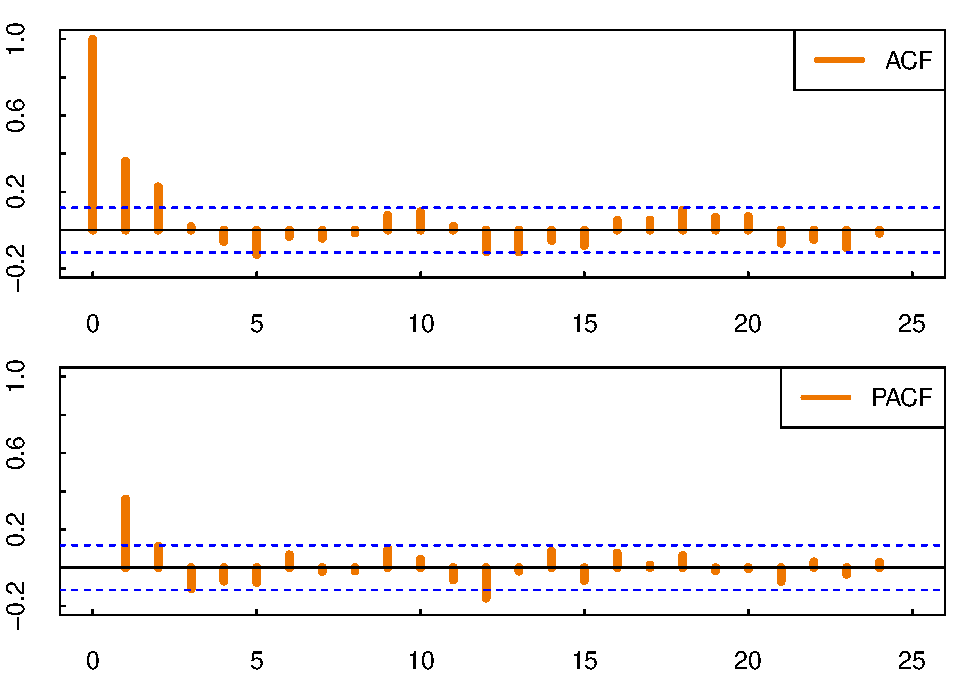
\includegraphics{_main_files/figure-latex/unnamed-chunk-63-1.pdf}

\hypertarget{estimation}{%
\subsubsection*{Estimation}\label{estimation}}
\addcontentsline{toc}{subsubsection}{Estimation}

\begin{Shaded}
\begin{Highlighting}[]
\NormalTok{ar1    }\OtherTok{\textless{}{-}} \FunctionTok{arima}\NormalTok{(y,}\AttributeTok{order=}\FunctionTok{c}\NormalTok{(}\DecValTok{1}\NormalTok{,}\DecValTok{0}\NormalTok{,}\DecValTok{0}\NormalTok{))}
\NormalTok{ma1    }\OtherTok{\textless{}{-}} \FunctionTok{arima}\NormalTok{(y,}\AttributeTok{order=}\FunctionTok{c}\NormalTok{(}\DecValTok{0}\NormalTok{,}\DecValTok{0}\NormalTok{,}\DecValTok{1}\NormalTok{))}
\NormalTok{ma2    }\OtherTok{\textless{}{-}} \FunctionTok{arima}\NormalTok{(y,}\AttributeTok{order=}\FunctionTok{c}\NormalTok{(}\DecValTok{0}\NormalTok{,}\DecValTok{0}\NormalTok{,}\DecValTok{2}\NormalTok{))}
\NormalTok{arma11 }\OtherTok{\textless{}{-}} \FunctionTok{arima}\NormalTok{(y,}\AttributeTok{order=}\FunctionTok{c}\NormalTok{(}\DecValTok{1}\NormalTok{,}\DecValTok{0}\NormalTok{,}\DecValTok{1}\NormalTok{))}

\CommentTok{\# Information criteria}
\NormalTok{ar1\_aic    }\OtherTok{\textless{}{-}}\NormalTok{ (}\SpecialCharTok{{-}}\DecValTok{2}\SpecialCharTok{*}\NormalTok{ar1}\SpecialCharTok{$}\NormalTok{loglik}\SpecialCharTok{+}\DecValTok{2}\SpecialCharTok{*}\DecValTok{3}\NormalTok{)}\SpecialCharTok{/}\NormalTok{N     }\CommentTok{\# (constant, phi, sigma\_e)}
\NormalTok{ma1\_aic    }\OtherTok{\textless{}{-}}\NormalTok{ (}\SpecialCharTok{{-}}\DecValTok{2}\SpecialCharTok{*}\NormalTok{ma1}\SpecialCharTok{$}\NormalTok{loglik}\SpecialCharTok{+}\DecValTok{2}\SpecialCharTok{*}\DecValTok{3}\NormalTok{)}\SpecialCharTok{/}\NormalTok{N     }\CommentTok{\# (constant, theta, sigma\_e)}
\NormalTok{ma2\_aic    }\OtherTok{\textless{}{-}}\NormalTok{ (}\SpecialCharTok{{-}}\DecValTok{2}\SpecialCharTok{*}\NormalTok{ma2}\SpecialCharTok{$}\NormalTok{loglik}\SpecialCharTok{+}\DecValTok{2}\SpecialCharTok{*}\DecValTok{4}\NormalTok{)}\SpecialCharTok{/}\NormalTok{N     }\CommentTok{\# (constant, theta1, theta2, sigma\_e)}
\NormalTok{arma11\_aic }\OtherTok{\textless{}{-}}\NormalTok{ (}\SpecialCharTok{{-}}\DecValTok{2}\SpecialCharTok{*}\NormalTok{arma11}\SpecialCharTok{$}\NormalTok{loglik}\SpecialCharTok{+}\DecValTok{2}\SpecialCharTok{*}\DecValTok{4}\NormalTok{)}\SpecialCharTok{/}\NormalTok{N  }\CommentTok{\# (constant, phi, theta, sigma\_e)}

\NormalTok{ar1\_bic    }\OtherTok{\textless{}{-}}\NormalTok{ (}\SpecialCharTok{{-}}\DecValTok{2}\SpecialCharTok{*}\NormalTok{ar1}\SpecialCharTok{$}\NormalTok{loglik}\SpecialCharTok{+}\FunctionTok{log}\NormalTok{(N)}\SpecialCharTok{*}\DecValTok{3}\NormalTok{)}\SpecialCharTok{/}\NormalTok{N}
\NormalTok{ma1\_bic    }\OtherTok{\textless{}{-}}\NormalTok{ (}\SpecialCharTok{{-}}\DecValTok{2}\SpecialCharTok{*}\NormalTok{ma1}\SpecialCharTok{$}\NormalTok{loglik}\SpecialCharTok{+}\FunctionTok{log}\NormalTok{(N)}\SpecialCharTok{*}\DecValTok{3}\NormalTok{)}\SpecialCharTok{/}\NormalTok{N}
\NormalTok{ma2\_bic    }\OtherTok{\textless{}{-}}\NormalTok{ (}\SpecialCharTok{{-}}\DecValTok{2}\SpecialCharTok{*}\NormalTok{ma2}\SpecialCharTok{$}\NormalTok{loglik}\SpecialCharTok{+}\FunctionTok{log}\NormalTok{(N)}\SpecialCharTok{*}\DecValTok{4}\NormalTok{)}\SpecialCharTok{/}\NormalTok{N}
\NormalTok{arma11\_bic }\OtherTok{\textless{}{-}}\NormalTok{ (}\SpecialCharTok{{-}}\DecValTok{2}\SpecialCharTok{*}\NormalTok{arma11}\SpecialCharTok{$}\NormalTok{loglik}\SpecialCharTok{+}\FunctionTok{log}\NormalTok{(N)}\SpecialCharTok{*}\DecValTok{4}\NormalTok{)}\SpecialCharTok{/}\NormalTok{N}

\DocumentationTok{\#\# table of likelihood and ICs}
\NormalTok{tab1 }\OtherTok{\textless{}{-}} \FunctionTok{round}\NormalTok{( }\FunctionTok{rbind}\NormalTok{( }\FunctionTok{c}\NormalTok{(ar1}\SpecialCharTok{$}\NormalTok{loglik,ma1}\SpecialCharTok{$}\NormalTok{loglik.ma2}\SpecialCharTok{$}\NormalTok{loglik,arma11}\SpecialCharTok{$}\NormalTok{loglik), }
              \FunctionTok{c}\NormalTok{(ar1\_aic,ma1\_aic,ma2\_aic,arma11\_aic) , }
              \FunctionTok{c}\NormalTok{(ar1\_bic,ma1\_bic,ma2\_bic,arma11\_bic) ) ,  }\DecValTok{3}\NormalTok{ )}
\FunctionTok{row.names}\NormalTok{(tab1) }\OtherTok{\textless{}{-}} \FunctionTok{c}\NormalTok{(}\StringTok{"loglik"}\NormalTok{, }\StringTok{"AIC"}\NormalTok{, }\StringTok{"BIC"}\NormalTok{)}
\FunctionTok{colnames}\NormalTok{(tab1)  }\OtherTok{\textless{}{-}} \FunctionTok{c}\NormalTok{(}\StringTok{"AR(1)"}\NormalTok{, }\StringTok{"MA(1)"}\NormalTok{, }\StringTok{"MA(2)"}\NormalTok{, }\StringTok{"ARMA(1,1)"}\NormalTok{)}
\NormalTok{tab1}
\end{Highlighting}
\end{Shaded}

\begin{verbatim}
##           AR(1)    MA(1)    MA(2) ARMA(1,1)
## loglik -747.736 -746.702 -747.736  -746.702
## AIC       5.382    5.419    5.371     5.381
## BIC       5.421    5.458    5.423     5.433
\end{verbatim}

\hypertarget{forecasting}{%
\subsubsection*{Forecasting}\label{forecasting}}
\addcontentsline{toc}{subsubsection}{Forecasting}

\begin{Shaded}
\begin{Highlighting}[]
\DocumentationTok{\#\# get forecasts}
\NormalTok{ar1\_pred    }\OtherTok{\textless{}{-}} \FunctionTok{predict}\NormalTok{(ar1, }\AttributeTok{n.ahead=}\NormalTok{H)}
\NormalTok{ma1\_pred    }\OtherTok{\textless{}{-}} \FunctionTok{predict}\NormalTok{(ma1, }\AttributeTok{n.ahead=}\NormalTok{H)}
\NormalTok{ma2\_pred    }\OtherTok{\textless{}{-}} \FunctionTok{predict}\NormalTok{(ma2, }\AttributeTok{n.ahead=}\NormalTok{H)}
\NormalTok{arma11\_pred }\OtherTok{\textless{}{-}} \FunctionTok{predict}\NormalTok{(arma11, }\AttributeTok{n.ahead=}\NormalTok{H)}

\DocumentationTok{\#\# get fitted values}
\NormalTok{ar1\_mu     }\OtherTok{\textless{}{-}}\NormalTok{ y}\SpecialCharTok{{-}}\NormalTok{ar1}\SpecialCharTok{$}\NormalTok{residuals}
\NormalTok{ma1\_mu     }\OtherTok{\textless{}{-}}\NormalTok{ y}\SpecialCharTok{{-}}\NormalTok{ma1}\SpecialCharTok{$}\NormalTok{residuals}
\NormalTok{ma2\_mu     }\OtherTok{\textless{}{-}}\NormalTok{ y}\SpecialCharTok{{-}}\NormalTok{ma2}\SpecialCharTok{$}\NormalTok{residuals}
\NormalTok{arma11\_mu  }\OtherTok{\textless{}{-}}\NormalTok{ y}\SpecialCharTok{{-}}\NormalTok{arma11}\SpecialCharTok{$}\NormalTok{residuals}

\DocumentationTok{\#\# compute RMSE}
\NormalTok{rmse }\OtherTok{\textless{}{-}} \ControlFlowTok{function}\NormalTok{(y, f) \{}\FunctionTok{sqrt}\NormalTok{(}\FunctionTok{mean}\NormalTok{((y}\SpecialCharTok{{-}}\FunctionTok{as.numeric}\NormalTok{(f))}\SpecialCharTok{\^{}}\DecValTok{2}\NormalTok{))\}}
\NormalTok{ar1\_mse    }\OtherTok{\textless{}{-}}\FunctionTok{rmse}\NormalTok{(y.out, ar1\_pred}\SpecialCharTok{$}\NormalTok{pred)}
\NormalTok{ma1\_mse    }\OtherTok{\textless{}{-}}\FunctionTok{rmse}\NormalTok{(y.out, ma1\_pred}\SpecialCharTok{$}\NormalTok{pred)}
\NormalTok{ma2\_mse    }\OtherTok{\textless{}{-}}\FunctionTok{rmse}\NormalTok{(y.out, ma2\_pred}\SpecialCharTok{$}\NormalTok{pred)}
\NormalTok{arma11\_mse }\OtherTok{\textless{}{-}}\FunctionTok{rmse}\NormalTok{(y.out, arma11\_pred}\SpecialCharTok{$}\NormalTok{pred)}

\DocumentationTok{\#\# Plot}
\FunctionTok{par}\NormalTok{(}\AttributeTok{mfrow =} \FunctionTok{c}\NormalTok{(}\DecValTok{1}\NormalTok{,}\DecValTok{2}\NormalTok{))}

\FunctionTok{myplot}\NormalTok{( dates[(N}\DecValTok{{-}10}\NormalTok{)}\SpecialCharTok{:}\NormalTok{(N}\SpecialCharTok{+}\NormalTok{H)] , }\FunctionTok{c}\NormalTok{(y[(N}\DecValTok{{-}10}\NormalTok{)}\SpecialCharTok{:}\NormalTok{N], y.out) , }\AttributeTok{t=}\StringTok{\textquotesingle{}b\textquotesingle{}}\NormalTok{, }\AttributeTok{main=}\FunctionTok{sprintf}\NormalTok{(}\StringTok{\textquotesingle{}AR(1) RMSE \%3.3f\textquotesingle{}}\NormalTok{,ar1\_mse) , }\AttributeTok{ylim=}\FunctionTok{c}\NormalTok{(}\DecValTok{0}\NormalTok{,}\DecValTok{7}\NormalTok{) , }\AttributeTok{col=}\StringTok{\textquotesingle{}darkorange\textquotesingle{}}\NormalTok{ ) }
\FunctionTok{abline}\NormalTok{( }\AttributeTok{v=}\NormalTok{dates[N] , }\AttributeTok{lwd=}\DecValTok{2}\NormalTok{ )}
\FunctionTok{abline}\NormalTok{( }\AttributeTok{h=}\NormalTok{ar1}\SpecialCharTok{$}\NormalTok{coef[}\StringTok{\textquotesingle{}intercept\textquotesingle{}}\NormalTok{] , }\AttributeTok{lwd=}\DecValTok{2}\NormalTok{ )}
\FunctionTok{lines}\NormalTok{( dates[(N}\DecValTok{{-}10}\NormalTok{)}\SpecialCharTok{:}\NormalTok{N] , ar1\_mu[(N}\DecValTok{{-}10}\NormalTok{)}\SpecialCharTok{:}\NormalTok{N] , }\AttributeTok{t=}\StringTok{\textquotesingle{}l\textquotesingle{}}\NormalTok{ , }\AttributeTok{lwd=}\DecValTok{2}\NormalTok{ , }\AttributeTok{col=}\StringTok{\textquotesingle{}blue3\textquotesingle{}}\NormalTok{ )}
\FunctionTok{lines}\NormalTok{( dates[(N}\SpecialCharTok{+}\DecValTok{1}\NormalTok{)}\SpecialCharTok{:}\NormalTok{(N}\SpecialCharTok{+}\NormalTok{H)] , }\FunctionTok{as.numeric}\NormalTok{(ar1\_pred}\SpecialCharTok{$}\NormalTok{pred)  , }\AttributeTok{t=}\StringTok{\textquotesingle{}b\textquotesingle{}}\NormalTok{ , }\AttributeTok{lwd=}\DecValTok{2}\NormalTok{ , }\AttributeTok{col=}\StringTok{\textquotesingle{}blue3\textquotesingle{}}\NormalTok{ )}

\FunctionTok{myplot}\NormalTok{( dates[(N}\DecValTok{{-}10}\NormalTok{)}\SpecialCharTok{:}\NormalTok{(N}\SpecialCharTok{+}\NormalTok{H)] , }\FunctionTok{c}\NormalTok{(y[(N}\DecValTok{{-}10}\NormalTok{)}\SpecialCharTok{:}\NormalTok{N], y.out) , }\AttributeTok{t=}\StringTok{\textquotesingle{}b\textquotesingle{}}\NormalTok{ , }\AttributeTok{main=}\FunctionTok{sprintf}\NormalTok{(}\StringTok{\textquotesingle{}ARMA(1,1) RMSE \%3.3f\textquotesingle{}}\NormalTok{,arma11\_mse) , }\AttributeTok{ylim=}\FunctionTok{c}\NormalTok{(}\DecValTok{0}\NormalTok{,}\DecValTok{7}\NormalTok{) , }\AttributeTok{col=}\StringTok{\textquotesingle{}darkorange\textquotesingle{}}\NormalTok{ ) }
\FunctionTok{abline}\NormalTok{( }\AttributeTok{v=}\NormalTok{dates[N] , }\AttributeTok{lwd=}\DecValTok{2}\NormalTok{ )}
\FunctionTok{abline}\NormalTok{( }\AttributeTok{h=}\NormalTok{arma11}\SpecialCharTok{$}\NormalTok{coef[}\StringTok{\textquotesingle{}intercept\textquotesingle{}}\NormalTok{] , }\AttributeTok{lwd=}\DecValTok{2}\NormalTok{ )}
\FunctionTok{lines}\NormalTok{( dates[(N}\DecValTok{{-}10}\NormalTok{)}\SpecialCharTok{:}\NormalTok{N] , arma11\_mu[(N}\DecValTok{{-}10}\NormalTok{)}\SpecialCharTok{:}\NormalTok{N] , }\AttributeTok{t=}\StringTok{\textquotesingle{}l\textquotesingle{}}\NormalTok{ , }\AttributeTok{lwd=}\DecValTok{2}\NormalTok{ , }\AttributeTok{col=}\StringTok{\textquotesingle{}blue3\textquotesingle{}}\NormalTok{ )}
\FunctionTok{lines}\NormalTok{( dates[(N}\SpecialCharTok{+}\DecValTok{1}\NormalTok{)}\SpecialCharTok{:}\NormalTok{(N}\SpecialCharTok{+}\NormalTok{H)] , }\FunctionTok{as.numeric}\NormalTok{(arma11\_pred}\SpecialCharTok{$}\NormalTok{pred)  , }\AttributeTok{t=}\StringTok{\textquotesingle{}b\textquotesingle{}}\NormalTok{ , }\AttributeTok{lwd=}\DecValTok{2}\NormalTok{ , }\AttributeTok{col=}\StringTok{\textquotesingle{}blue3\textquotesingle{}}\NormalTok{ )}
\end{Highlighting}
\end{Shaded}

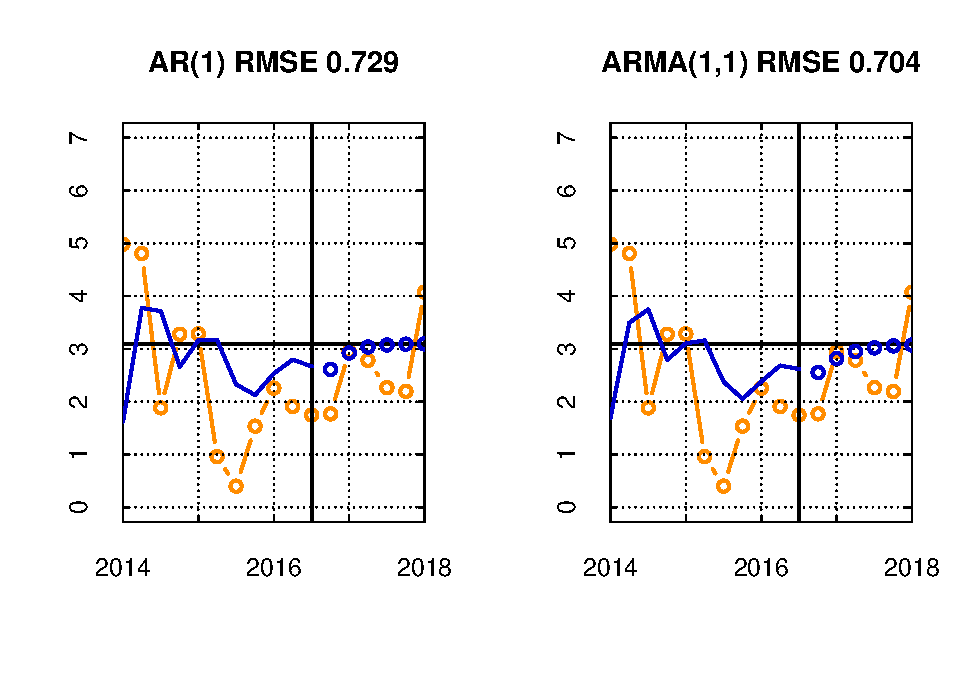
\includegraphics{_main_files/figure-latex/unnamed-chunk-65-1.pdf}

\begin{Shaded}
\begin{Highlighting}[]
\FunctionTok{par}\NormalTok{(}\AttributeTok{mfrow =} \FunctionTok{c}\NormalTok{(}\DecValTok{1}\NormalTok{,}\DecValTok{2}\NormalTok{))}

\FunctionTok{myplot}\NormalTok{( dates[(N}\DecValTok{{-}10}\NormalTok{)}\SpecialCharTok{:}\NormalTok{(N}\SpecialCharTok{+}\NormalTok{H)] , }\FunctionTok{c}\NormalTok{(y[(N}\DecValTok{{-}10}\NormalTok{)}\SpecialCharTok{:}\NormalTok{N], y.out) , }\AttributeTok{t=}\StringTok{\textquotesingle{}b\textquotesingle{}}\NormalTok{, }\AttributeTok{main=}\FunctionTok{sprintf}\NormalTok{(}\StringTok{\textquotesingle{}MA(2) RMSE \%3.3f\textquotesingle{}}\NormalTok{,ma2\_mse) , }\AttributeTok{ylim=}\FunctionTok{c}\NormalTok{(}\DecValTok{0}\NormalTok{,}\DecValTok{7}\NormalTok{) , }\AttributeTok{col=}\StringTok{\textquotesingle{}darkorange\textquotesingle{}}\NormalTok{ ) }
\FunctionTok{abline}\NormalTok{( }\AttributeTok{v=}\NormalTok{dates[N] , }\AttributeTok{lwd=}\DecValTok{2}\NormalTok{ )}
\FunctionTok{abline}\NormalTok{( }\AttributeTok{h=}\NormalTok{ma2}\SpecialCharTok{$}\NormalTok{coef[}\StringTok{\textquotesingle{}intercept\textquotesingle{}}\NormalTok{] , }\AttributeTok{lwd=}\DecValTok{2}\NormalTok{ )}
\FunctionTok{lines}\NormalTok{( dates[(N}\DecValTok{{-}10}\NormalTok{)}\SpecialCharTok{:}\NormalTok{N] , ma2\_mu[(N}\DecValTok{{-}10}\NormalTok{)}\SpecialCharTok{:}\NormalTok{N] , }\AttributeTok{t=}\StringTok{\textquotesingle{}l\textquotesingle{}}\NormalTok{ , }\AttributeTok{lwd=}\DecValTok{2}\NormalTok{ , }\AttributeTok{col=}\StringTok{\textquotesingle{}blue3\textquotesingle{}}\NormalTok{ )}
\FunctionTok{lines}\NormalTok{( dates[(N}\SpecialCharTok{+}\DecValTok{1}\NormalTok{)}\SpecialCharTok{:}\NormalTok{(N}\SpecialCharTok{+}\NormalTok{H)] , }\FunctionTok{as.numeric}\NormalTok{(ma2\_pred}\SpecialCharTok{$}\NormalTok{pred)  , }\AttributeTok{t=}\StringTok{\textquotesingle{}b\textquotesingle{}}\NormalTok{ , }\AttributeTok{lwd=}\DecValTok{2}\NormalTok{ , }\AttributeTok{col=}\StringTok{\textquotesingle{}blue3\textquotesingle{}}\NormalTok{ )}

\FunctionTok{myplot}\NormalTok{( dates[(N}\DecValTok{{-}10}\NormalTok{)}\SpecialCharTok{:}\NormalTok{(N}\SpecialCharTok{+}\NormalTok{H)] , }\FunctionTok{c}\NormalTok{(y[(N}\DecValTok{{-}10}\NormalTok{)}\SpecialCharTok{:}\NormalTok{N], y.out) , }\AttributeTok{t=}\StringTok{\textquotesingle{}b\textquotesingle{}}\NormalTok{ , }\AttributeTok{main=}\FunctionTok{sprintf}\NormalTok{(}\StringTok{\textquotesingle{}MA(1) RMSE \%3.3f\textquotesingle{}}\NormalTok{,ma1\_mse) , }\AttributeTok{ylim=}\FunctionTok{c}\NormalTok{(}\DecValTok{0}\NormalTok{,}\DecValTok{7}\NormalTok{) , }\AttributeTok{col=}\StringTok{\textquotesingle{}darkorange\textquotesingle{}}\NormalTok{ ) }
\FunctionTok{abline}\NormalTok{( }\AttributeTok{v=}\NormalTok{dates[N] , }\AttributeTok{lwd=}\DecValTok{2}\NormalTok{ )}
\FunctionTok{abline}\NormalTok{( }\AttributeTok{h=}\NormalTok{ma1}\SpecialCharTok{$}\NormalTok{coef[}\StringTok{\textquotesingle{}intercept\textquotesingle{}}\NormalTok{] , }\AttributeTok{lwd=}\DecValTok{2}\NormalTok{ )}
\FunctionTok{lines}\NormalTok{( dates[(N}\DecValTok{{-}10}\NormalTok{)}\SpecialCharTok{:}\NormalTok{N] , ma1\_mu[(N}\DecValTok{{-}10}\NormalTok{)}\SpecialCharTok{:}\NormalTok{N] , }\AttributeTok{t=}\StringTok{\textquotesingle{}l\textquotesingle{}}\NormalTok{ , }\AttributeTok{lwd=}\DecValTok{2}\NormalTok{ , }\AttributeTok{col=}\StringTok{\textquotesingle{}blue3\textquotesingle{}}\NormalTok{ )}
\FunctionTok{lines}\NormalTok{( dates[(N}\SpecialCharTok{+}\DecValTok{1}\NormalTok{)}\SpecialCharTok{:}\NormalTok{(N}\SpecialCharTok{+}\NormalTok{H)] , }\FunctionTok{as.numeric}\NormalTok{(ma1\_pred}\SpecialCharTok{$}\NormalTok{pred)  , }\AttributeTok{t=}\StringTok{\textquotesingle{}b\textquotesingle{}}\NormalTok{ , }\AttributeTok{lwd=}\DecValTok{2}\NormalTok{ , }\AttributeTok{col=}\StringTok{\textquotesingle{}blue3\textquotesingle{}}\NormalTok{ )}
\end{Highlighting}
\end{Shaded}

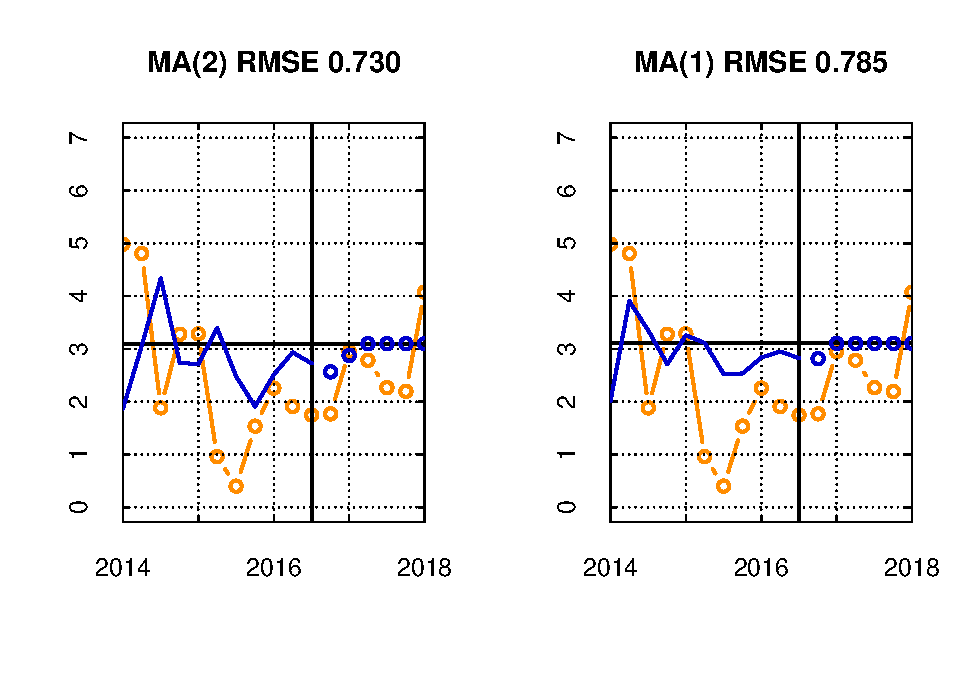
\includegraphics{_main_files/figure-latex/unnamed-chunk-65-2.pdf}

\hypertarget{exercises-1}{%
\section{Exercises}\label{exercises-1}}

\textbf{Exercise 1 (Best forecast under the square loss)}

Show that the best forecast under the square loss
\[
L(y_{t+h}, \ \hat{y}_{t+h|t}) = (y_{t+h}-\hat{y}_{t+h|t})^2
\]

for some forecast horizon \(h \in \mathbb{N}\) is
\[
\hat{y}_{t+h|t} = \mathbb{E} [y_{t+h} \ | \ y_t, \dots, y_1]
\]

\textbf{Exercise 2 (Best forecast under the absolute loss)}

Show that the best forecast under the absolute loss
\[
L(y_{t+h}, \ \hat{y}_{t+h|t}) = |y_{t+h}-\hat{y}_{t+h|t}|
\]

for some forecast horizon \(h \in \mathbb{N}\) is
\[
\hat{y}_{t+h|t} = \text{median}(y_{t+h}  \ | \ y_t, \dots, y_1)
\]

\textbf{Exercise 3 (Invertibility of MA(1))}

Consider the MA(1) process

\[
y_t = \theta \varepsilon_{t-1} + \varepsilon_t.
\]

Show that:

\begin{itemize}
\tightlist
\item
  if \(|\theta|<1\), then the process is invertible in the past observed values:
\end{itemize}

\[
 \varepsilon_t = \sum_{j=0}^{\infty} (-\theta)^j y_{t-j}
 \]

\begin{itemize}
\tightlist
\item
  if \(|\theta|>1\), then the process is invertible in the future observed values:
\end{itemize}

\[
 \varepsilon_t = \frac{1}{\theta} \sum_{j=0}^{\infty} \left(-\frac{1}{\theta}\right)^j y_{t+j+1}
 \]

\hypertarget{session06}{%
\chapter{Volatility modeling}\label{session06}}

\hypertarget{garch11-estimation}{%
\section{GARCH(1,1) estimation}\label{garch11-estimation}}

In this session, we implement the maximum likelihood estimation of the GARCH(1,1) model. We consider a Gaussian GARCH(1,1)

\[
\begin{aligned}
r_t &= \sigma^2_t z_t \\[1ex]
\sigma^2_t &= \omega + \alpha r_{t-1}^2 + \beta \sigma^2_{t-1}
\end{aligned}
\]

where \(z_t \sim \mathcal{N}(0, 1)\). The log-likelihood is (Exercise 3):

\[
\ell(\theta; r_1, \dots, r_T) = -\frac{T-1}{2}\log(2\pi) - \frac{1}{2}\sum_{t=2}^T\log\hat\sigma_t -\frac{1}{2} \sum_{t=2}^T \frac{r_t^2}{\hat\sigma^2_t}
\]

The values of the latent volatility \(\{\sigma_2^2, \sigma_3^2, \dots, \sigma_T^2\}\) can be estimated using the following filtering procedure for each given value \(\theta = (\omega, \alpha, \beta)\):

\begin{itemize}
\tightlist
\item
  set \(\hat\sigma^2_t = \hat{\text{Var}}(r_t)\)
\item
  for \(t = 2, \dots, T\) set \(\hat\sigma^2_t = \omega + \alpha r_{t-1}^2 + \beta \hat\sigma^2_{t-1}\)
\end{itemize}

We simulate the data according to the GARCH(1,1) process and compare the MLE with the true parameters.

\begin{Shaded}
\begin{Highlighting}[]
\DocumentationTok{\#\# Simulate data}
\NormalTok{t\_max }\OtherTok{\textless{}{-}} \DecValTok{1000}
\NormalTok{w }\OtherTok{\textless{}{-}} \FloatTok{0.01}
\NormalTok{alpha }\OtherTok{\textless{}{-}} \FloatTok{0.05}
\NormalTok{beta }\OtherTok{\textless{}{-}} \FloatTok{0.949}

\NormalTok{z }\OtherTok{\textless{}{-}} \FunctionTok{rnorm}\NormalTok{(t\_max)}
\NormalTok{sigma }\OtherTok{\textless{}{-}} \FunctionTok{c}\NormalTok{(}\DecValTok{1}\NormalTok{, }\FunctionTok{rep}\NormalTok{(}\ConstantTok{NA}\NormalTok{, t\_max))}
\NormalTok{r     }\OtherTok{\textless{}{-}} \FunctionTok{c}\NormalTok{(sigma[}\DecValTok{1}\NormalTok{]}\SpecialCharTok{*}\NormalTok{z[}\DecValTok{1}\NormalTok{], }\FunctionTok{rep}\NormalTok{(}\ConstantTok{NA}\NormalTok{, t\_max))}
\ControlFlowTok{for}\NormalTok{ (t }\ControlFlowTok{in} \DecValTok{2}\SpecialCharTok{:}\NormalTok{(t\_max}\SpecialCharTok{+}\DecValTok{1}\NormalTok{)) \{}
\NormalTok{  sigma[t] }\OtherTok{\textless{}{-}}\NormalTok{ w }\SpecialCharTok{+}\NormalTok{ alpha}\SpecialCharTok{*}\NormalTok{r[t}\DecValTok{{-}1}\NormalTok{] }\SpecialCharTok{+}\NormalTok{ beta}\SpecialCharTok{*}\NormalTok{sigma[t}\DecValTok{{-}1}\NormalTok{]}
\NormalTok{  r[t]     }\OtherTok{\textless{}{-}}\NormalTok{ sigma[t]}\SpecialCharTok{*}\NormalTok{z[t]}
\NormalTok{\}}
\NormalTok{r }\OtherTok{\textless{}{-}}\NormalTok{ r[}\DecValTok{100}\SpecialCharTok{:}\DecValTok{1000}\NormalTok{]}
\end{Highlighting}
\end{Shaded}

\begin{Shaded}
\begin{Highlighting}[]
\FunctionTok{plot.ts}\NormalTok{(r)}
\end{Highlighting}
\end{Shaded}

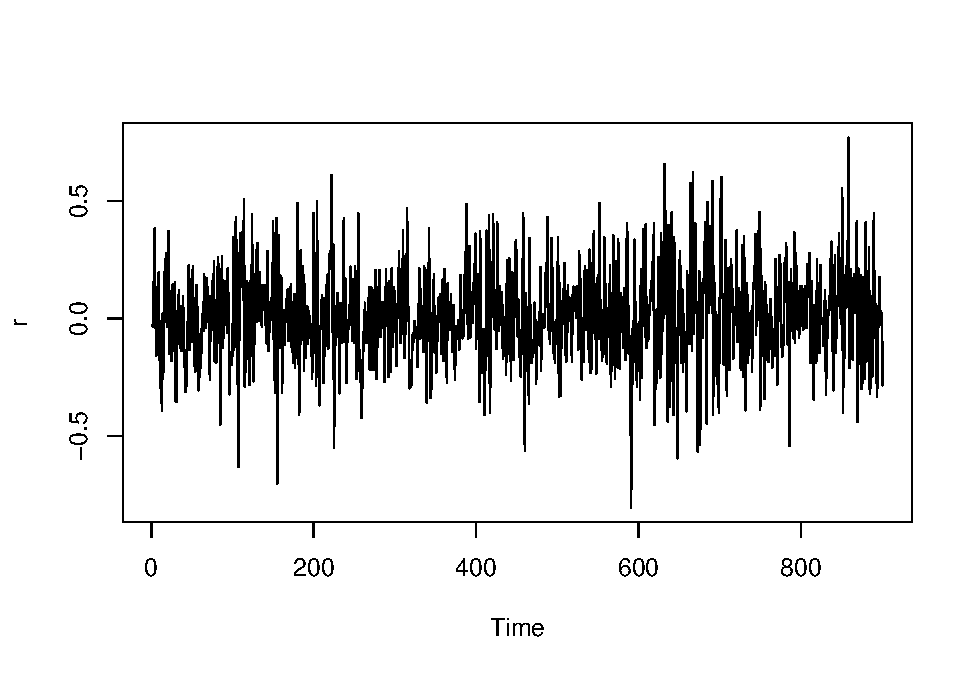
\includegraphics{_main_files/figure-latex/unnamed-chunk-67-1.pdf}

\begin{Shaded}
\begin{Highlighting}[]
\FunctionTok{plot.ts}\NormalTok{(r}\SpecialCharTok{\^{}}\DecValTok{2}\NormalTok{)}
\end{Highlighting}
\end{Shaded}

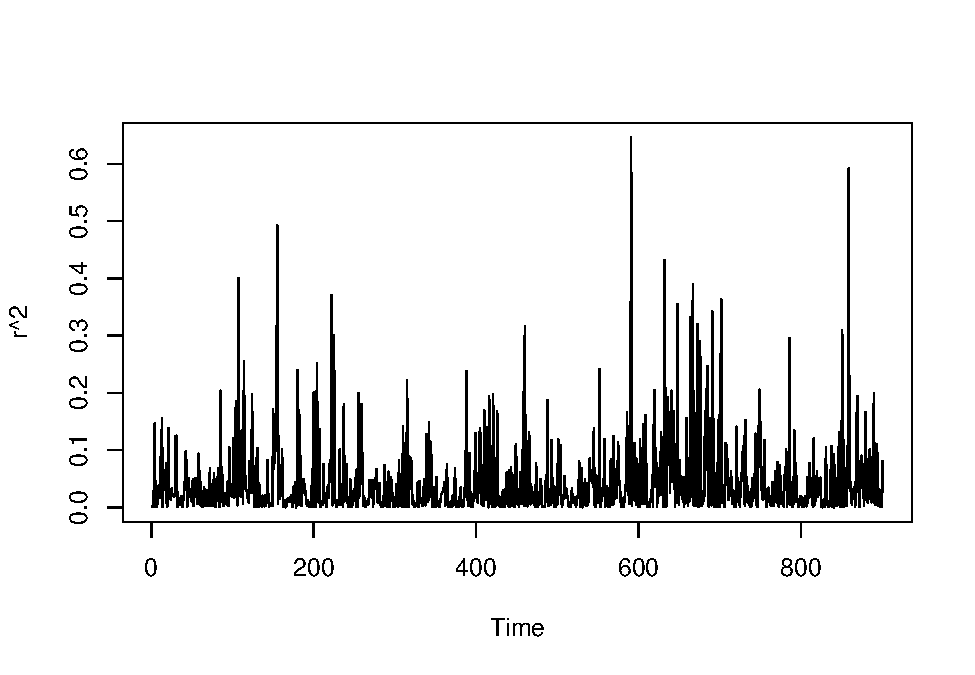
\includegraphics{_main_files/figure-latex/unnamed-chunk-67-2.pdf}

Estimation

\begin{Shaded}
\begin{Highlighting}[]
\DocumentationTok{\#\# filter }
\NormalTok{garch11\_filter }\OtherTok{\textless{}{-}} \ControlFlowTok{function}\NormalTok{(data, params)\{}
  \CommentTok{\# initializations}
\NormalTok{  omega }\OtherTok{\textless{}{-}}\NormalTok{ params[}\DecValTok{1}\NormalTok{]; }
\NormalTok{  alpha }\OtherTok{\textless{}{-}}\NormalTok{ params[}\DecValTok{2}\NormalTok{]; }
\NormalTok{  beta }\OtherTok{\textless{}{-}}\NormalTok{ params[}\DecValTok{3}\NormalTok{];}
\NormalTok{  T }\OtherTok{\textless{}{-}} \FunctionTok{length}\NormalTok{(data);}
\NormalTok{  sig2 }\OtherTok{\textless{}{-}} \FunctionTok{numeric}\NormalTok{(T); }
\NormalTok{  z }\OtherTok{\textless{}{-}} \FunctionTok{numeric}\NormalTok{(T); }
\NormalTok{  loglik }\OtherTok{\textless{}{-}} \DecValTok{0}
\NormalTok{  sig2[}\DecValTok{1}\NormalTok{] }\OtherTok{\textless{}{-}} \FunctionTok{var}\NormalTok{(data); z[}\DecValTok{1}\NormalTok{] }\OtherTok{\textless{}{-}}\NormalTok{ data[}\DecValTok{1}\NormalTok{]}\SpecialCharTok{/}\FunctionTok{sqrt}\NormalTok{(sig2[}\DecValTok{1}\NormalTok{])}
  \CommentTok{\# for loop calculating one{-}step{-}ahead}
  \ControlFlowTok{for}\NormalTok{ (t }\ControlFlowTok{in} \DecValTok{2}\SpecialCharTok{:}\NormalTok{T)\{}
\NormalTok{    sig }\OtherTok{\textless{}{-}}\NormalTok{ omega }\SpecialCharTok{+}\NormalTok{ alpha }\SpecialCharTok{*}\NormalTok{ data[t}\DecValTok{{-}1}\NormalTok{]}\SpecialCharTok{\^{}}\DecValTok{2} \SpecialCharTok{+}\NormalTok{ beta }\SpecialCharTok{*}\NormalTok{ sig2[t}\DecValTok{{-}1}\NormalTok{]}
\NormalTok{    sig2[t] }\OtherTok{\textless{}{-}}\NormalTok{ sig; z[t] }\OtherTok{\textless{}{-}}\NormalTok{ data[t]}\SpecialCharTok{/}\FunctionTok{sqrt}\NormalTok{(sig)}
\NormalTok{  \}}
  \CommentTok{\# loglik}
\NormalTok{  loglik }\OtherTok{\textless{}{-}} \SpecialCharTok{{-}}\NormalTok{T}\SpecialCharTok{/}\DecValTok{2}\SpecialCharTok{*}\FunctionTok{log}\NormalTok{(}\DecValTok{2}\SpecialCharTok{*}\NormalTok{pi) }\SpecialCharTok{{-}} \FunctionTok{sum}\NormalTok{(}\FunctionTok{log}\NormalTok{(sig2))}\SpecialCharTok{/}\DecValTok{2} \SpecialCharTok{{-}} \FunctionTok{sum}\NormalTok{(data}\SpecialCharTok{\^{}}\DecValTok{2}\SpecialCharTok{/}\NormalTok{sig2)}\SpecialCharTok{/}\DecValTok{2}
  \FunctionTok{return}\NormalTok{(}\FunctionTok{list}\NormalTok{(}\AttributeTok{sig2 =}\NormalTok{ sig2, }\AttributeTok{z =}\NormalTok{ z, }\AttributeTok{loglik =}\NormalTok{ loglik))}
\NormalTok{\}}
\end{Highlighting}
\end{Shaded}

\begin{Shaded}
\begin{Highlighting}[]
\DocumentationTok{\#\# likelihood}
\NormalTok{garch11\_objective }\OtherTok{\textless{}{-}} \ControlFlowTok{function}\NormalTok{(data, params) \{}
  
  \CommentTok{\#initializations}
\NormalTok{  omega }\OtherTok{\textless{}{-}}\NormalTok{ params[}\DecValTok{1}\NormalTok{]; alpha }\OtherTok{\textless{}{-}}\NormalTok{ params[}\DecValTok{2}\NormalTok{]; beta }\OtherTok{\textless{}{-}}\NormalTok{ params[}\DecValTok{3}\NormalTok{]}
\NormalTok{  T }\OtherTok{\textless{}{-}} \FunctionTok{length}\NormalTok{(data)}
\NormalTok{  sig2 }\OtherTok{\textless{}{-}} \FunctionTok{garch11\_filter}\NormalTok{(data, params)}\SpecialCharTok{$}\NormalTok{sig2}
  
  \CommentTok{\# if{-}else statement calculating negative loglik}
  \ControlFlowTok{if}\NormalTok{ (}\FunctionTok{all}\NormalTok{(}\FunctionTok{is.finite}\NormalTok{(params)) }\SpecialCharTok{\&}\NormalTok{ omega }\SpecialCharTok{\textgreater{}} \DecValTok{0} \SpecialCharTok{\&}\NormalTok{ alpha }\SpecialCharTok{\textgreater{}} \DecValTok{0} \SpecialCharTok{\&}\NormalTok{ beta }\SpecialCharTok{\textgreater{}} \DecValTok{0} \SpecialCharTok{\&}\NormalTok{ alpha }\SpecialCharTok{+}\NormalTok{ beta }\SpecialCharTok{\textless{}} \DecValTok{1}\NormalTok{) \{}
\NormalTok{    neg\_loglik }\OtherTok{\textless{}{-}} \SpecialCharTok{{-}}\NormalTok{(}\SpecialCharTok{{-}}\NormalTok{T}\SpecialCharTok{/}\DecValTok{2}\SpecialCharTok{*}\FunctionTok{log}\NormalTok{(}\DecValTok{2}\SpecialCharTok{*}\NormalTok{pi) }\SpecialCharTok{{-}} \FunctionTok{sum}\NormalTok{(}\FunctionTok{log}\NormalTok{(sig2))}\SpecialCharTok{/}\DecValTok{2} \SpecialCharTok{{-}} \FunctionTok{sum}\NormalTok{(data}\SpecialCharTok{\^{}}\DecValTok{2}\SpecialCharTok{/}\NormalTok{sig2)}\SpecialCharTok{/}\DecValTok{2}\NormalTok{)}
\NormalTok{  \} }\ControlFlowTok{else}\NormalTok{ \{}
\NormalTok{    neg\_loglik }\OtherTok{\textless{}{-}} \ConstantTok{Inf}
\NormalTok{  \}}
  \FunctionTok{return}\NormalTok{(neg\_loglik)}
\NormalTok{\}}
\end{Highlighting}
\end{Shaded}

\begin{Shaded}
\begin{Highlighting}[]
\DocumentationTok{\#\# MLE}
\NormalTok{garch11\_mle }\OtherTok{\textless{}{-}} \ControlFlowTok{function}\NormalTok{(data, params) \{}
  \CommentTok{\# nlminb function optimizing parameters }
\NormalTok{  fit }\OtherTok{\textless{}{-}} \FunctionTok{nlminb}\NormalTok{(}\AttributeTok{start =}\NormalTok{ params, }\AttributeTok{objective =}\NormalTok{ garch11\_objective, }
                \AttributeTok{data =}\NormalTok{ data, }\AttributeTok{lower =} \FloatTok{0.0001}\NormalTok{, }\AttributeTok{upper =} \DecValTok{1}\NormalTok{)}
  \FunctionTok{return}\NormalTok{(}\AttributeTok{param\_mle =}\NormalTok{ fit}\SpecialCharTok{$}\NormalTok{par)}
\NormalTok{\}}
\end{Highlighting}
\end{Shaded}

\begin{Shaded}
\begin{Highlighting}[]
\NormalTok{mle }\OtherTok{\textless{}{-}} \FunctionTok{garch11\_mle}\NormalTok{(r, }\FunctionTok{c}\NormalTok{(}\DecValTok{0}\NormalTok{, }\FloatTok{0.1}\NormalTok{, }\FloatTok{0.1}\NormalTok{))}
\end{Highlighting}
\end{Shaded}

\begin{Shaded}
\begin{Highlighting}[]
\FunctionTok{cbind}\NormalTok{(mle, }\FunctionTok{c}\NormalTok{(w, alpha, beta))}
\end{Highlighting}
\end{Shaded}

\begin{verbatim}
##              mle      
## [1,] 0.001443815 0.010
## [2,] 0.036959629 0.050
## [3,] 0.930826309 0.949
\end{verbatim}

\hypertarget{exercises-2}{%
\section{Exercises}\label{exercises-2}}

\textbf{Exercise 1 (ARCH(\(\infty\)) representation of GARCH(1,1))}

Show that the GARCH(1,1)

\[
\begin{aligned}
r_t &= \sigma^2_t z_t \\[1ex]
\sigma^2_t &= \omega + \alpha r_{t-1}^2 + \beta \sigma^2_{t-1}
\end{aligned}
\]
with \(\mathbb{E}[z_t] = 0\), \(\mathbb{E}[z^2_t] = 1\) can be rewritten as an ARCH(\(\infty\)) with

\[
\sigma^2_t = \frac{\omega}{1-\beta} + \alpha \sum_{j=0}^\infty \beta^j \ r^2_{t-j-1}
\]

under the assumption that \(|\beta| < 1\).

\textbf{Exercise 2 (Autocovariance of the GARCH(1,1))}

Consider the GARCH(1,1)

\[
\begin{aligned}
r_t &= \sigma^2_t z_t \\[1ex]
\sigma^2_t &= \omega + \alpha r_{t-1}^2 + \beta \sigma^2_{t-1}
\end{aligned}
\]

with \(\mathbb{E}[z_t] = 0\), \(\mathbb{E}[z^2_t] = 1\).

Show that:

\[
\gamma(k) = \text{cov}(r_t, r_{t-k}) = 
\begin{cases}
\frac{\omega}{1-\alpha-\beta}  \qquad  & k = 0 \\
0 & k \neq 0
\end{cases}
\]

\emph{{[}Difficult question{]}} Also show that

\[
\gamma_2(k) = \text{cov}(r^2_t, r^2_{t-k}) = 
\begin{cases}
\text{Var}(r^2_t - \sigma^2_t)\left[1+\frac{\alpha+2\beta}{1-(\alpha+\beta)^2}\right] \qquad  & k = 0 \\[1em]
\text{Var}(r^2_t - \sigma^2_t)\left[\alpha+2\beta+\frac{(\alpha+2\beta)^2 (\alpha+\beta)}{1-(\alpha+\beta)^2}\right] \qquad  & k = 1 \\[1em]
(\alpha+\beta)^{k-1}\gamma(1) & k \geq 2
\end{cases}
\]
where \(\text{Var}(r^2_t - \sigma^2_t) = (\mu_4 - 1)\left( \sigma_4 - \left(\frac{\omega}{1-\alpha-\beta}\right)^2 \right)\), \(\sigma^4 = \mathbb{E}[\sigma^4_t]\) (you do not need to find the explicit expression for this in terms of the parameters) and \(\mu_4 = \mathbb{E}[z_t^4]\).

\textbf{Hint:} Show that the GARCH(1,1) admits an ARMA(1,1) representation \(\sigma_t^2 = \omega + (\alpha+\beta)r^2_{t-1} + \beta(r^2_{t-1}-\sigma^2_{t-1}) + (r^2_{t}-\sigma^2_{t})\) and apply the formula for the autocovariance of the ARMA(1,1) (see Exercise 3 in Session 4).

\textbf{Exercise 3 (Log-likelihood of the GARCH(1,1))}
Consider a Gaussian GARCH(1,1)

\[
\begin{aligned}
r_t &= \sigma^2_t z_t \\[1ex]
\sigma^2_t &= \omega + \alpha r_{t-1}^2 + \beta \sigma^2_{t-1}
\end{aligned}
\]

where \(z_t \sim \mathcal{N}(0, 1)\). Show that the conditional log-likelihood of the model is

\[
\ell(\theta; r_1, \dots, r_T) = -\frac{T-1}{2}\log(2\pi) - \frac{1}{2}\sum_{t=2}^T\log\hat\sigma_t -\frac{1}{2} \sum_{t=2}^T \frac{r_t^2}{\hat\sigma^2_t}
\]

where \(\hat\sigma_t^2\) is the predicted value of the latent volatility computed using the filtering procedure described in the session.

  \bibliography{book.bib,packages.bib}

\end{document}
